\documentclass[12pt,a4paper,fleqn,oneside]{report}
%\documentclass[12pt,a4paper,fleqn,oneside]{scrartcl}
\usepackage[
    rmargin=1.2in,
    lmargin=1.2in
]{geometry}

\usepackage[utf8]{inputenc}
\usepackage{t1enc}
\def\magyarOptions{defaults=hu-min}
\usepackage[english]{babel}

%\usepackage[utf8]{inputenc}
%\usepackage[magyar]{babel}
\usepackage{tikz} 
\usepackage{longtable}
\usepackage{xurl}
\usepackage{amsmath}
\usepackage{listings}
\usepackage{t1enc}
\usepackage{tabularx}
\usepackage{ltxtable}
\usepackage{graphicx}
\usepackage{array,booktabs,enumitem}% http://ctan.org/pkg/{array,booktabs,enumitem}
\usepackage{pdfpages}
\usepackage{relsize} 

\usepackage{csquotes}

\usepackage{titlesec}
\setcounter{secnumdepth}{5}

\usepackage[
    backend=biber,
    sorting=none,
    doi=true
    ]{biblatex}

\addbibresource{src/references.bib}

\usepackage{color} %red, green, blue, yellow, cyan, magenta, black, white
\usepackage[framed, numbered]{matlab-prettifier}

\usepackage{subfigure}

\usepackage[hidelinks]{hyperref} % 
    \hypersetup{colorlinks, citecolor=, linkcolor=, urlcolor=blue}
    \renewcommand\UrlFont{\color{blue}\rmfamily\itshape} % I thought this should make it italic, but it does not
    \newcommand{\changeurlcolor}[1]{\hypersetup{urlcolor=#1}}

\definecolor{mygreen}{RGB}{28,172,0} % color values Red, Green, Blue
\definecolor{mylilas}{RGB}{170,55,241}

\lstset{
     literate=%
         {á}{{\'a}}1
         {í}{{\'i}}1
         {é}{{\'e}}1
         {ú}{{\'u}}1
         {ü}{{\'u}}1
         {ű}{{\'u}}1
         {ó}{{\'o}}1
         {ö}{{\'o}}1
         {ő}{{\'o}}1
         {Ö}{{\'O}}1
         {É}{{\'E}}1
}

\renewcommand{\maketitle}{
    \begin{titlepage}
        \begin{center}
            
\includegraphics[scale=0.1]{img/kitlogo.png}\\
            
\includegraphics[scale=0.5]{img/egyetem.png}\\
            \vspace{1cm}
            \huge\textbf{Smart home applications based on Thread network}\\
            \vspace{1cm}
            \Large{Author:}\\
            \LARGE\textbf{Márk Mihalik}\\
            \vspace{1cm}
            \Large{Supervisor:}\\
            \textbf{Dr. Balázs Matolcsy, Ph.D.}\\
            \vspace{1cm}
            \Large\textbf{Bachelor of Science}\\
            \Large\textbf{Thesis}\\
            \vspace{1cm}
            \Large\textbf{2021}
        \end{center}
        % \begin{tikzpicture}[remember picture,overlay]
        %     \node[anchor=south east,inner sep=10pt] at (current page.south east)
        %       {
\includegraphics[scale=0.9]{img/hit_logo.png}};
        % \end{tikzpicture}
    \end{titlepage}
}
\newenvironment{conditions}
  {\par\vspace{\abovedisplayskip}\noindent\begin{tabular}{>{$}l<{$} @{${}={}$} l}}
  {\end{tabular}\par\vspace{\belowdisplayskip}}

\usepackage[T1]{fontenc}

\lstdefinestyle{ascii-tree}{
    literate={├}{|}1 {─}{--}1 {└}{+}1,
    frame=single
  }
 \lstdefinestyle{tree}{
    literate=
    {├}{{\smash{\raisebox{-1ex}{\rule{1pt}{\baselineskip}}}\raisebox{0.5ex}{\rule{1ex}{1pt}}}}1 
    {─}{{\raisebox{0.5ex}{\rule{1.5ex}{1pt}}}}1 
    {└}{{\smash{\raisebox{0.5ex}{\rule{1pt}{\dimexpr\baselineskip-1.5ex}}}\raisebox{0.5ex}{\rule{1ex}{1pt}}}}1 
  }
  
\lstdefinestyle{device-tree}
{
    language=dts,
    tabsize=8,
    keepspaces,
    extendedchars=true,
    rulecolor=\color{black},
    basicstyle=\footnotesize,
    aboveskip=5pt,
    upquote=true,
    columns=fixed,
    showstringspaces=false,
    extendedchars=true,
    breaklines=true,
    frame=single,
    showtabs=false,
    showspaces=false,
    showstringspaces=false,
}

\lstdefinestyle{c-lang}
{
    language=c,
    tabsize=8,
    keepspaces,
    extendedchars=true,
    rulecolor=\color{black},
    basicstyle=\footnotesize,
    aboveskip=5pt,
    upquote=true,
    columns=fixed,
    showstringspaces=false,
    extendedchars=true,
    breaklines=true,
    frame=single,
    showtabs=false,
    showspaces=false,
    showstringspaces=false,
}

\lstset{aboveskip=\baselineskip,belowskip=\baselineskip,basicstyle=\ttfamily}

\usepackage{siunitx}
\sisetup{math-micro={\usefont{T1}{phv}{m}{n}\text{µ}}}


\begin{document}

\maketitle

\noindent
\thispagestyle{empty}
Alulírott Mihalik Márk, szigorló hallgató kijelentem, hogy ezt a szakdolgozatot meg nem engedett segítség nélkül, saját magam készítettem, csak a megadott forrásokat (szakirodalom, eszközök stb.) használtam fel. Minden olyan részt, melyet szó szerint, vagy azonos értelemben, de átfogalmazva más forrásból átvettem, egyértelműen, a forrás megadásával megjelöltem.
Hozzájárulok, hogy a jelen munkám alapadatait (szerző(k), cím, angol és magyar nyelvű tartalmi kivonat, készítés éve, konzulens(ek) neve) a BME VIK nyilvánosan hozzáférhető elektronikus formában, a munka teljes szövegét pedig az egyetem belső hálózatán keresztül (vagy hitelesített felhasználók számára) közzétegye. Kijelentem, hogy a benyújtott munka és annak elektronikus verziója megegyezik. Dékáni engedéllyel titkosított diplomatervek esetén a dolgozat szövege csak 3 év eltelte után válik hozzáférhetővé.
\newline
\newline
Kelt: Budapest, 2021. 12. 10.    


\clearpage

\renewcommand{\abstractname}{Kivonat}
\begin{abstract}
    \noindent
    Ez a szakdolgozat betekintést nyújt az új generációs Thread hálózatok felépí-tésébe, működtetésébe és a Thread mesh hálózatokban rejlő potenciális alkalmazási lehetőség-ekre. A dolgozatban a nemrégiben megjelent Nordic nRF52840-dongle modulok és saját nyomtatott áramkörök segítségével mutatom be a Thread kommunikációt több modul és egy átjáró között. Az ilyen Thread hálózatok legnagyobb előnye a vetélytársakkal szemben a kiváló skálázhatóság, mesh topológia miatt a kiemelkedően jó területi lefedettség és a megfelelően gyors adatátvitel. A Thread hálózatok egyik kiemelkedő alkalmazási területe az okosotthon(ok). Ezen felhasználási területen sokféle Thread hálózat kompatibilis eszközt kapcsolunk egy nagy egységes mesh hálózatba, és a  Thread hálózati végpontokon keletkezett szenzor/beavatkozó modul adatokat egy egységes adatbázisban tárolhatjuk, amely hozzásegít az okosotthonok szabályozási és monitoring rendszerének hatékony kialakításához. Dolgozatomban felépítek egy Thread alapú okosotthon platformot (hardver és szoftver szempontból is), amelyben egy központi egységet (Border Router) és több szenzorral ellátott végpontot (Endpoint) használok fel. Az adatok megjelenítéséhez egy grafikus felhasználói interfészt is készítettem, amely segítségével az egyes szenzoradatok megjeleníthetők, illetve az eszközök fel és lecsatlakoztathatók.
\end{abstract}
\clearpage

\renewcommand{\abstractname}{Abstract}
\begin{abstract}
    \noindent
    This bachelor thesis provides insight into the design, operation and potential applications of the new generation of Thread networks. In this thesis, I demonstrate Thread communication between multiple modules and a gateway using the recently released Nordic nRF52840 Dongle modules and my own printed circuit boards. The main advantage of such Thread networks over their competitors is the excellent scalability, mesh topology due to the outstandingly good area coverage and the sufficiently fast data transfer. One of the prominent applications of Thread networks is the smart home(s). In this application area, a large variety of Thread network compatible devices are connected to a large unified mesh network and the sensor/intervention module data generated at the Thread network endpoints can be stored in a unified database, which contributes to the efficient design of control and monitoring systems for smart homes. In my thesis, I build a Thread-based smart-home platform (both from hardware and software point of view) using a central unit (Border Router) and several sensor endpoints (Endpoint). I have also created a graphical user interface to display the data, and to connect and disconnect devices.
\end{abstract}
\clearpage


\chapter{Research}
\section{Thread}


\subsection{Introduction}
Nowadays, the term "Smart Home" is more and more often used in the media or on the internet. According to a survey by \href{https://www.statista.com/outlook/dmo/smart-home/worldwide#smart-homes}{statista.com}\cite{Statista}, the share of the global market for smart homes will reach US\$100 million by the end of 2021 and double that number by 2025. The aim of smart homes is to enable the owner or occupant of the home to easily control the devices in their home via a smartphone or over the internet. Such devices could include smart thermostats, light switches and power sockets. The examples listed above are just a small selection of the wide range of these devices, as there are countless other consumer electronics, security or control electronics (such as irrigation systems) on the market. On the other hand, it is also very important to minimise energy consumption, as environmental protection is becoming increasingly important in society and it is not always possible to supply a thermostat with continuous mains voltage. The \href{https://www.threadgroup.org/}{Thread}\cite{threadgroupurl} provides a solution to this market and these problems.
It is also safe, as the possibility of connection is limited to a given device (this process will be discussed in detail in a later section) and communication is only between devices on the same network. The network topology is considered reliable as several devices are connected to several devices (mesh networking), so that if one device fails, the entire subnetwork does not collapse. This is also due to the fact that devices dynamically choose their role in the network. Low-power Thread devices can run for years on a single lithium coin-cell battery. Last but not least, thousands of devices can be connected to a Thread network, providing a potential solution for connecting devices in smart offices.

\subsection{Thread comparison with other protocols}
First of all, this thesis discusses the differences between well known mesh protocols, like ZigBee and Bluetooth Mesh and compares the differences between them. Finally the Wi-Fi is also compared, which is the most widely used wireless radio protocol in the whole world.\cite{threadcompare}\cite{threadcomapare2}

\subsubsection{Thread vs. ZigBee}
ZigBee is the closest data link protocol to Thread. It's physical layer and the \textit{Medium Access Control} (short \textbf{MAC}) layer in the data link layer are defined by the same standard as IEEE 802.15.4. The modulation type is \textit{Carrier sense multiple access/collision avoidance} (short \textbf{CSMA/CA}), which ensures good, secure data transmission on unused channels. Thus, both communications have a data rate of 250\,\si{\kilo bit/s}, making the use of this technology for smart home solutions a highly reliable and low latency solution. This standard defines three different frequencies as carrier frequencies, but the most relevant one used in my bachelor's thesis is 2.4\,\si{\giga\hertz}, because both protocols are based on it. This range falls in the ISM (Industrial, Scientific, Medical)  band in all countries and therefore does not require a licence. Thread protocol was specified in 2016 and has significant innovations compared to ZigBee which has been in development since 2003. Thread is a self-healing mesh network based on IPv6 (as opposed to Zigbee, which is based on IPv4) and is designed for low-power IoT device communication. Unlike IPv4 addressing, which uses a 32-bit number (4.3 billion distinct addresses can be reserved), IPv6 uses 128-bit numbers for addressing, giving $3.4 \cdot 10^{38}$ distinct addresses for devices and dedicated IP addresses. This method allows each device to have an unique address, thus facilitating the role of the router in the Internet world. On the other hand the devices determine their own roles in the Thread network dynamically. Both protocols (Thread and ZigBee) fully map the network and determine the endpoint for each packet. For both, a single coin-cell battery is sufficient to power the device up to few years.

\subsubsection{Thread vs. Bluetooth Mesh}
Bluetooth Mesh offers a solution for the automation of industrial buildings and smart homes. Unlike the former, it is based on the IEEE 802.15.1 standard and within it \textit{Bluetooth Low Energy} (short \textbf{BLE}). The advantage of this protocol is that all layers involved in the network model are controlled by the Bluetooth Special Interest Group. BLE also uses the 2.4\,\si{\giga\hertz} carrier frequency with GFSK (Gaussian frequency-shift keyring) modulation. Unlike Thread, Bluetooth Mesh uses flooding to send information to endpoints, which has the disadvantage that it can hold up packets, increasing the latency of a packet. One of its advantages over Thread is that it can send up to four times more data per second. Like Thread and ZigBee, devices with this BLE protocol also can be powered with a coin-cell battery.

\subsubsection{Thread vs. Wi-Fi}
Wi-Fi technology has been around since 1997 and is the most widely used protocol for wireless data transmission. The currently most widely used Wi-Fi 5 (802.11ac) can reach 3.5\,\si{\giga bit/s}, that is 14000 times faster than Thread. However, this speed comes at a cost, as the transceiver module can draw much more power, so powering it from a single coin-cell battery is an impossible task and it requires constant power source (e.g. from power line). Basically the Wi-Fi system has a star point network topology, where a router is the central element of the network, where the devices can be connected, but mesh networking is also supported in the latest Wi-Fi 6. It is commonly referred to as the best speed vs. energy efficient communication method, but it is unsuitable for small and extra low power devices. 


\subsection{Latency comparison between Thread, ZigBee and Bluetooth Mesh}
Silicon Labs conducted a larger scale measurement with their own devices to compare the difference between the latencies of Thread, ZigBee, Bluetooth Mesh. Furthermore, they also made a measurement of the distribution of latencies. These three solutions target the same low-power IoT device market. This measurement was carried out in a large office building. I present two measurement cases in this thesis section.

\subsubsection{First measurement}
\begin{figure}[!htb]
    \centering
    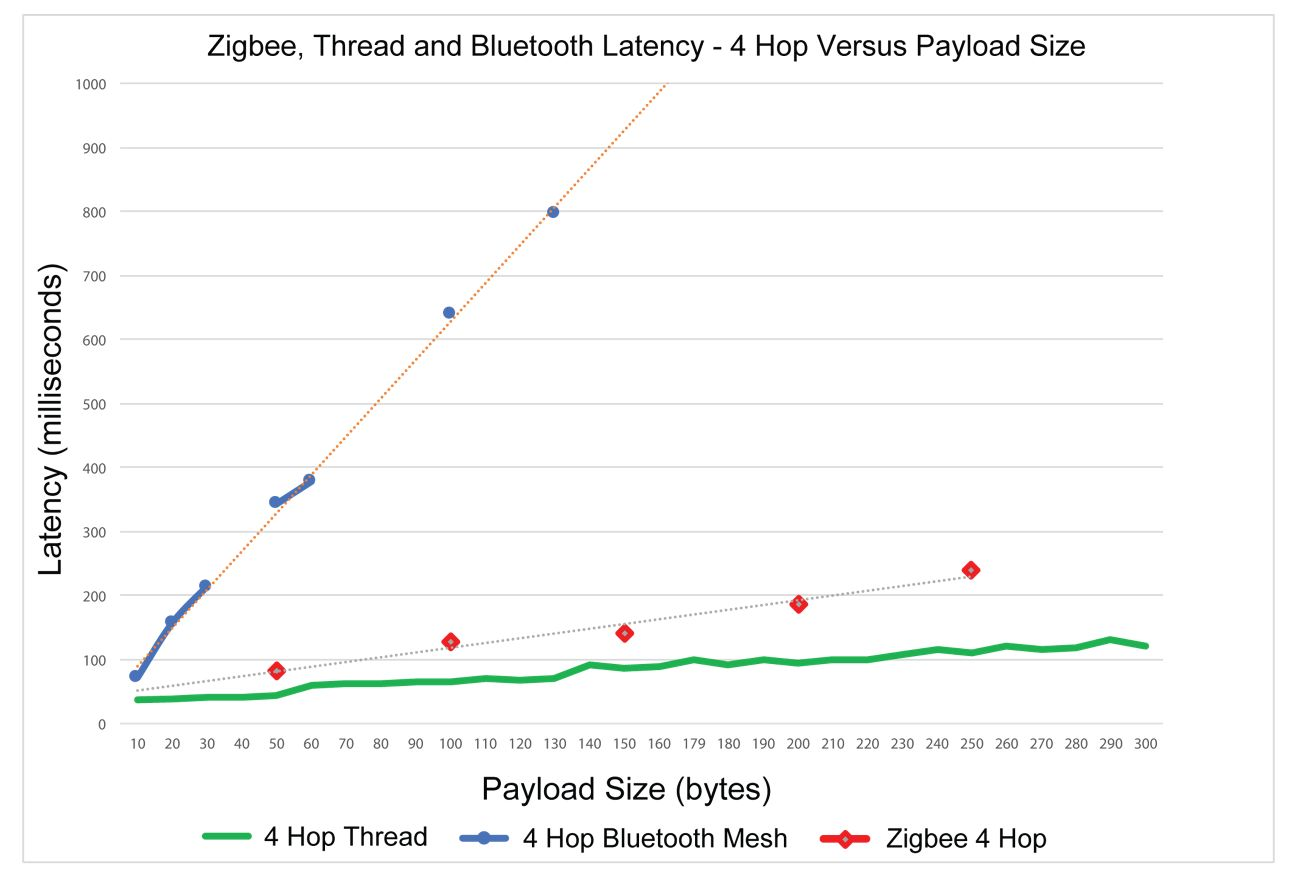
\includegraphics[width=\textwidth]{img/mesh-latency-over-four-hops.png}
    \caption{Mesh network latency between four devices}
    \label{fig:threadoverfourhops}
    \cite{threadSilabs}
\end{figure}
\noindent
The first measurement shows how the latency depends on a given data packet size across four devices. This measurement is presented in Figure \ref{fig:threadoverfourhops}, which shows the latency for very small data (10 bytes). In all three cases there is only very little difference in latency. As the size of the data increases, the latency increases in all cases in different degrees. The measurement results show that as the data packet size increases for Bluetooth Mesh (blue dots), the latency also increases dramatically compared to Thread (green line) and ZigBee (red dots). ZigBee produces much better results than Bluetooth Mesh, but Thread has the smallest slope of the approximate line. However, this measurement only tests the latency dependence between four devices, which is not the intended use of mesh networks, as the point of a mesh network is to have many small devices, up to thousands, connected to each other.


\subsubsection{Second measurement}
\begin{figure}[!h]
    \centering
    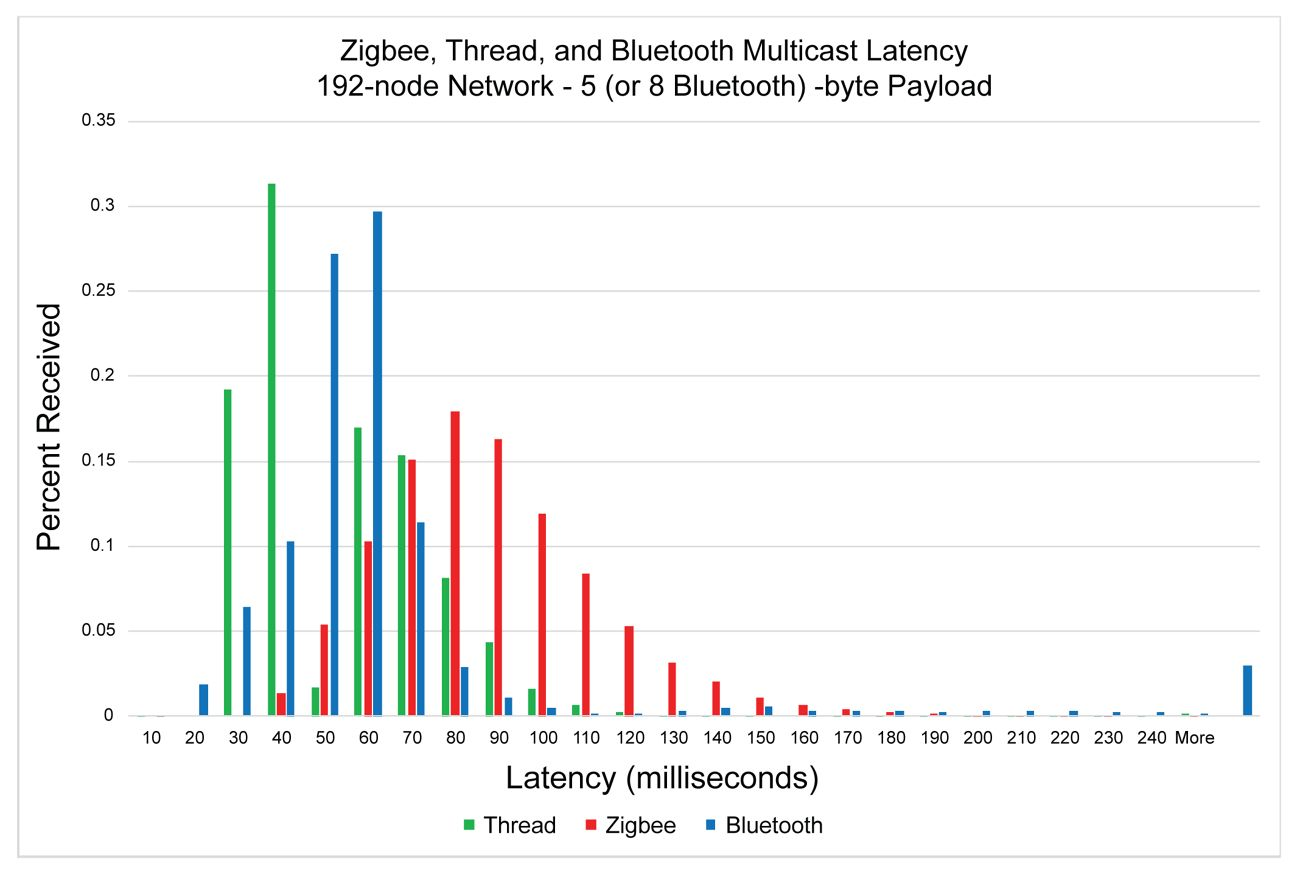
\includegraphics[width=\textwidth]{img/mesh-large-network-small-payload.png}
    \caption{Latency distribution of mesh networks for small data}
    \label{fig:threadsmallload}
    \cite{threadSilabs}
\end{figure}
\noindent
The second measurement tests a mesh network with 192 devices with small (5-8 bytes) and medium (16-25 bytes) data packets and examines the latency distribution.
\newline
For small data, the latencies are distributed as shown in Figure \ref{fig:threadsmallload}. From this, the convention can be drawn that on average, data arrived in 50\,\si{\milli s} for Thread, which performs the best of all mesh networks that were examined. The second best performing is the Bluetooth Mesh, with data arriving in 60\,\si{\milli s} most of the time. However, it is important to note that in 5\% of the measured results, the latency is more than 100\,\si{\milli s}. In the case of Thread, all data arrives in less than 120\,\si{\milli s}. ZigBee performs the worst in this measurement, with an average of 80\,\si{\milli s}, but 190\,\si{\milli s} is the longest delay.

\begin{figure}[!h]
    \centering
    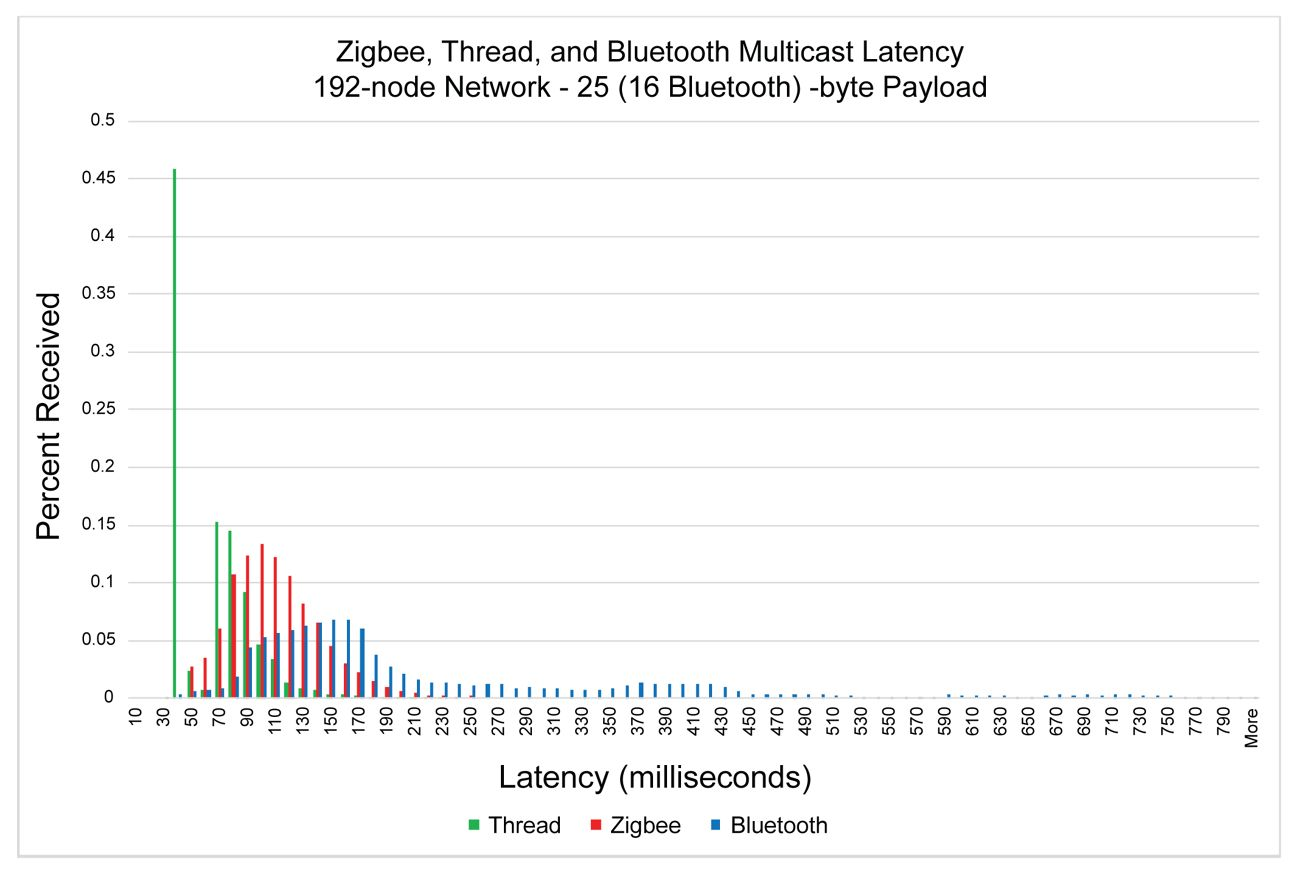
\includegraphics[width=\textwidth]{img/mesh-large-network-moderate-payload.png}
    \caption{Latency distribution of mesh networks for medium data}
    \label{fig:threadmoderateload}
    \cite{threadSilabs}
\end{figure}
\noindent
For larger data, the measurement results are shown in Figure \ref{fig:threadmoderateload}. For Thread, most data reaches the endpoint in 50\,\si{\milli s} on average. This is followed by ZigBee, where this number is 100\,\si{\milli s}. Bluetooth Mesh performed the worst, with data arriving in 150\,\si{\milli s}. It is also important to look at the extreme values. For Thread, the maximum latency is 170\,\si{\milli s}, for ZigBee it is 250\,\si{\milli s} and for Bluetooth Mesh it is up to 750\,\si{\milli s}. From an automation point of view, 750\,\si{\milli s} is not a large delay for a light or a door opener, but for a user to switch these devices using their mobile phone, this would be a very large, noticeable delay.
\newline
The final conclusion from these measurements is that, the Thread performs best in data latency. Thus, for places where data transfer rates of 250\,\si{\kilo bit/s} are sufficient, Thread is the best choice, as it can provide a stable connection with low latency and low power consumption.


\subsection{Thread network}
\begin{figure}[!htb]
    \centering
    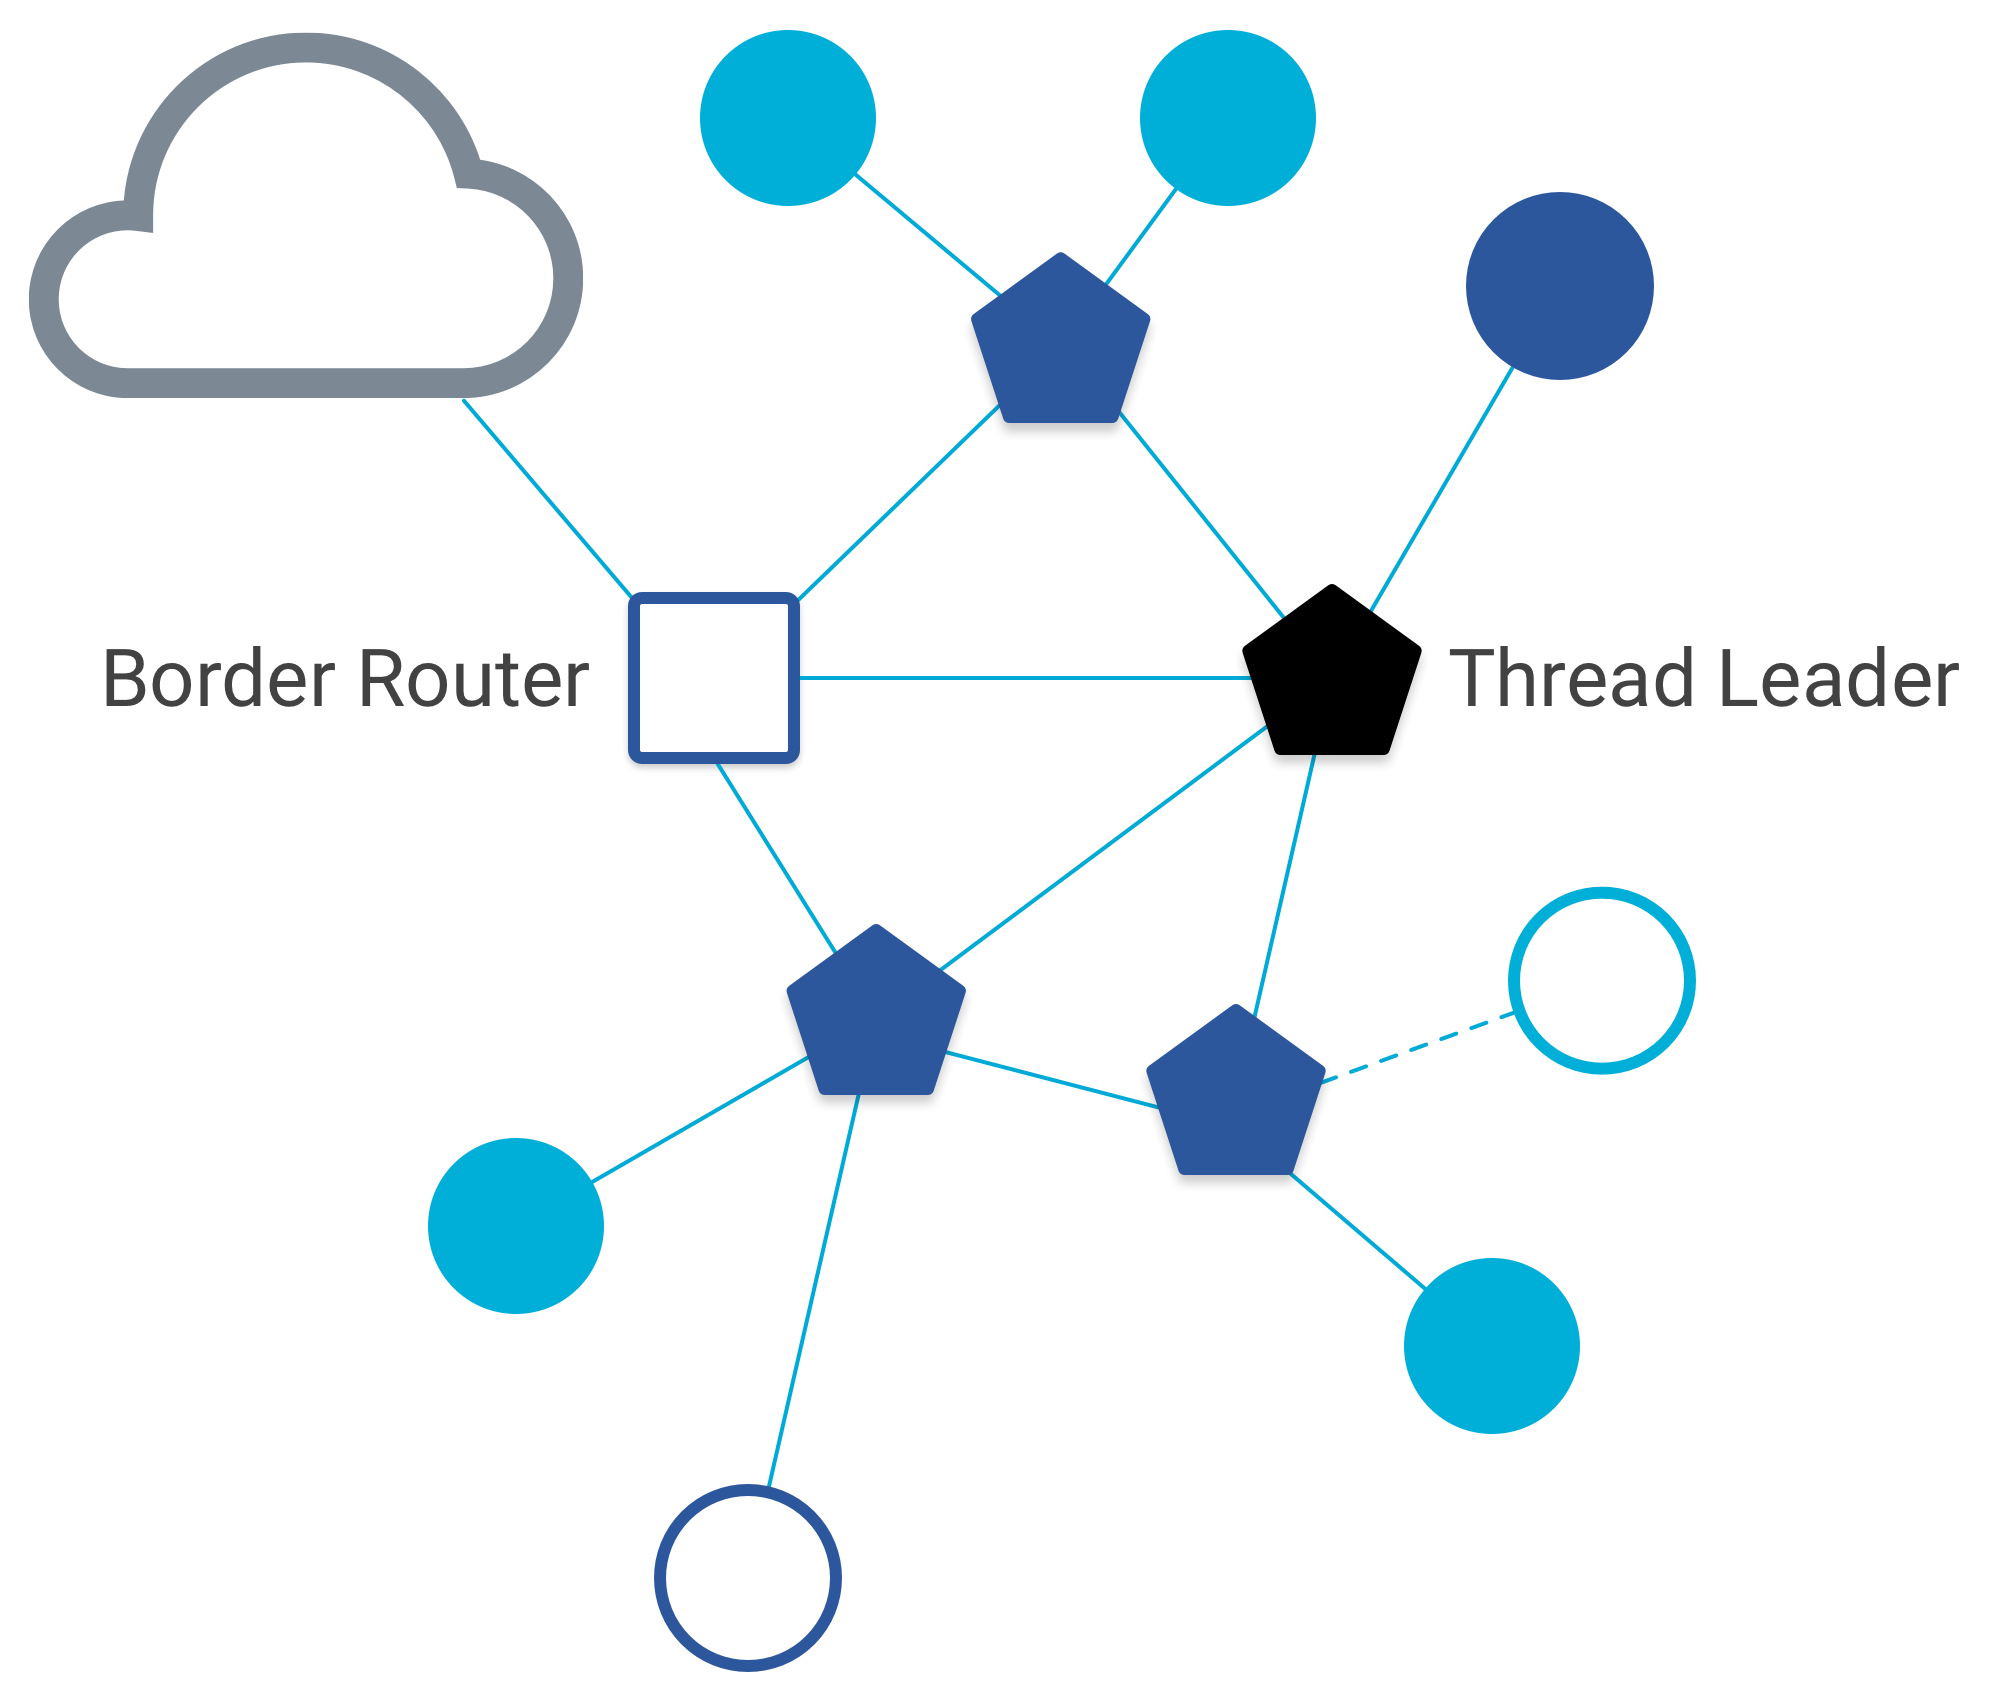
\includegraphics[scale=0.14]{img/ot-primer-leader_2x.png}
    \caption{Thread network topology}
    \label{fig:thread_network}
    \cite{thread_network}
\end{figure}
\noindent
Figure \ref{fig:thread_network} shows a typical Thread network topology. Each blue pentagon represents a Router. These devices can be connected to by so-called End Devices. It is important to note that two types of devices are defined within the Thread protocol. One is the \textit{Full Thread Device}, abbreviated \textbf{FTD} and the other is the \textit{Minimal Thread Device}, abbreviated \textbf{MTD}. The former is recommended in an environment where the continuous power supply for the device is provided (e.g. 230\,\si{\volt} power supply). Because only this kind of devices can form the backbone of the network (see pentagons). Since these devices are responsible for maintaining and managing the IP address topology and sending data within the Thread network. The RF transceiver of Thread FTD devices is always on and subscribes to the multicast address (a pre-booked IP address that can be used to reach a group of devices) of each router and must therefore handle multicast requests. This results in increased power consumption, with a current consumption of 12-15\,\si{\milli\ampere} at a supply voltage of 5\,\si{\volt}, which shows that this devices would not meet the requirement of being able to operate for years from a single coin-cell battery. This problem is solved by Thread MTD devices. As these devices can only communicate with the router or also known as the Parent device. These devices are then called Child and only need to serve requests from the Router, further reducing power consumption. This document refers to Figure \ref{fig:thread_network} in parentheses at the end of the following lists for clarity.
\noindent
FTD devices can perform three functions, which can be\cite{OpenThreadNodeType}
\begin{itemize}
    \item Router (dark blue filled pentagon) --- device that performs network functions,
    \item Router Eligible End Device - REED --- able to designate itself as a router (dark blue filled circle),
    \item Full End Device - FED --- not able to designate itself as a router (dark blue unfilled circle).
\end{itemize}
\clearpage
\noindent
Furthermore, there are three specific states of an FTD device, which are 
\begin{itemize}
    \item Thread Leader (black filled pentagon) --- router management device,
    \item Border Router (dark blue square) --- gateway/transmitter between Thread and other network,
    \item Commissioner (not shown) --- device that performs connectivity.
\end{itemize}
MTD devices can be equipped with two special conditions
\begin{itemize}
    \item Minimal End Device - MED --- in constant contact with the parent,
    \item Sleepy End Device - SED --- is usually in a sleeping state and needs to interrogate the parent upon waking.
\end{itemize}
In this section I introduced the types of devices in a Thread network, but it is important to highlight some of the more important roles.


\subsection{Detailed description of Thread network roles}
\subsubsection{Role of Router}
As I mentioned in the previous section in the case of a Router, the transceiver is always on, as these devices are always FTDs. It's main tasks are to forward packets between devices and to communicate with End Devices. It's special role can be that only these units can connect a new device to the Thread network. I'm going to discuss this process later for the Commissioner.

\subsubsection{Role of End Device/Child}
In this role there is a difference in the operation between MTD and FTD devices, but they have one thing in common. These devices are only connected to one Router and can only communicate with it. They cannot send data directly to other units.
For MTD devices, the transceiver can be optionally disabled to reduce power consumption.

\subsubsection{Role of Thread Leader}
These devices are unique to a Thread network and have the specific task of controlling Router devices and managing configuration information for the entire network. These devices (Routers) dynamically assign themselves to this task to reduce the chance of network failure. The possibility of reassigning device roles usually occurs every 130 seconds. 

\subsubsection{Role of Border Router}
These devices are able to establish a connection between a Thread network and an external network, for example they can act as a gateway. An external network can be an Ethernet network, such as the one I implemented in my bachelor's thesis. Any device can act as a Border Router, there is no restriction, but it is worth choosing an FTD device for this purpose, because it allows continuous communication with the outside world. 

\subsubsection{Role of Commissioner}
As I mentioned in the role of routers, this is an extra task that only Routers can handle. This task is nothing more than connecting new devices to the network. This commissioning is done with an identifier stored in a unique chip called eui64. If this unique identifier is recognised by the Commissioner, the device to be connected can connect to the network using the Joiner password. The Thread Group, Google's developer of OpenThread, also offers various solutions to the connectivity problem, that are as ready-made solutions for developers and users alike.

\subsection{IPv6 addressing within a Thread network}
\begin{figure}
    \centering
    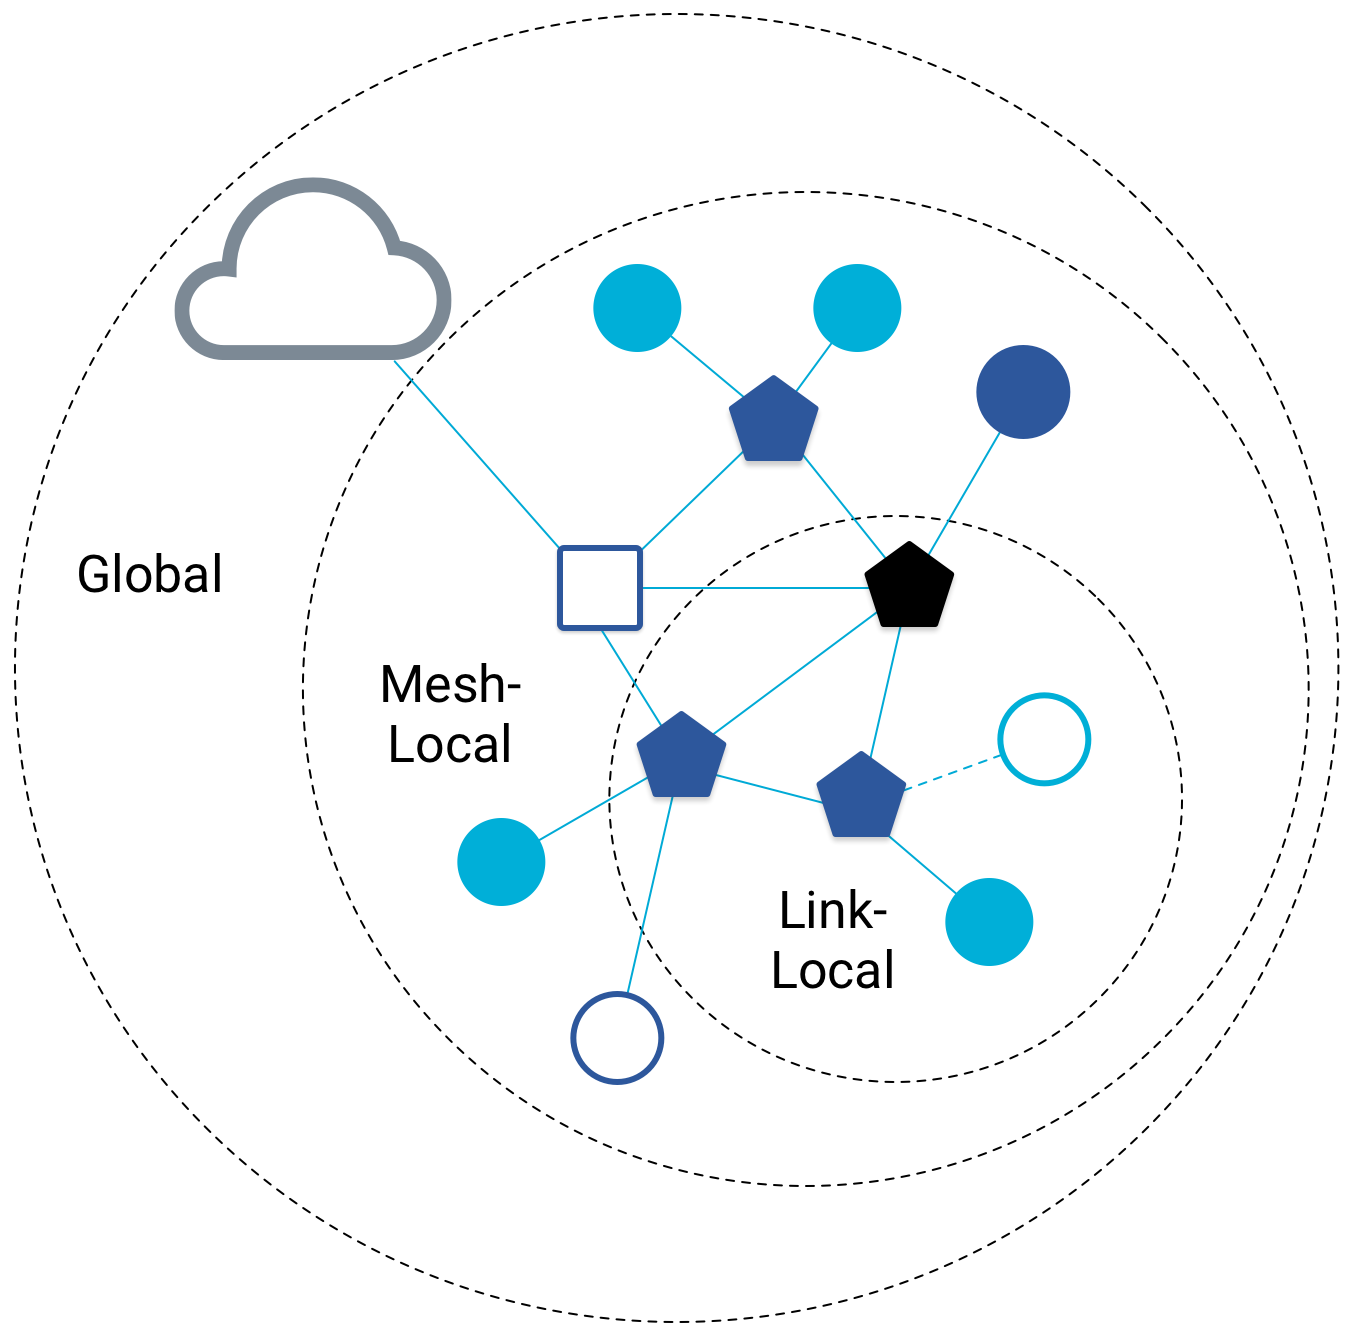
\includegraphics[scale=0.16]{img/ot-primer-scopes.png}
    \caption{Thread network allocation}
    \label{fig:thread_scope}
    \cite{thread_scope}
\end{figure}

Figure \ref{fig:thread_scope} shows that a network can be divided into three main parts.\cite{ThreadIPv6}
\begin{itemize}
    \item Link-Local - prefix: fe80::/16 --- This network contains the devices that are adjacent to each other, i.e. they are reachable by a radio transmission. Generally used to map neighbouring devices.
    \item Mesh-Local - prefix: fd00::/8 --- This network contains all devices that are connected to the given Thread network.
    \item Global - prefix: 2000::/3 --- Devices in this network are accessible from outside the Thread network.
\end{itemize}

\subsubsection{Mesh-Local address role}
These addresses have a more complex function and can be used to send data within the network. They can be divided into two groups, which are
\begin{itemize}
    \item Routing Locator,
    \item Mesh-Local EID.
\end{itemize}
The address \textit{Routing Locator}, also known as \textbf{RLOC} is used to infer the location of a device in the network and also the role of that device. With the \textit{Mesh-Local Endpoint Identifiers} (short \textbf{EID}) any device can be reached within the same Thread network. The Mesh-Local address is the most important one in my bachelor's thesis, as it is the address that allows us to reach all devices connected to the network from the Border Router device such as send and receive information. I am going to show an example of how to manage own devices and send data to them from a website later on.


\subsection{The CoAP protocol}
The \textit{Constrained Application Protocol} or \textbf{CoAP} is an information transfer server-client connection protocol specifically designed for IoT devices. It is very similar to the HTTP protocol known from the Internet, but since IoT devices are often low-powered, HTTP's implementation would consume a lot of resources and thus increase the cost of producing the devices. CoAP is a solution to this problem, taking up to 10\,\si{\kilo B} of RAM and 100\,\si{\kilo B} of code memory from the device's resources.\cite{coap_ram}
\begin{figure}
    \centering
    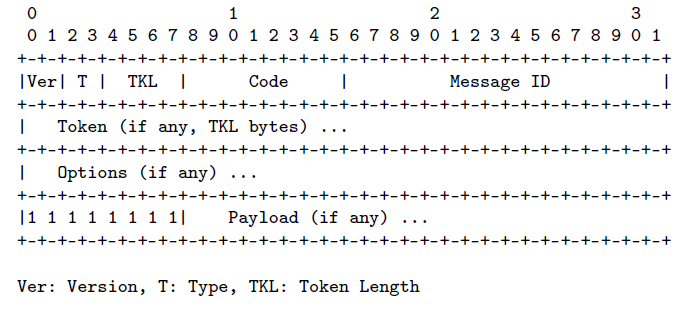
\includegraphics[width=\textwidth]{img/coapframe.png}
    \caption{Format of a CoAP message}
    \label{fig:coapmessage}
    \cite{coapcheat}
\end{figure}
Figure \ref{fig:coapmessage} shows how a CoAP message is constructed. The first two bytes represent the version number and the next two bytes contain the message type, which can take four different values.

\begin{itemize}
    \item Request type messages (Request)
        \begin{itemize}
            \item 0 - \textbf{CON}firmable --- This message type is waiting for an ACK response.
            \item 1 - \textbf{NON}-confirmable --- No response is expected from this message type.
        \end{itemize}
    \item Response type messages (Response)
        \begin{itemize}
            \item 2 - \textbf{ACK}nowledgement --- Confirming response message (see confirmable).
            \item 3 - \textbf{R}e\textbf{S}e\textbf{T} --- This message indicates that the message has been received but the processing result is unsuccessful.
        \end{itemize}
\end{itemize}
\noindent
On Figure \ref{fig:coapmessage}, the \textit{Token Length} (short \textbf{TKL}) indicates the length of the optional symbol (Token) part in four bits. Then the following one-byte code part (\textit{Code}) can be divided into two parts, a three-bit type (\textit{Class}) and a four-bit code (\textit{Code}). Suppose that the client sends a GET request to the server. The request methods are of class 0 and specifically the GET method is denoted by the value 1. If we want to denote this on paper, we separate the class and the code with a dot, so the GET request is denoted by 0.01. The \textit{Message ID} (short \textbf{MID}) is a 16-bit number used to avoid possible message duplications. The Token part is an automatic client-generated number of length defined in the TKL, which must be returned to the server without modification. The purpose of the Token is to allow the client to pair the response to the request. The settings section contains the settings related to the message, such as the address (Uri-Path) used by the intended devices to make the queries or the type of the message content, which can be either a UTF-8 encoded text or even a JSON format. In that case, when the device is needed to save memory, the application should be implemented with CBOR, which has a similar structure to JSON, but the data is encoded in binary format. So the result is more compact, smaller, but not human-readable. After that, a part of one byte and 0xFF separates the actual data from the parts we have seen so far. The detailed specification of the CoAP protocol is available at \href{https://datatracker.ietf.org/doc/html/rfc7252}{datatracker.ietf.org}\cite{datatracker}

\subsection{Summary of Thread}
In this section, I compared three different mesh networking protocol, namely Thread, ZigBee and Bluetooth Mesh and one other protocol, which can operate as a mesh network, Wi-Fi. The basis of this comparison was the power consumption, data speed and the measured latency. On the other hand, the device roles in the Thread network were presented together with the full topology and the CoAP protocol used by OpenThread.
\section{Zephyr Project}


\subsection{Introduction}
Since Thread is a protocol for low-power, energy-efficient devices and its target market is smart homes, it is important to design devices that can meet the former criterion while maintaining high computing power. Modern microcontrollers with ARM Cortex-M cores are produced by a number of manufacturers with different peripherals, sometimes with very low power consumption. There are also solutions that integrate a radio module on-chip. These manufacturers, such as Nordic, Silicon Labs or STM, produce various free SDKs to facilitate the programming of their controllers. For the protocol uses the IEEE 802.15.4 standard. Nordic Semiconductors provides a separate SDK to support Thread access. However, in many cases, learning a new SDK is a dead time for a company, not to mention that if a company is designing universal devices using only some of the capabilities offered by the devices, they will have to modify their code for each device. Zephyr offers a solution to these problems.


\subsection{Zephyr Project}
The Zephyr Project is often referred to as a real-time operating system that targets processors with microcontrollers and other architectures used in embedded systems, but its architecture is much more complex, because in reality the operating system is only a small layer of the whole. It is essentially an open source project, associated with the Linux Foundation and designed to be implemented in safety-critical systems. 
The Zephyr OS can be broken down into three main parts
\begin{itemize}
    \item Kernel --- memory management, interrupt management, timing management etc.,
    \item Operating System Services --- peripheral management, hardware module management, error handling, etc.,
    \item Application Services --- management of paired devices (e.g.: Sensors), management of Internet protocols (e.g.: CoAP).
\end{itemize}


\subsection{Zephyr RTOS properties}
The \textit{Zephyr Real-Time-Operating-System}, or \textbf{RTOS}, has the following features
\begin{itemize}
    \item multithreading,
    \item interrupt handling,
    \item memory management,
    \item inter-thread messaging (between Zephyr OS Tasks),
    \item power management,
    \item memory protection (e.g.: overflow protection).
\end{itemize}

\subsection{The purpose of the Zephyr Project}
One of its main features, besides RTOS, is that it is very easy to compile the written source code to several kinds of devices without modifying the source code, only the settings. Another important feature is that there are third-party libraries implemented in the Zephyr project, so they are easy to use (such as OpenThread).

\begin{figure}[!htb]
    \centering
    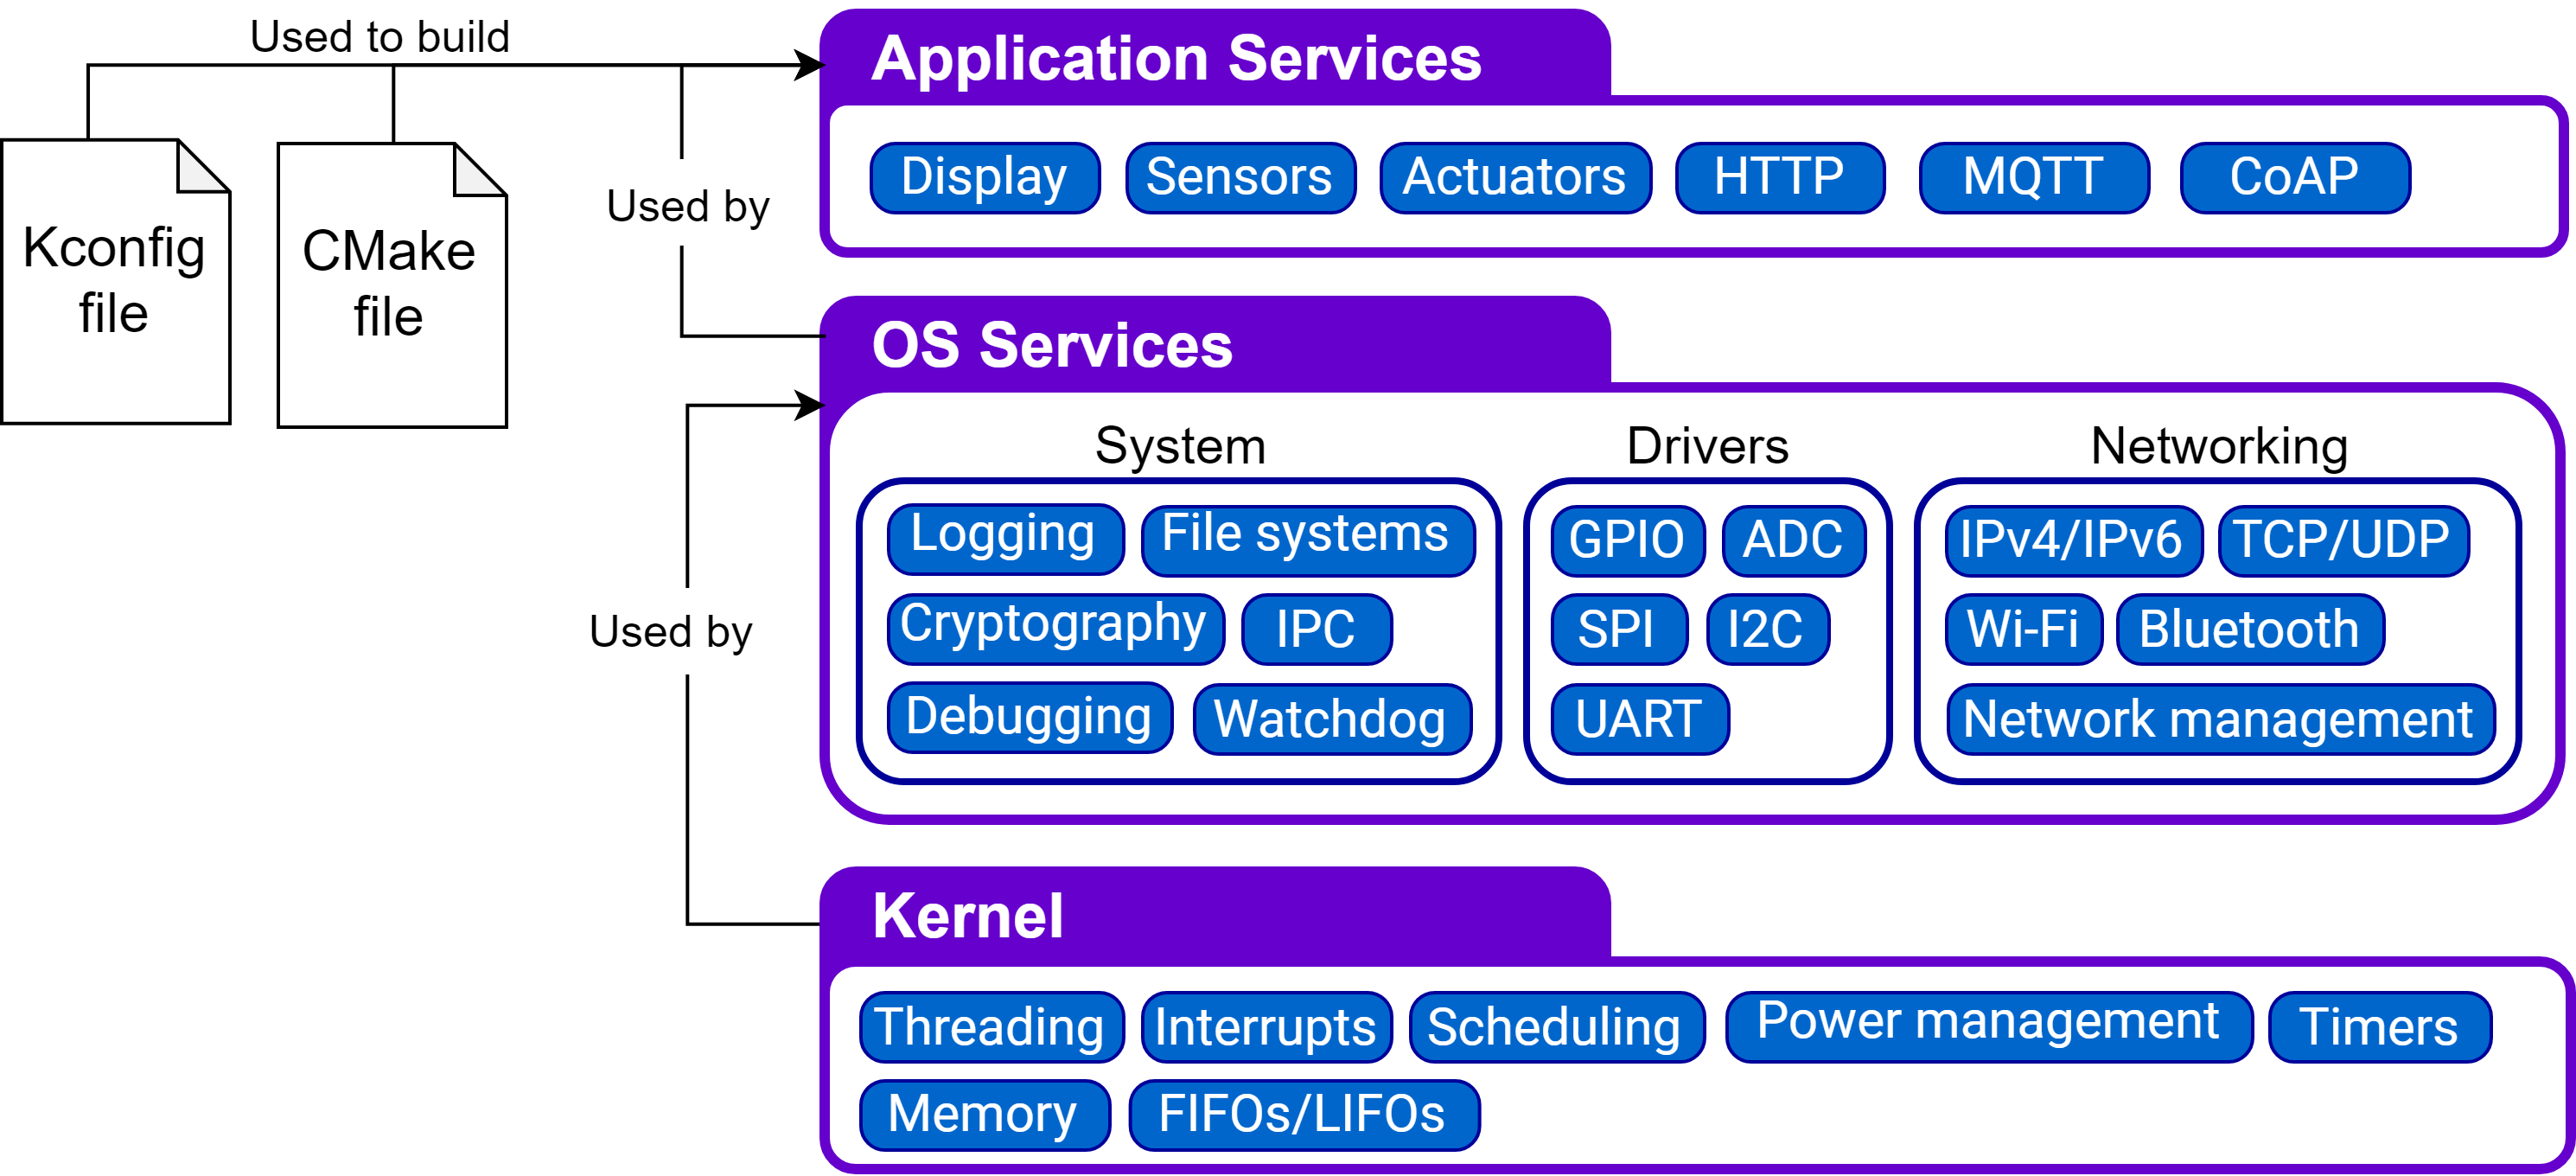
\includegraphics[scale=0.13]{img/Module_organization.png}
    \caption{Zephyr Project structure}
    \label{fig:Zephyrl}
    \cite{Zephyr}
\end{figure}


\subsection{Zephyr Project - Other programmes}

\subsubsection{DeviceTree}
It is also important to note that the Zephyr Project is cross-platform, i.e. available on Linux, MacOS and Windows operating systems. Zephyr uses \textbf{DeviceTree} to describe the hardware and for hardware portability. Essentially, in the configuration file of this program, certain functions can be named (such as LED1 or BUTTON0) or the address can be described of a particular register (such as I2C). This is advantageous because if the developer want to port a program to other hardware, only need to modify the DeviceTree description file (mostly files with .dts). For example, on an STM32F4 microcontroller, if there is a button placed, named BUTTON0 on GPIO24 and then do the same on an nRF52 for P0.31, the developer does not have to modify the code by mapping the different HAL libraries to each other, because Zephyr will do that for the developer. The hardware in this document was designed with a Nordic nRF52840 chip. Nordic Semiconductor has made two official releases of hardware with this chip, one is a development board called Development Kit (nRF52840DK) and the other is a Dongle, which can act like a module. The official use of this chip is to make a radio transceiver over an USB connection with the nRF Connect application. The dts description files for both hardware can be found pre-written in Zephyr, so by rewriting 1 line the whole source code was able to compiled from the Development Card to the Dongle, before the hardware design process.

\subsubsection{KConfig and CMake}
For software portability of the code, Zephyr uses \textbf{KConfig} to compile the used modules and drivers into the executable code at compile time. This program also helps to enable services and kernel modules when compiling the Linux kernel. The development also requires \textbf{CMake}, which adds the header and source files of the libraries to the project based on the path.

\subsubsection{Comparison of DeviceTree and KConfig}
In summary, the DeviceTree program does the hardware description, enables or disables hardware elements, enables interrupts and also sets the clock, from which it will set the microcontroller or processor at boot time. KConfig, on the other hand, will compile drivers and other libraries into Zephyr at compile time. Here is an an example of this for the better understanding. There are two applications in the same hardware environment with a controller, in which an I2C and a UART peripheral integrated. On the hardware there is an LED that is connected to a specific GPIO pin. One application the data is read from an I2C BME280 sensor and in the other case a LED is blinked. Since the same hardware must be used, the same DeviceTree descriptor structure is enough. From a software point of view, the I2C driver in the first application is needed, so KConfig should indicate this. Since the program only the I2C driver uses, KConfig will not include the other drivers at compile time, so the UART driver will not be included in the final code. In the second program, the same will happen, but the program code will not include the I2C driver.

\clearpage
\subsubsection{Example of the DeviceTree file structure}
\begin{lstlisting}
{
        compatible = "nordic,nrf-timer";
	status = "okay";
	reg = < 0x40009000 0x1000 >;
	cc-num = < 0x4 >;
	interrupts = < 0x9 0x1 >;
	prescaler = < 0x0 >;
	label = "TIMER_1";
};
\end{lstlisting}
\noindent
In this snippet of the DeviceTree file above, a timer is defined. This is an nRF timer built into a Nordic chip, which is enabled in the system (status="okay";). The address of the register block can be seen where this timer is located and how much space is reserved for this timer. The number of CC registers is 4. These are comparison registers whose function is to give an interrupt when the timer counter reaches the number stored in this registers. The interrupt is defined separately in the file what these values mean. And the penultimate line shows that this timer has no prescale. Furthermore, this timer will be referred in Zephyr as TIMER\_1. In this Nordic chip's documentation, it is able to find that the timer and actually has this register value associated with it. These .dts files own default values can be overwritten with an *.ovarlay file in the workspace directory of the program (or in some cases to the "boards" folder), where can be set the desired value by reference (for example by the status keyword, when the developer set "okay" to "disabled" and then this unit will be disabled).
\newline

\subsection{Nordic nRF52840}
The nRF52840 is a Nordic Semiconductors microcontroller, released in late 2017, designed for the 2.4\,\si{\giga\hertz} wireless market. The company provides a complete software SDK for Thread, Zigbee, Bluetooth LE (Low Energy) and Bluetooth Mesh networks. The code is executed by an ARM Cortex M4 core with a floating-point operation execution unit. It has 1\,\si{\mega B} of flash and 256\,\si{\kilo B} of RAM, which is only 30\% of the RAM and flash memory occupied by the complex OpenThread code of the Zephyr. It also has an internal DC/DC converter and an LDO so that it can be powered from its external USB power supply. Power is provided for external components through using DC/DC converter and LDO together. The maximum load current of the voltage converter's output is 25\,\si{\milli\ampere} according to the datasheet. The output voltage can be adjusted between 1.8\,\si{\volt} and 3.3\,\si{\volt} by setting two dedicated registers. It features ARM CryptoCell technology, which reduces the time needed to perform various encryptions. The IC also includes a number of communication peripherals such as USB\,2.0, QSPI, 32\,\si{\mega\hertz} SPI and several other timers and ADC modules. A full list of these functions are available on the second page of \href{https://infocenter.nordicsemi.com/pdf/nRF52840_PS_v1.1.pdf}{data sheet}\cite{NRFDATASHEET}.

\subsection{Summary of the Zephyr Project}
In this section I introduced the base functionalities of the Zephyr Project. More at the Zephyr RTOS and the essentially programs, which helps to the Zephyr's applications portability. I also presented the use case of DeviceTree in Zephyr and the differences between KConfig and DeviceTree programs. Finally, this section introduced the microcontroller, which I am using in this thesis. 

\chapter{Own work}
\section{Border Router Realization}

\subsection{Introduction}
In Thread when the users want to access their networks it is only possible if they have a gateway between the Thread and non-Thread network. This section will show a possible solution for this device. The gateway or \textit{Border Router} can be implemented with a \textit{Co-Processor}. Nordic, Zephyr and the OpenThread provides solutions for this. Here, it is important to get familiar with two types of concepts in the world of Co-Processors.
\begin{figure}[!htb]
    \centering
    \subfigure[Network Co-Processor]{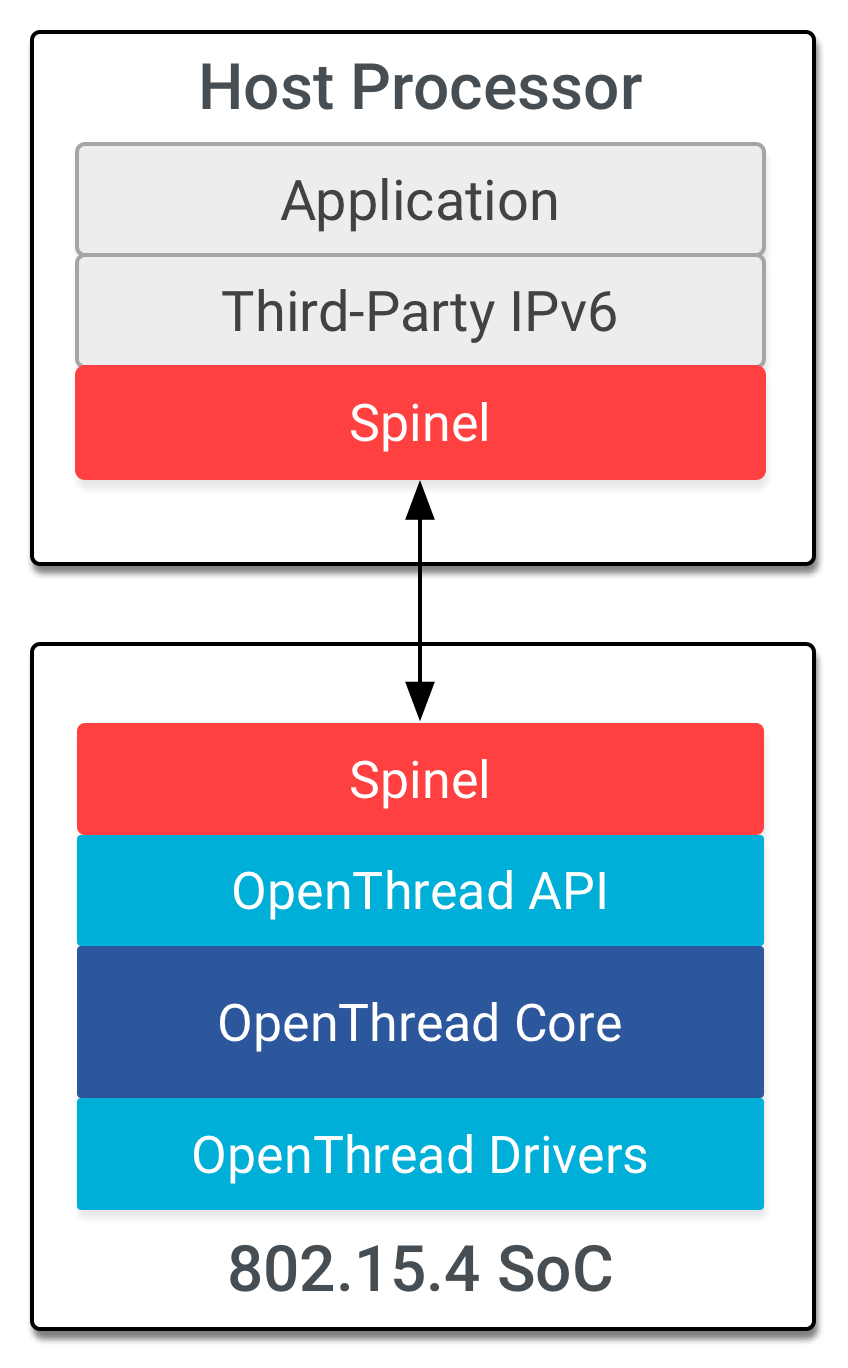
\includegraphics[width=5cm]{img/ncp-design.png}}
    \hfill
    \subfigure[Radio Co-Processor]{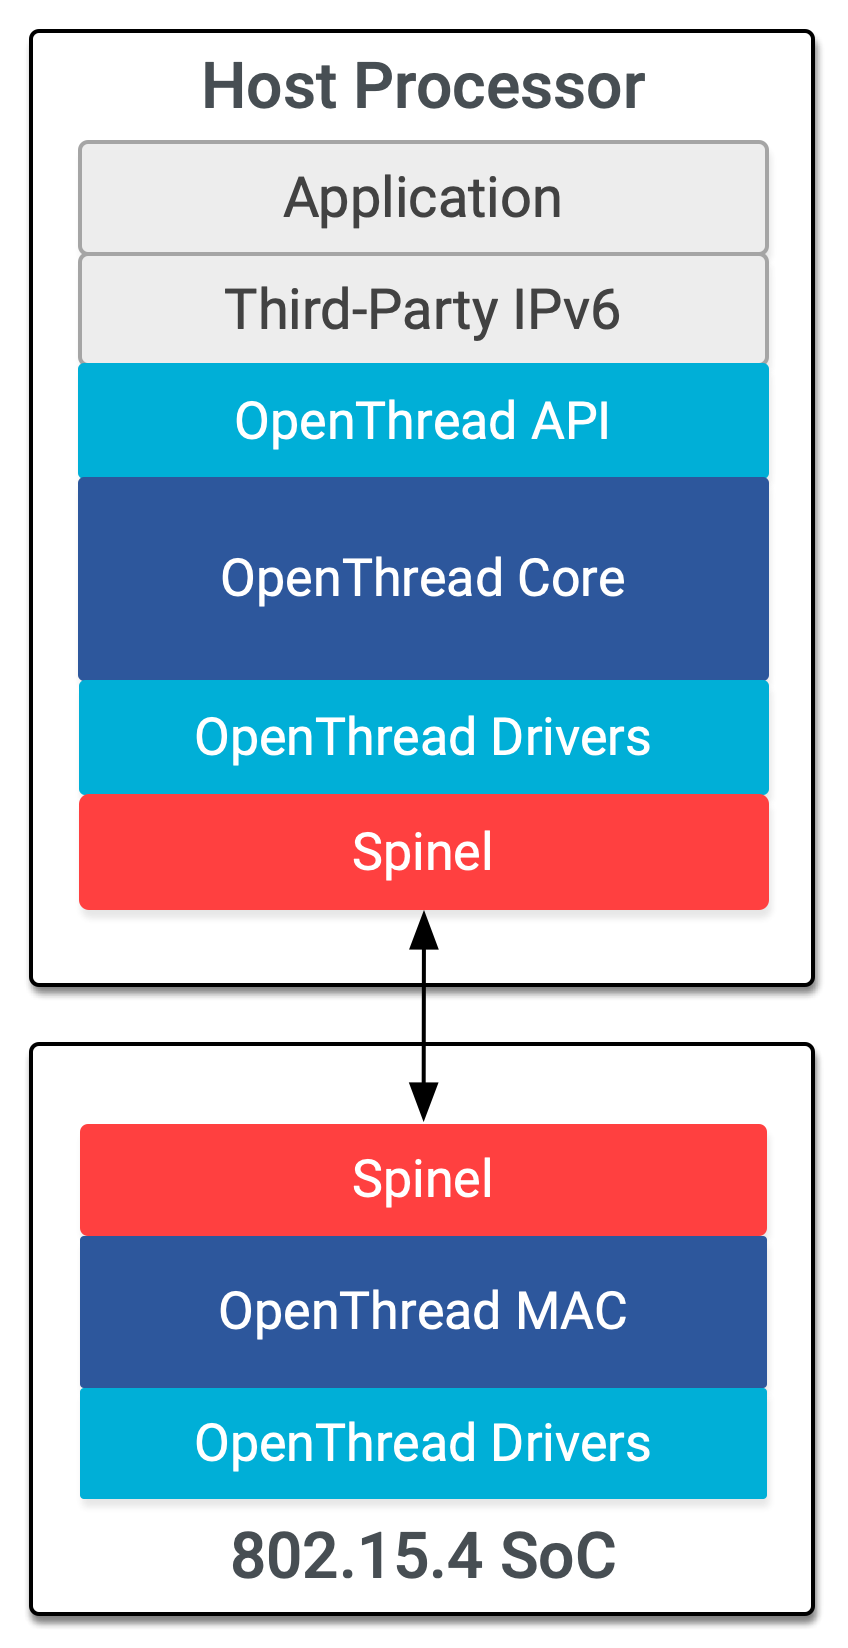
\includegraphics[width=5cm]{img/rcp-design.png}}
    \caption{Network Co-Processor vs. Radio Co-Processor}
    \label{fig:ncp}
    \cite{platforms}
\end{figure}

\subsubsection{Network Co-Processor}
One of these solutions is the \textit{Network Co-processor} (\textbf{NCP}), which is shown on the left side of the Figure \ref{fig:ncp}. The developers are using this design, when offload of the main resource (\textit{Host processor}) is required to save energy, as it allows to run the processor in \textit{idle} state or even keep it asleep. It may also be the case that some resource-intensive activity makes it important not to overload the processor, such as processing an image from a camera. In this case, the Thread API and the layer needed to construct the communication principle (\textit{Thread Core}) will run together with the physical layer of the Thread Radio on a much lower power, separate processor. The Host processor and the Co-Processor can communicate via UART, SPI or USB. In the diagram, this communication is implemented in the "Spinel" layer, which is a protocol developed by Google specifically for this task. This protocol is described in this \href{https://datatracker.ietf.org/doc/html/draft-rquattle-spinel-unified}{documentation}\cite{SpinelDoc}. From the image on the left, it can be concluded that the Host will only run IPv6 management and the application.

\subsubsection{Radio Co-Processor}
In this case, which called \textit{Radio Co-Processor} (\textbf{RCP}), only a minimal communication layer of Thread MAC and the physical driver are running together. This has the advantage that all OpenThread-related layers are located on the much more powerful Host processor. The biggest benefit is, when the Thread API or Thread core changes, the device is not needed to flash with the new firmware. As in the previous case, it communicates via some sort of serial communication.

\subsection{The Co-Processor design used for the implementation}
Based on the above, I created my own Border Router using NCP in the first version, but due to the continuous rapid changes in OpenThread, a direction is emerging that the RCP design will prevail in the development phase. It is currently the only one supported by Google, so I have continued development and hardware design in that direction. 

\subsection{Raspberry Pi HAT - Border Router}
\subsubsection{Requirements}
I created the Border Router with a Raspberry Pi 4 and on it a self designed and programmed HAT. The word \textbf{HAT} comes from \textit{Hardware Attached on Top}. Since 2014, Raspberry Pi has been developing the HATs \href{https://github.com/raspberrypi/hats}{GitHub}\cite{HATSGitHub} repository. The idea behind which is to create different devices using the Raspberry Pi Model B pin header. This consists of 40 pins since the second series and its basic layout has not changed since then. Over the years, as more and more complex Broadcom chips appear in the Raspberry, more and more functions are available on a single pin header's pin. On these HATs if I place an EEPROM, which is communicating via I2C, than the Raspberry Pi can configure the GPIO pins at boot time based on the data in this memory.
It is a basic requirement that two pins (GPIO 0 and GPIO 1) dedicated to the I2C EEPROM can not be used for any other task. Furthermore, two other basic requirements are set by the developers. One is that if it is possible to connect the power supply from the HAT, it must be protected from back powering by an \textit{ideal diode}. If the power supply is connected through the Raspberry's power port, it can cause damage to the power module because of the different voltage levels. The third basic requirement is that certain pins must be protected from short-circuiting, as these are configured to output during boot time in older versions, as they are used for boot time signalling.
A device can only be described as a HAT if:
\clearpage
\begin{itemize}
    \item it satisfies the three basic requirements,
    \item it has an I2C EEPROM containing real, processable data and this is soldered on the HAT,
    \item it can connect to the Raspberry with a 40 pin spike line,
    \item it must follow the mechanical specification (given size and hole diameters),
    \item it has at least 8 mm distance between the two PCBs,
    \item it is capable of supplying at least 1.3\,\si{\ampere} of continuous current through the 5\,\si{\volt} pin.
\end{itemize}
During the design process I followed these guidelines, therefore my Thread Border Router could be called a HAT.

\subsubsection{EEPROM and stored data}
For EEPROM I chose a 256 \si{\kilo}Byte memory from OnSemiconductor\newline \textbf{CAT24Cxx}, because it has hardware write protection for the entire memory area, unlike the same series of ICs from Microchip. Thus, on the custom hardware a jumper must be removed when writing, so that the user can not accidentally overwrite the EEPROM contents.
This repository contains target-specific programs for writing EEPROM and generating EEPROM contents. To make configuration easier, it is needed to specify in a text file which GPIO pin and which function want to be configured, which can be input, output or an alternative function. These can be found in the documentation of the specific Raspberry Pi BCM chip. Furthermore, it is possible to add pull-ups or pull-downs to the input configured pins.
\begin{figure}[!htb]
    \centering
    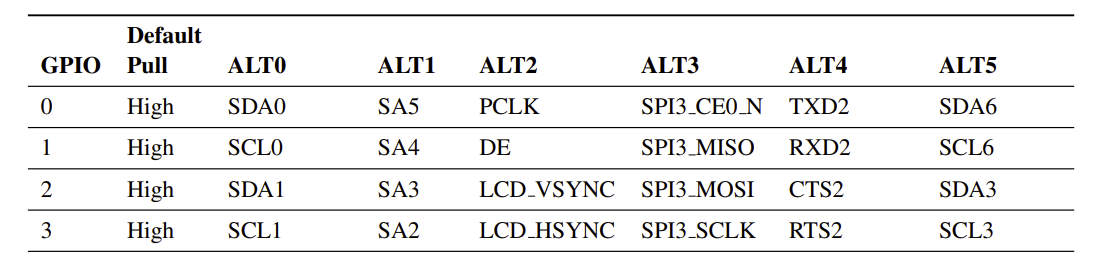
\includegraphics[width=\textwidth]{img/bcmgpio.png}
    \caption{The first four GPIO functions of the Raspberry Pi 4}
    \label{fig:gpios}
    \cite{RaspberryBCM}
\end{figure}
The Raspberry Pi 4 is built with a BCM2711 chip and the functions of the first four GPIO pins are shown in Figure \ref{fig:gpios}. From this table, it can be seen that if these are configured as ALT0 function pins, two I2C peripherals are obtained. In the other case, if an UART peripheral is needed with data flow control, it should be chosen to be ALT4 function.
If the memory is filled with valid data, the next time during the boot process of the Raspberry the data will be automatically read and the pins are initialized accordingly. It is important to note that there is a config.txt file in the \textit{/boot} partition where special peripherals are needed to be enabled with a program, which called \textit{dtoverlay}. For example, the dtoverlay program can enable the uart3 peripheral with flow-control with this line:
\begin{center}
    dtoverlay=uart3, ctsrts
\end{center}


\subsection{Raspberry Pi HAT - Border Router Design}
\begin{figure}[!htb]
    \centering
    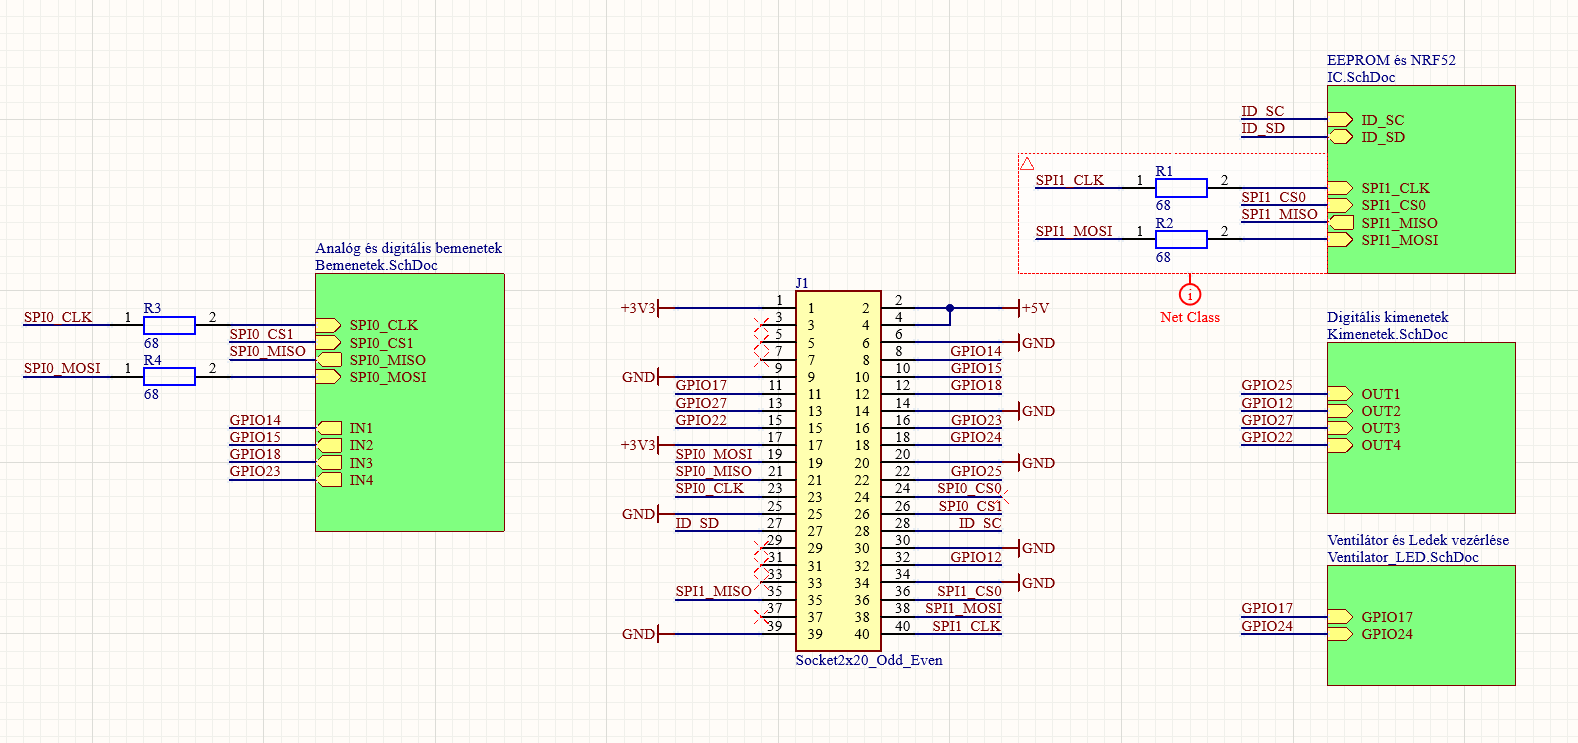
\includegraphics[width=\textwidth]{img/rpischematics.png}
    \caption{Raspberry Pi HAT wiring diagram}
    \label{fig:Schematics}
\end{figure}
\noindent
My goal was to develop a device that would be a transition between a Proof-Of-Concept and a final product. The hardware design was made with Altium Designer, because it is one of the most widely used design tool. As the Figure \ref{fig:Schematics} shows, the schematic can be divided into four different parts. Inputs are on the left side, where four digital and two analogue inputs are located. These inputs are protected against overvoltage (up to 7\,\si{\volt}), so that the digital inputs tolerates 5\,\si{\volt} TTL signals or in case of a bad connection the higher voltage can not damage the input/output pins. The analogue inputs measure the connected voltage in the range from 0 to 3.3\,\si{\volt}, thus offering additional applications. Since the Broadcom chip used by the Raspberry Pi does not have an analog-to-digital converter, the measurements are made by an external Microchip SPI-communicating IC for this, which was available compared to its I2C counterpart in the middle of the current chip shortage. In the middle there is the 40 pin socket and the connection for those. In the upper right corner the I2C EEPROM and an nRF52840 connected via SPI. To reduce the crosstalk, the design contains a 68 ohm resistor on each of the SCK and SDO lines to increase the rise/fall times of the changes. The digital outputs block is in the centre right, which have signal levels of 0 and 3.3\,\si{\volt} and are also protected from overvoltage and short circuit from connecting outputs due to bad wiring. The inputs, outputs, 5\,\si{\volt} and ground power lines are available through 50 mil grid spacing terminal blocks on the PCB. And in the lower right corner is shown the control block for the five LEDs and two fan outputs on the PCB. These can be switched on and off by 3.3\,\si{\volt} and the brightness and rotation speed can be controlled by PWM. The LEDs are for design purposes only, while the fans are used to protect the device from overheating. A detailed breakdown of the green blocks is shown in Figure \ref{fig:borderrouterbemenetek}-\ref{fig:borderventiled}.
\begin{figure}[!htb]
    \centering
    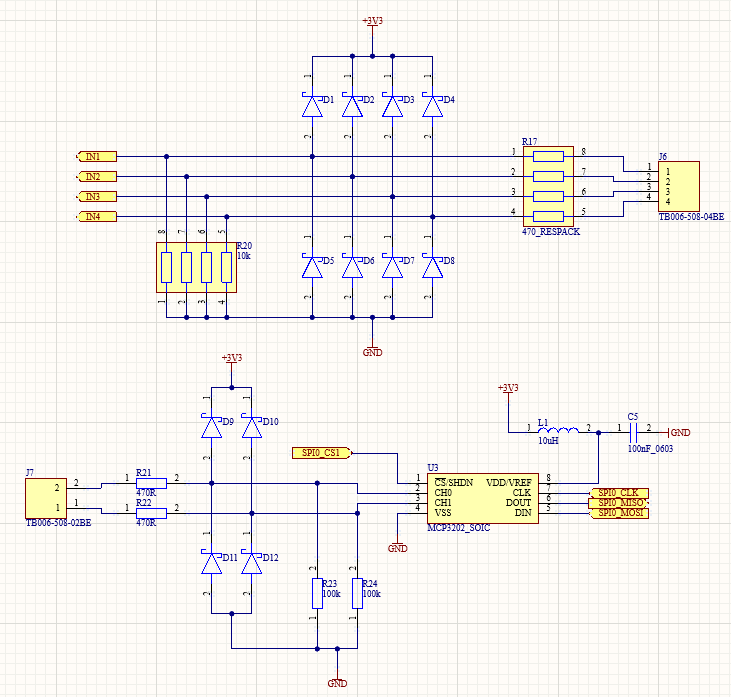
\includegraphics[width=\textwidth]{img/bemenetekrpihat.png}
    \caption{Raspberry Pi HAT inputs}
    \label{fig:borderrouterbemenetek}
\end{figure}
\begin{figure}[!htb]
    \centering
    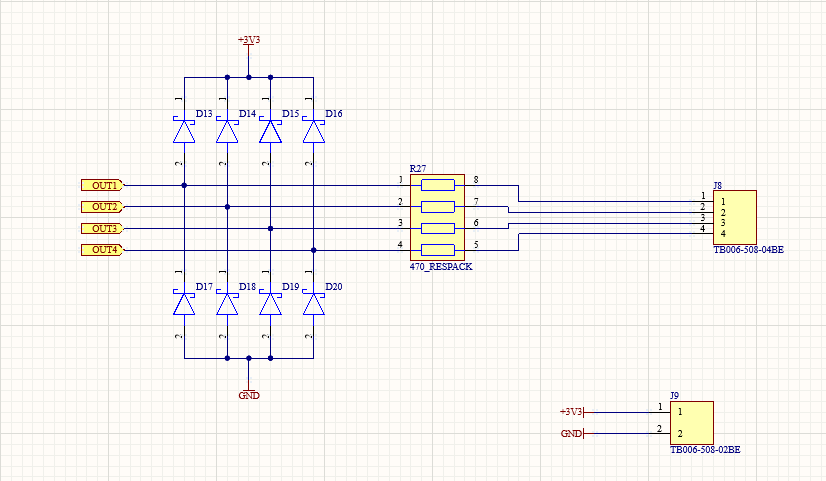
\includegraphics[width=\textwidth]{img/kimenetekrpi.png}
    \caption{Raspberry Pi HAT outputs}
    \label{fig:borderrouterkimenetek}
\end{figure}
\begin{figure}[!htb]
    \centering
    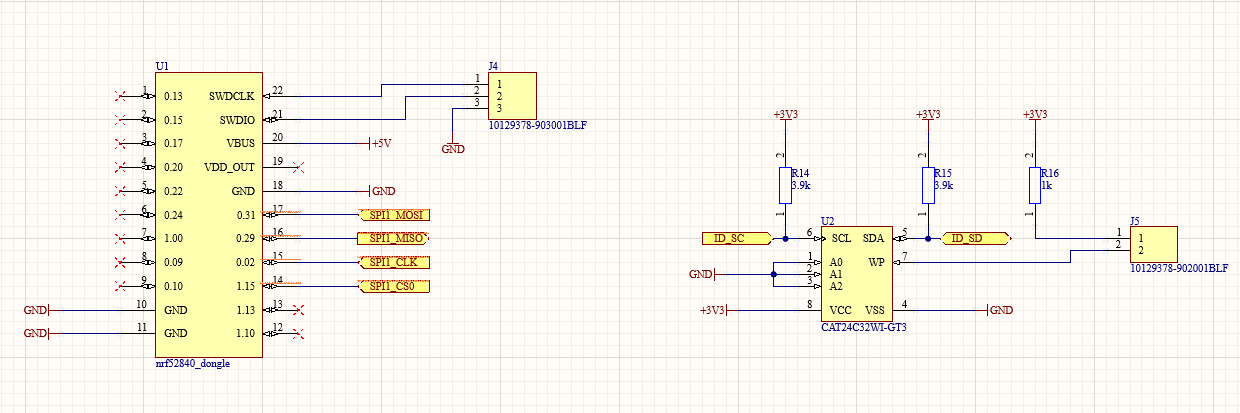
\includegraphics[width=\textwidth]{img/eeprom.png}
    \caption{Raspberry Pi HAT Integrated Circuits}
    \label{fig:borderrouterick}
\end{figure}
\begin{figure}[!htb]
    \centering
    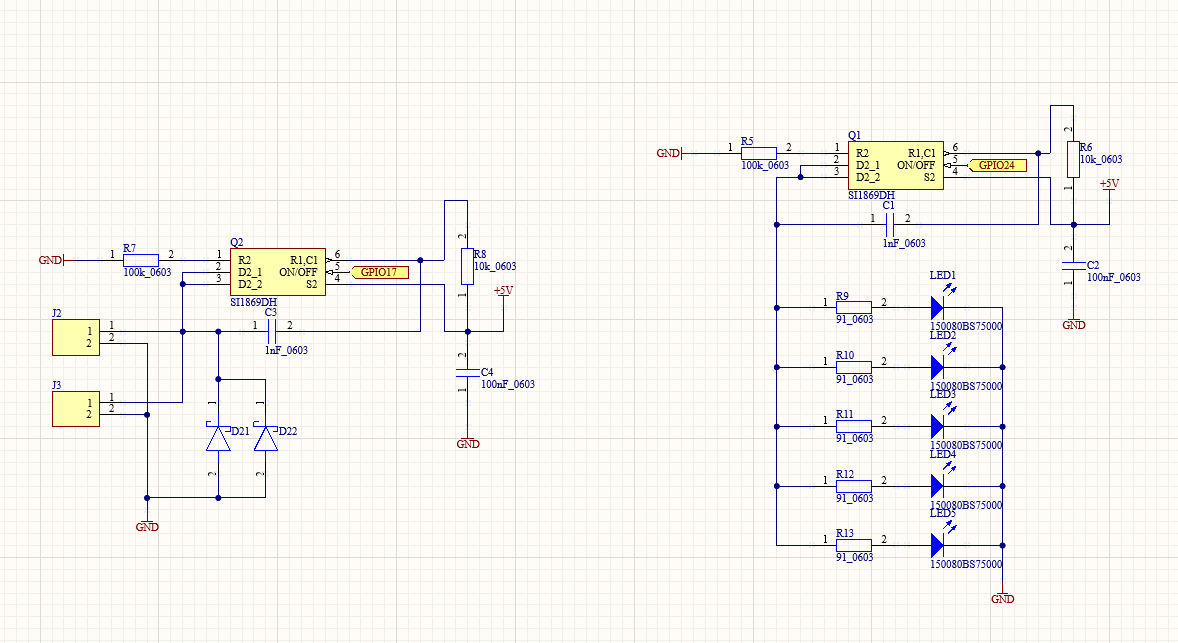
\includegraphics[width=\textwidth]{img/ickrpihat.png}
    \caption{Raspberry Pi HAT LED and fan controller}
    \label{fig:borderventiled}
\end{figure}
\newline
Figure \ref{fig:3drpi} shows the finished PCB plan in 3D view.
\begin{figure}[!htb]
    \centering
    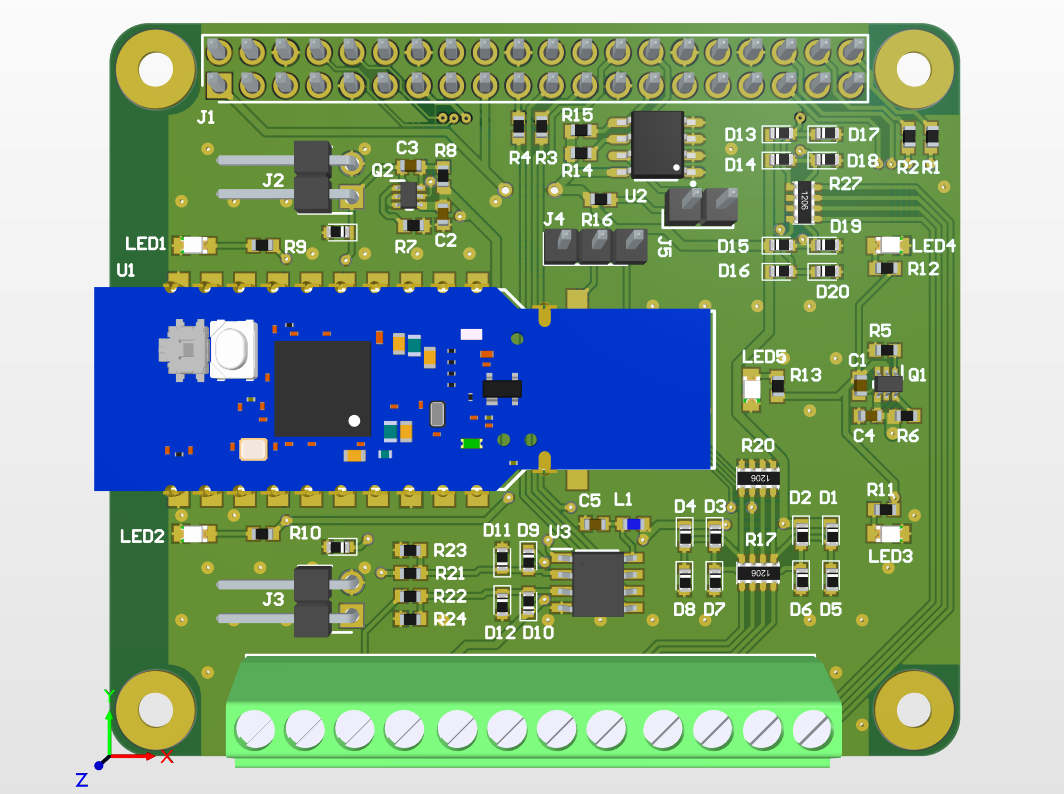
\includegraphics[width=\textwidth]{img/rpi3d.png}
    \caption{Raspberry Pi HAT in 3D viewer}
    \label{fig:3drpi}
\end{figure}


\subsection{Border Router housing}
It was important to make a housing in which I can place the Border Router, thus protecting the device from mechanical damage. The model of this device was made in AutoCAD Inventor.
The model includes two 5\,\si{\volt} brushless DC fans (short \textbf{BLDC}) to reduce the Raspberry Pi temperature by blowing air through the housing. The Ethernet and USB Type C ports is cut out, as the device can only be powered via USB port and the Ethernet port is the only way to connect to the home network. There is also space for access to the screw terminal ports, so the user can easily access the the 5\,\si{\volt} power supply, inputs and outputs with a flat-head screwdriver. On the Figure \ref{fig:3dbd} there is the housing model in 3D viewer.
\begin{figure}
    \centering
    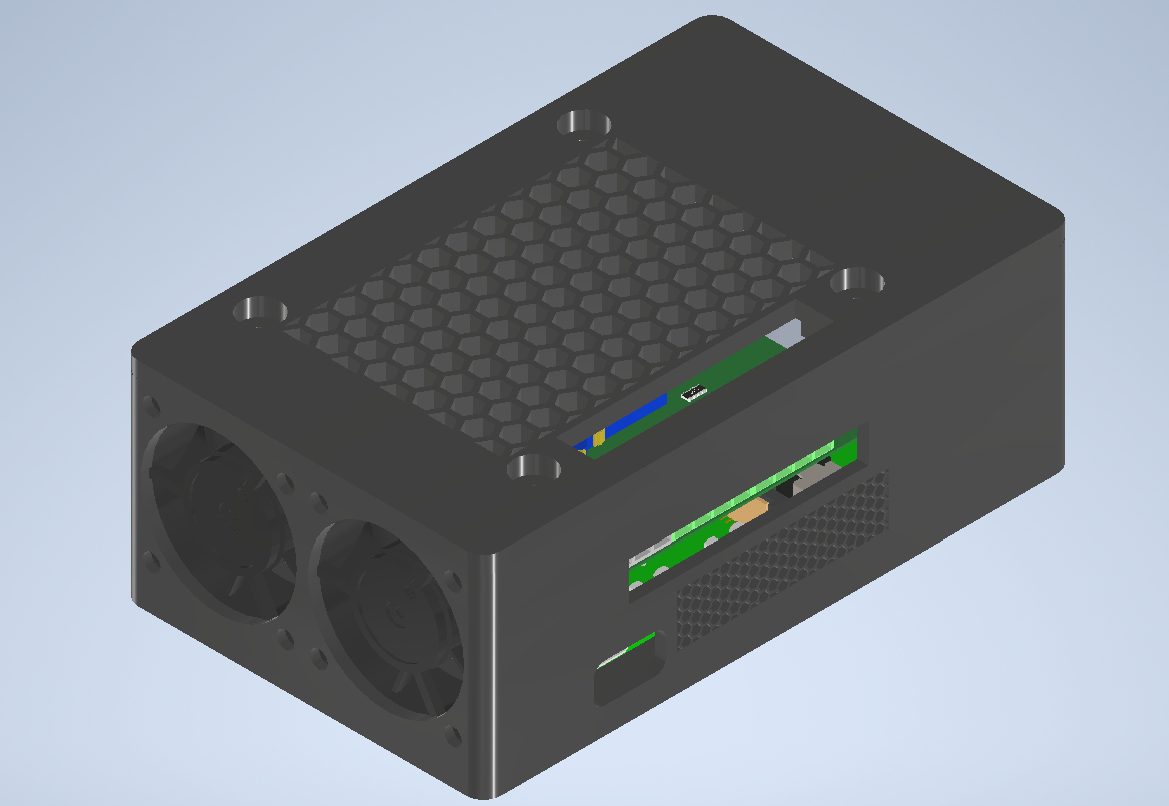
\includegraphics[width=\textwidth]{img/3ddoboz.png}
    \caption{Border Router housing in 3D viewer}
    \label{fig:3dbd}
\end{figure}


\subsection{Border Router software}
\subsubsection{nRF52840 RCP software}
For the Radio Co-Processor I use the package developed by OpenThread for nRF52840 and compiled it to the SPI pins. I modified the SPI pins in the dedicated header file, called "transport-config.h". The software is available at this \href{https://github.com/openthread/ot-nrf528xx}{GitHub repository}\cite{OTBR}. For the SPI communication, a total of six pins are required, four of for the SPI communication, one pin is tied to the hardware RESET pin of the microcontroller and one pin is held up for interrupt signalling. The last two pins are optional according to the documentation and if no interrupt signal is used, than the communication would be slowed down because the Host device would have to make continuous requests. In reality, the situation is different, since the code contains a section that if one of the two optional pins is missing, the program will return with an error code. Since the hardware RESET pin of the Dongle device is not hardwired, but is tied to a specific button, so SPI communication is not possible. So I switched to the much slower UART communication, which requires four pins, two data pins (Rx, Tx) and two signals (CTS, RTS). After uploading the code, the device was ready to communicate. It is worth noting that there are some pins that can only be used for low frequencies (10\,\si{\kilo\hertz}), as they run on-chip next to the RF module, so the manufacturer does not guarantee immunity to crosstalk.

\subsubsection{Raspberry Pi - OpenThread official software}
OpenThread provides a Raspbian-based GNU/Linux distribution to implement the the Border Router, but it is also available as a separate group of applications that the developer has to install. After the installations, three programs are available in the operating system, \textit{otbr-agent} (from OpenThread-BorderRouter name), which performs communication with the RCP via SPI, UART or USB, depending on the build. Closely related to this is the avahi-daemon, which resolves the Network Interfaces. The \textit{otbr-agent} makes a \textit{Wireless Personal Area} interface, namely \textbf{WPAN0}. If the \textit{ifconfig} program is used, than this program lists this interface in the result list. The third program is \textit{otbr-web}, which provides a configuration rudimentary web page at localhost address on port 80, where the user can create a Thread network, initiate a connection and view the before created Thread network with the available devices on this networks on a visualisation page. To connect an optional fourth program, which is called \href{https://github.com/openthread/ot-commissioner}{\textit{ot-commissioner}}\cite{OTCOMMISSIONER}, is required. Before use this have to be compiled, because this repository contains only the source code. Since the user or the developer can reach the Thread network over the internet via a website, this device act as a Border Router.

\subsubsection{Border Router scripts for other functions}
After boot time, when the otbr-agent software is available, I am using a Python script to create a Thread network by calling \textit{ot-cli}. With this program over the Linux kernel I can manage the Co-Processor, for example I can create my own Thread network, join an existing network or even map the network. A Python script manages the lights and the fan, that script constantly monitors the processor temperature and if it rises towards 60\,\si{\celsius}, the fan starts to spin up under the control of a 50\,\% duty cycle control signal. If it rises even further, the duty cycle changes on a linear scale up to 100\,\%, which is reached at 70\,\si{\celsius}.

\subsection{Summary of the Border Router}
In this section I presented the Border Router, which I designed. I showed the differences between NCP and RCP and the rules of HATs, which were necessary to develop this board. I showed the functionalities of this board and made a solution to set up a Thread network.

\section{Graphical User Interface}

\subsection{Introduction}
My goal was to make an easy to use interface, where the possible users of these devices can access their network and can manage their devices efficiently. On the other hand this solution gives an informative, nice looking visualisation page. Because Thread Network can be connected to the internet, I chose a Webpage as a GUI to use.

\subsection{Programs used for the website}
The interface is implemented with a webpage, which I create with \textit{Bootstrap CSS}, \textit{HTML} and on the client side I use \textit{JavaScript} to check the integrity of the data. On the server side, I use \textit{FastAPI} as backend, which is one of the fastest Python frameworks currently available. Thanks to the Python language
\begin{itemize}
    \item it can be developed quickly, 
    \item because of the python's syntactics is less chance of bugs from typos,
    \item it is easy to learn,
    \item it can be developed in relatively short code, avoiding unnecessary code duplication.
\end{itemize}
\clearpage
\noindent
Furthermore, FastAPI is characterized by
\begin{itemize}
    \item it is robust, produces automatic documentation and is easy to debug,
    \item it is based on JSON schema and OpenAPI.
\end{itemize}
I run the website on a \textit{Asynchronous Server Gateway Interface} (short \textbf{ASGI}) web server which called \textit{Uvicorn}. Essentially, this creates the connection between the backend and the web server. That is, in the event that an HTTP request is received from the client, the web server will signal this to FastAPI. All communication between the program and the server will be done in a Python Dictionary format, which is a data structure. A Dictionary is similar to the JSON data format, which is stored as text, whereas a Dictionary is a memory object.
I implement the dynamically changing web page elements with \textit{Jinja template}. This program does the processing of the data from the Dictionary objects and pastes it into the appropriate location into the html page. This template language also contains conditional branching and foreach cycles.


\subsection{Database}
Before I get to the backend, I would like to introduce the database model, which I designed.
\begin{figure}[!htb]
    \centering
    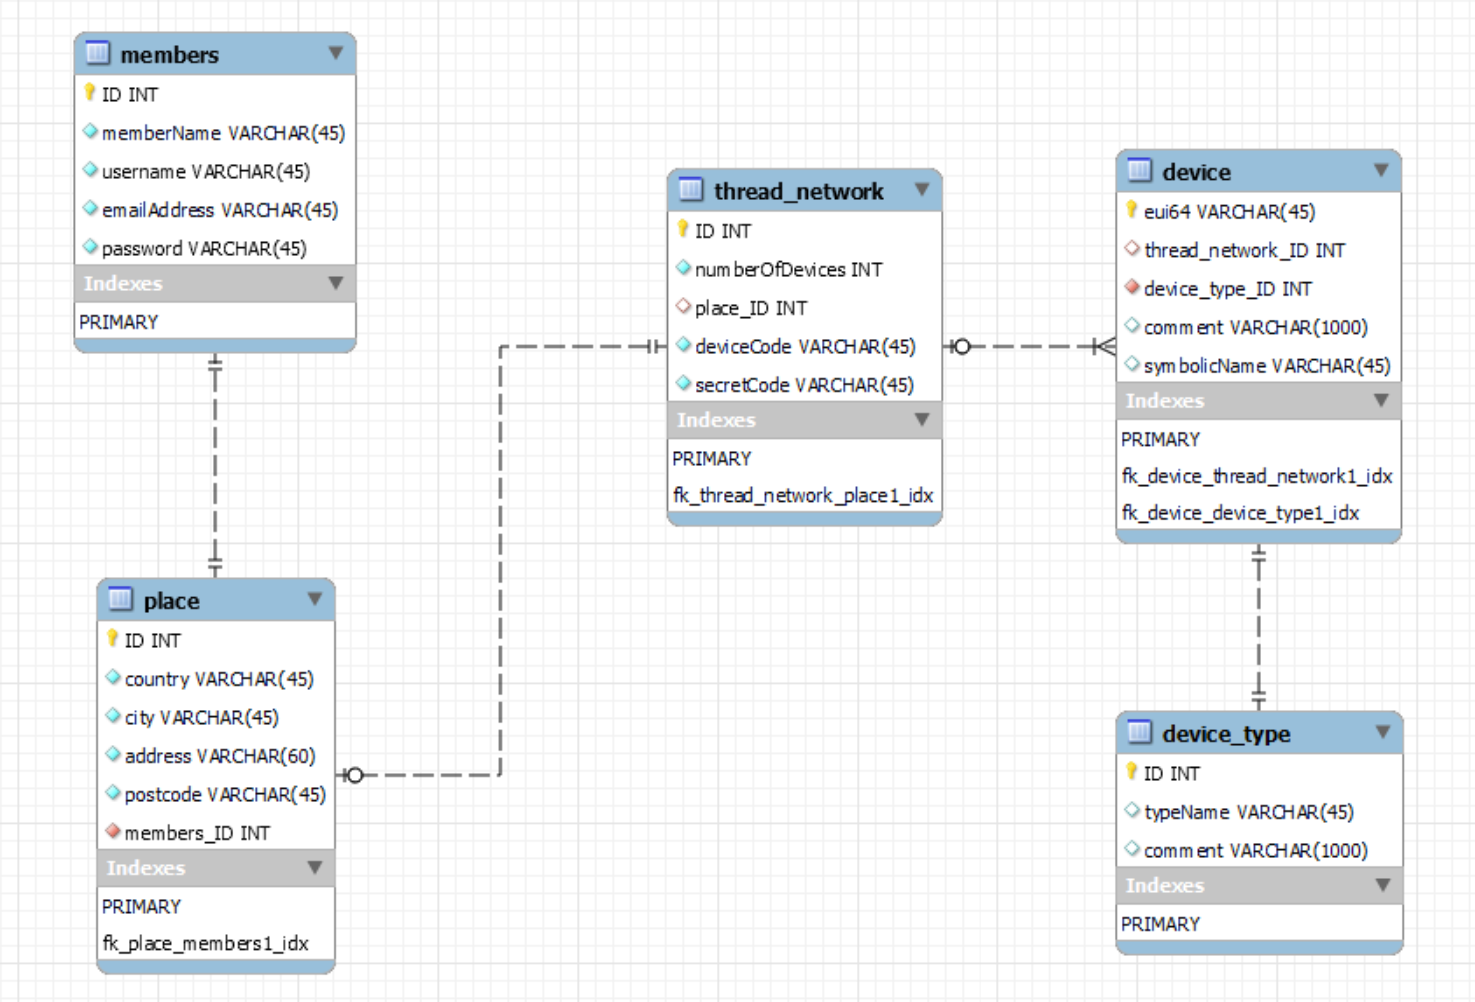
\includegraphics[width=\textwidth]{img/adatbazis.png}
    \caption{The database model}
    \label{fig:database}
\end{figure}

\subsubsection{Users or members}
The data is stored in a \textit{MariaDB} database, which is an Open-Source version of MySQL. Figure \ref{fig:database} shows that there is a separate table for users starting from the top left corner.
For each user, I associate an ID that is automatically incremented and that corresponds to the primary key. A user also has a name, surname combination and an email address, each of which forms a separate column. For faster login, I associate a username with the previous ones and of course a password that the user can enter.

\subsubsection{Place}
I designed my Thread network so, that only one Thread network can exist in one home. I think during this development, more than 16,000 devices are enough for a house. So I store where this apartment is located, geographically in this table. This table already contains an external key, because a house can belong to a user and this connection is implemented by a one-to-one connection.

\subsubsection{Thread network}
Only Border Routers can make Thread networks in this development. All networks should be pre-populated in the database, so that when a user gets access to one, it just have to be registered to the home. Each network has an ID which is also automatically incremented and this is also the primary key. A column contains the number of device connected to a the network, purely for statistical reasons and to deal with the case that someone wants to connect more than 16,000 devices. The registration process is such that each device has a private name, which I call deviceCode in the table and a secret password, which I call secretCode. These can be supplied on a piece of paper with each device.


\subsubsection{Device type}
Each device type has an ID, which is also an automatically incremented primary key and two additional columns. One of these stores the name of the device type, such as the Thread router and optional lamp switch as Blind Access Point described later and the associated comment. In the comment column I store a basic configuration of the device as text. As JSON is easy to handle inside Python, I put the data into a JSON file and convert it to text.
\begin{lstlisting}[language=Python]
    BLIND_ACCESS_POINT_DEVICE_TYPE_STRUCT = {
        "isLampConnected": False,
        "lampstate": False,
        "isExtensionBoardConnected": False,
        "whichExtendedActive": "00000"
    }
\end{lstlisting}

\subsubsection{Devices}
Each device has a unique identifier, similar to the MAC address from the Internet world, only unlike that it is a 64-bit number. This is the eui64 identifier, which I described in an earlier section. Since it is unique for each device I use it as the primary key. Since the devices are also provided by the manufacturer and they do not know which Thread network they will be connected to, the second column in this table will be initialized with NULL, so it is allowed to have the external key take NULL value. This is indicated by the empty red circle. Also the device must have a type and the comment field must be copied to the device with the default settings. This is necessary because if it is a lamp switch then each lamp must have a unique state. This table has a one-to-many relationship with the Thread Network table, since multiple devices can be connected to a network.


\subsection{Backend and website design}
\begin{figure}[!htb]
    \centering
    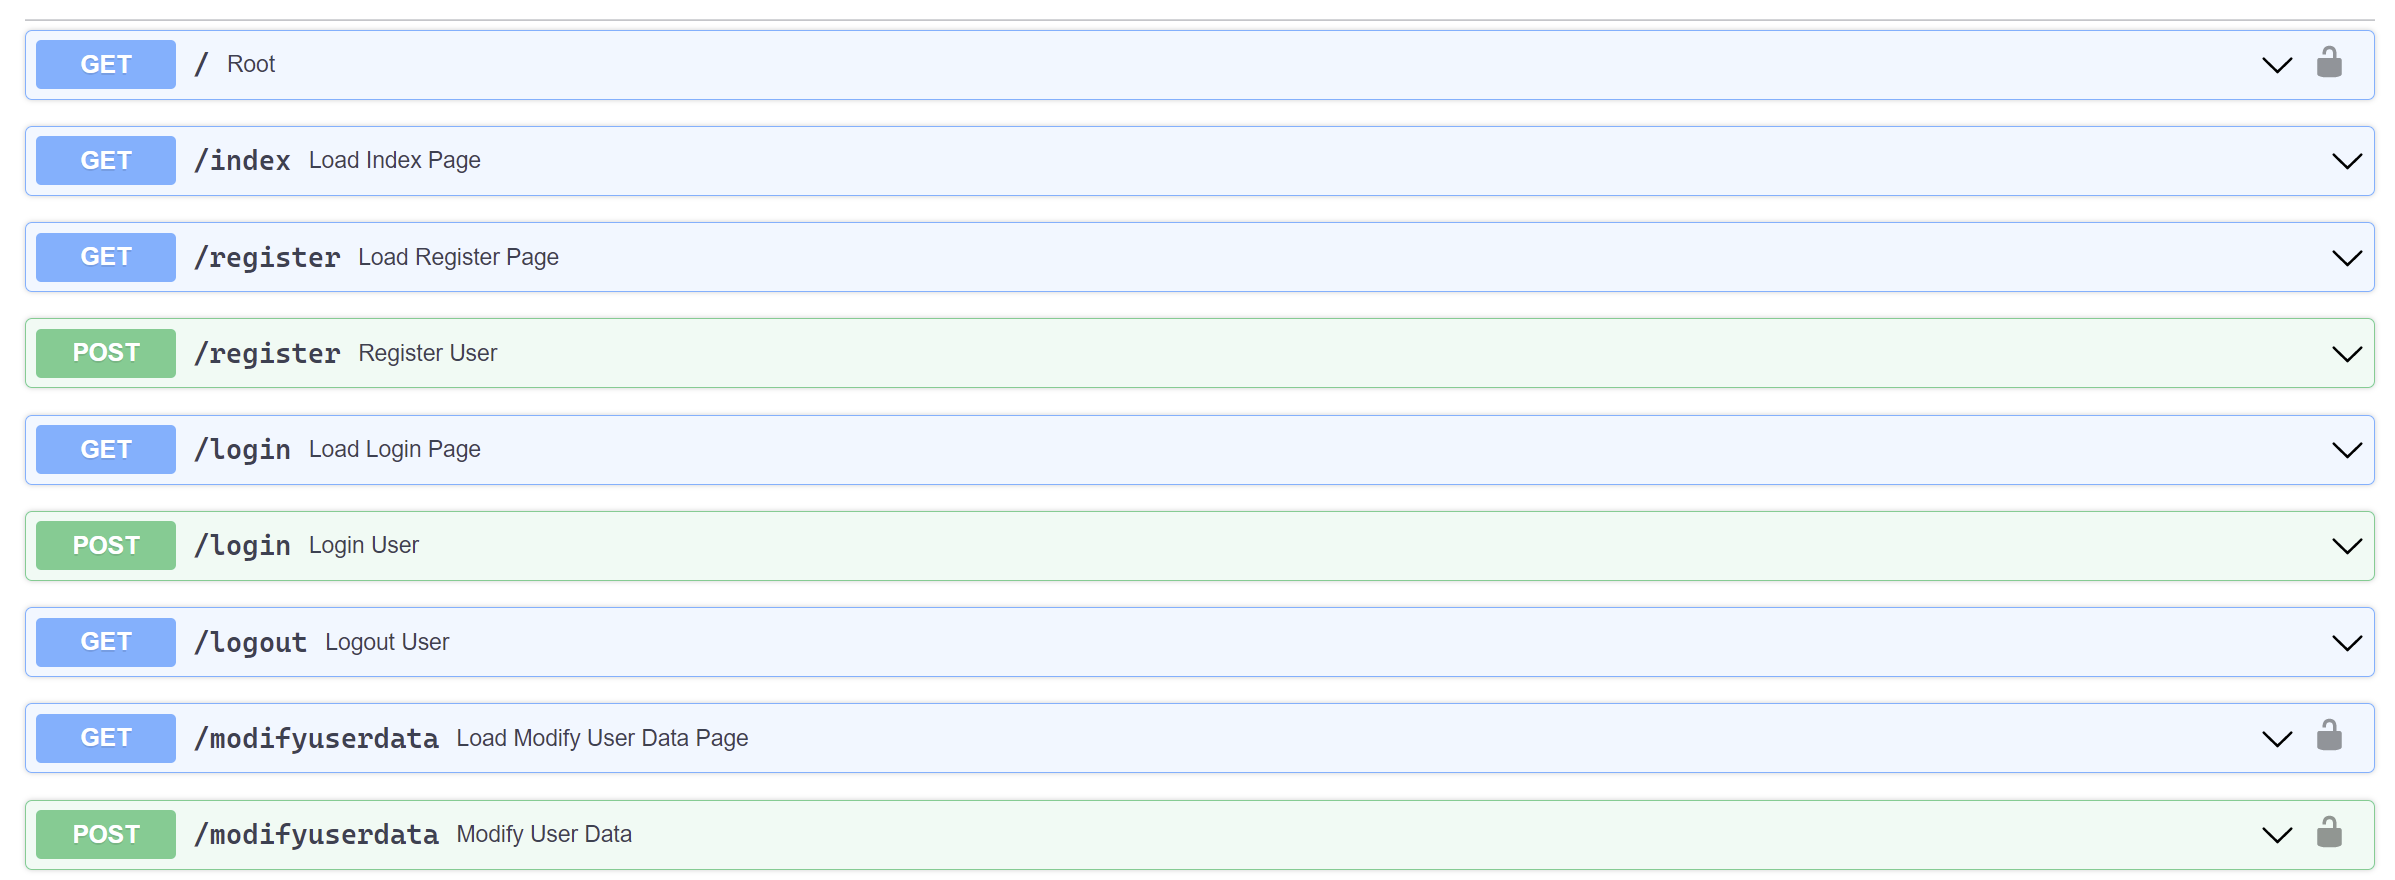
\includegraphics[width=\textwidth]{img/backend.png}
    \caption{Automatic documentation of FastAPI}
    \label{fig:backend}
\end{figure}
\noindent
FastAPI, as I write in the initial listing, produces automatic documentation that the developer can access under "/docs". Part of this documentation is shown in Figure \ref{fig:backend}. On the left side, this documentation shows what queries a particular routine is called for. For example, a registration GET request directs the user to a registration page where HTML forms are found. In the case where all fields are filled in and valid information is provided, a POST request is sent to the same address. Three JavaScript function check the data integrity in the frontend, because of the crash protection and only if all fields are filled in and valid, than the backend executes the query. After a POST request, the data is downloaded from the database and the webpage redirects the user to a feedback page where the user gets informed about the result of the registration process, which may be successful or not, because the passwords do not match or a user already exists.\newline
Where there is a padlock on the right, the website can only be accessed after authentication (\textit{login}). I based the login on the industry standard OAuth2. However, the important information is that the authentication can be done within the HTTP protocol header or with a Cookie. I choose the latter solution and so after login I store the username of the logged-in person and the expiration date of the cookie, which is 24 hours in the browser with a secret key using SHA256 encryption. Before decryption or after decryption, a JSON format will be obtained and that is why it is called \textit{JSON Web Token} or \textbf{JWT}.


\subsection{Frontend}

\subsubsection{Services available to the authenticated user}
\begin{figure}[!htb]
    \centering
    \subfigure[Before logging in]{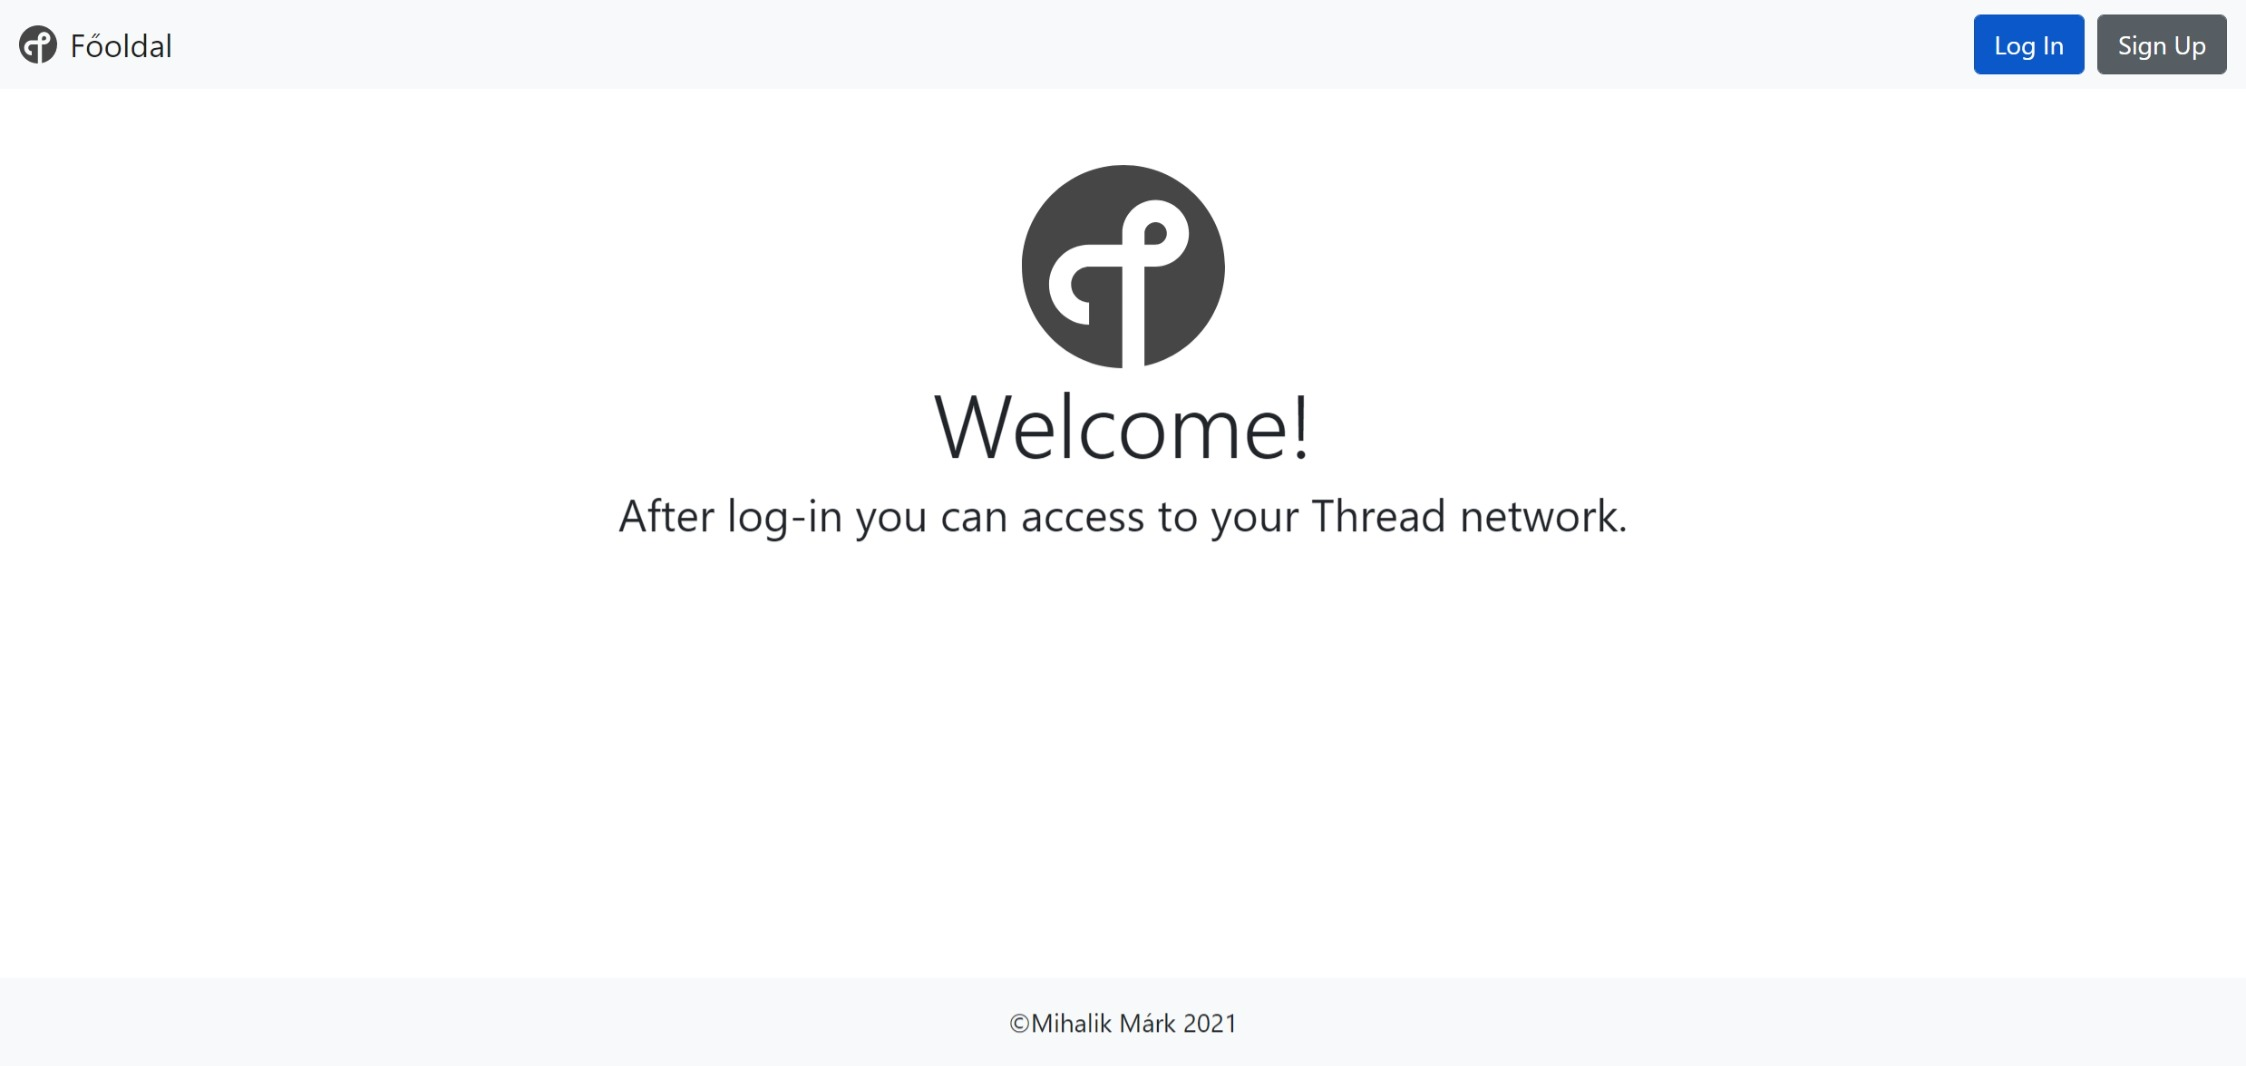
\includegraphics[width=\textwidth]{img/bejelentkezeselott.jpeg}}
    \subfigure[After logging in]{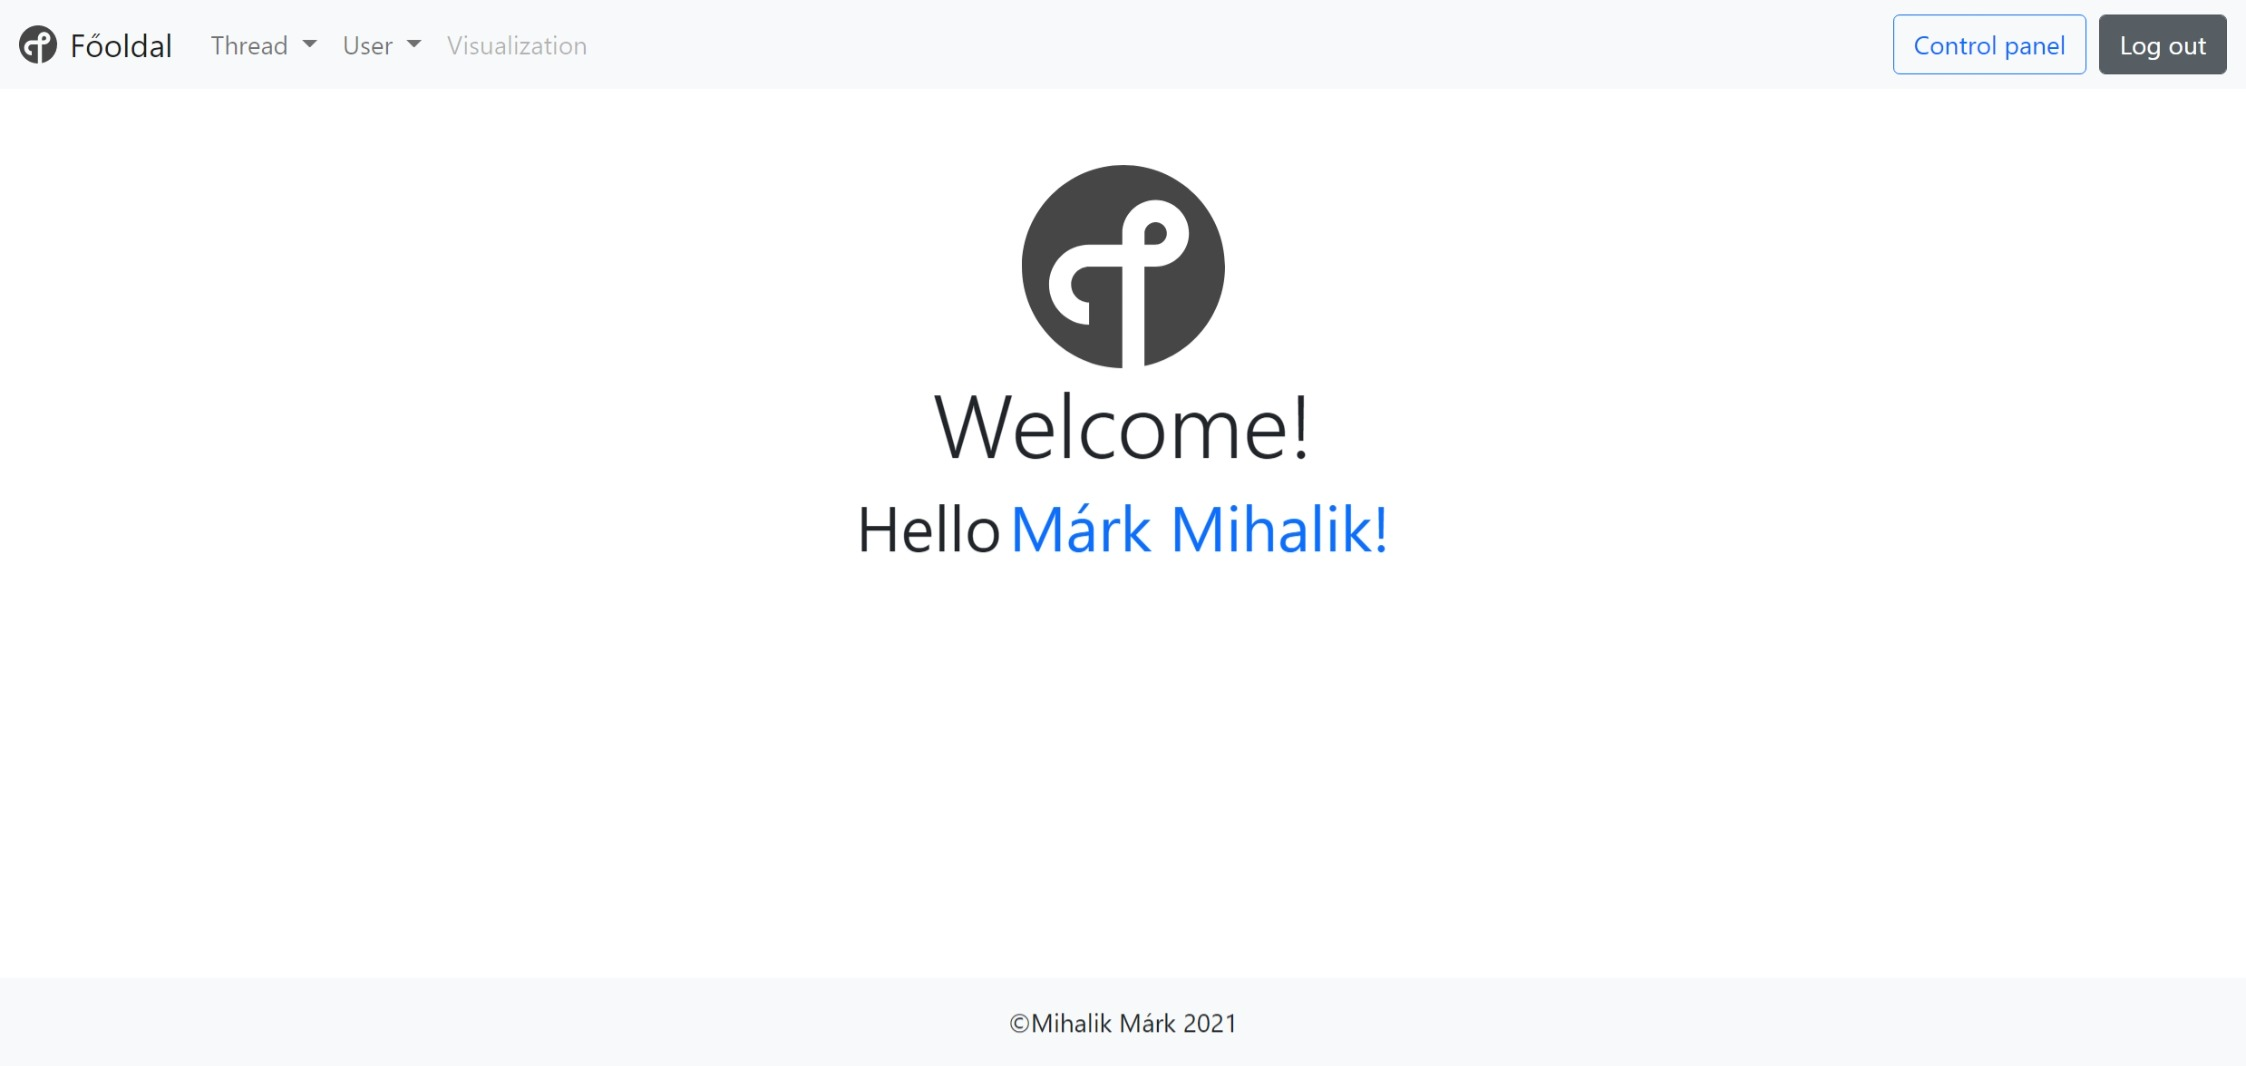
\includegraphics[width=\textwidth]{img/bejelentkezesutan.jpeg}}
    \caption{The main pages of the Webpage}
    \label{fig:welcomepage}
\end{figure}
Figure \ref{fig:welcomepage} shows two pictures of the changes that are available to the user before and after logging in. In the header, there is a change, as dropdown menus appear in the previously empty spaces. The first of these menus is Thread, where the network can be added or possibly deleted. The second dropdown menu is where the user can add location to the personal information or if this information already exists, then the user has the possibility to change it. On the right side, the Login and Register buttons changes after the Log In, as they have been replaced by two other functions, one for the Control Panel and the other for Log Out. 

\subsubsection{Control Panel}
Clicking on this button makes available to the user the devices in the database that belong to the user. As shown in Figure \ref{fig:controlpanel}, there are currently two devices in the database and both devices are Blind Access Points. On one of them the relay that switches the light is active and on the other one it is not, these are indicated by the yellow and white background. The lamps can be removed by software in case, when this device only want to be used as a router or REED.
\begin{figure}
    \centering
    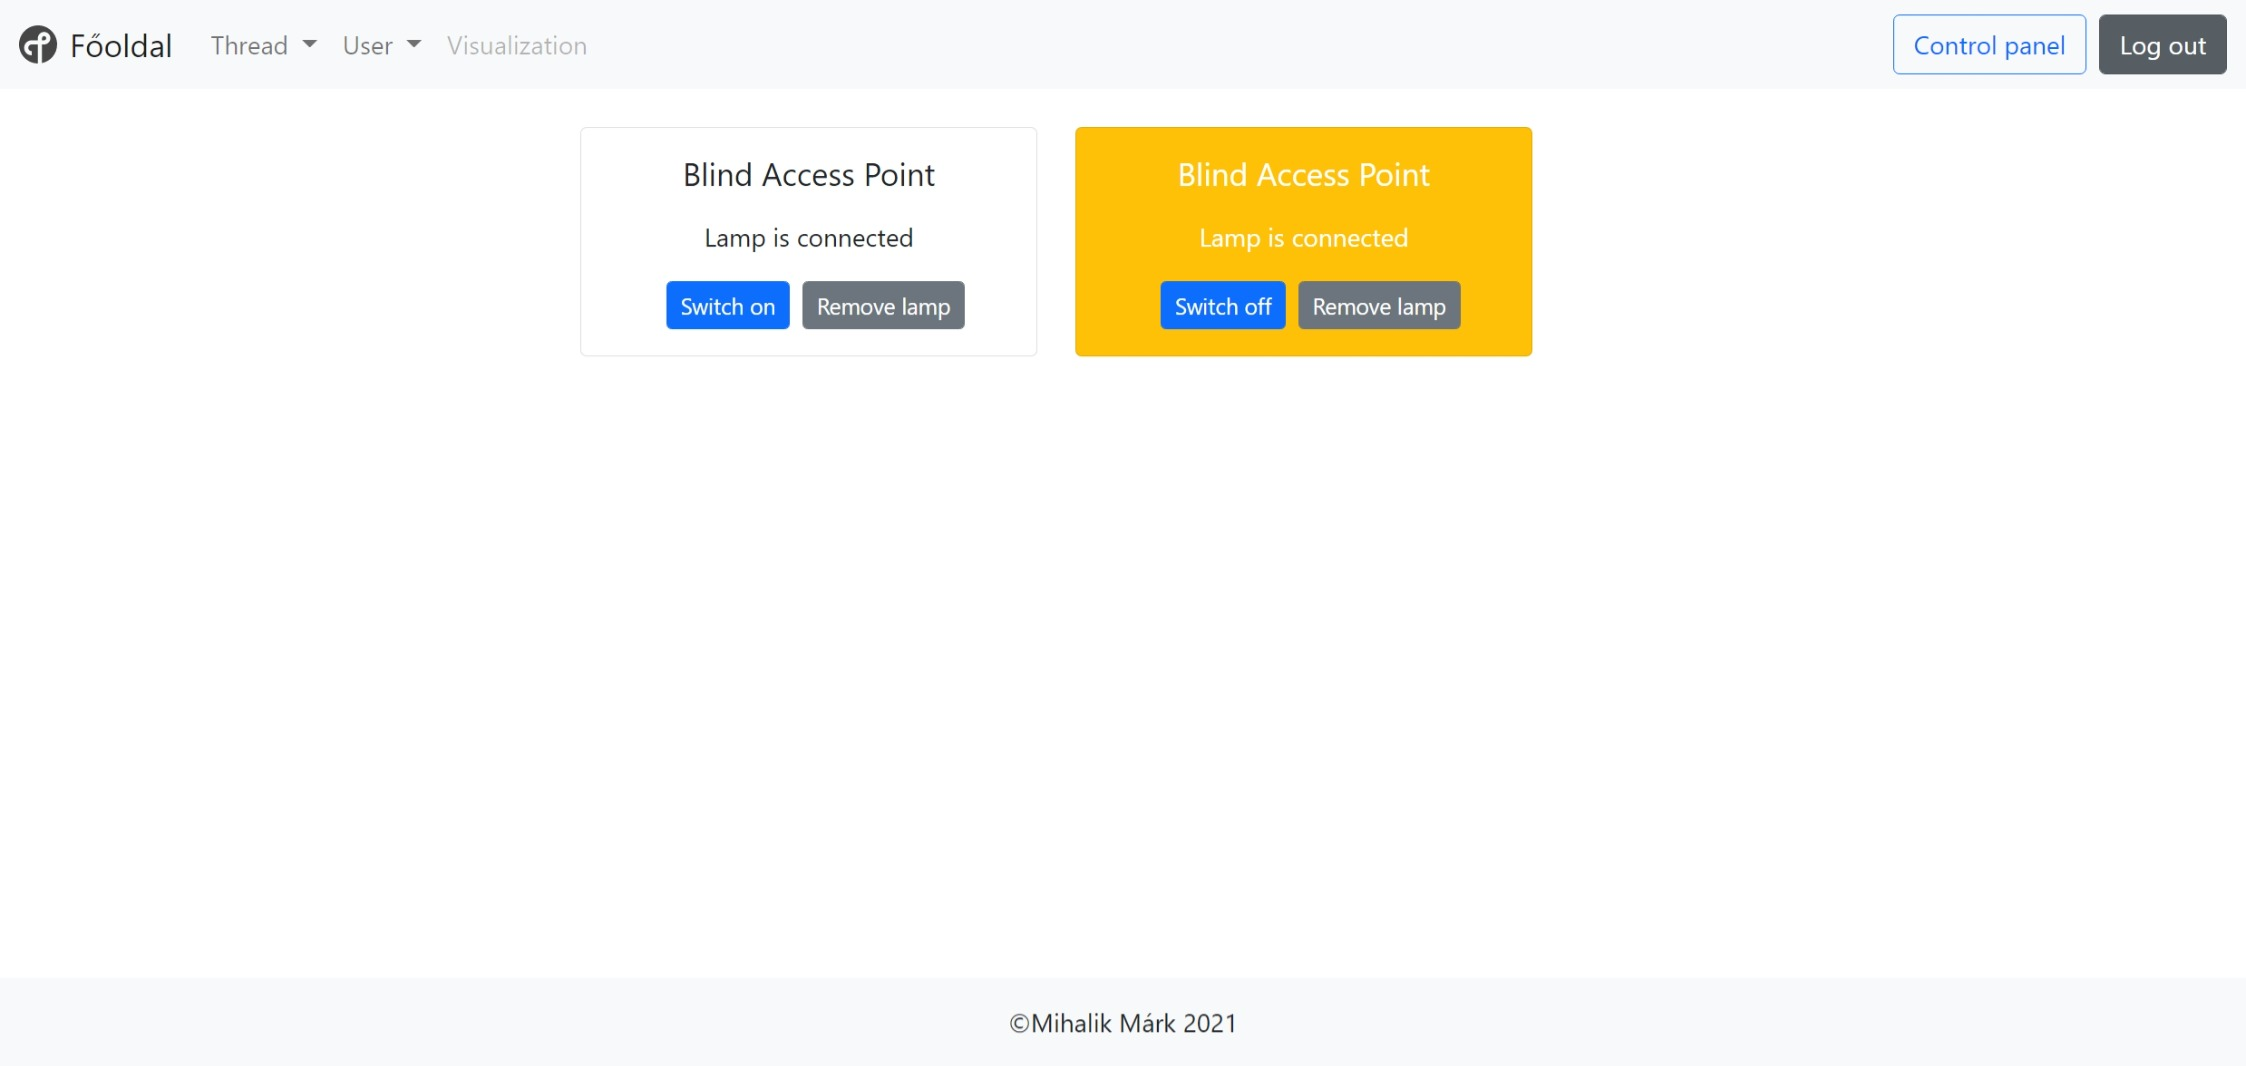
\includegraphics[width=\textwidth]{img/controlpanel.jpeg}
    \caption{The Control Panel}
    \label{fig:controlpanel}
\end{figure}


\subsection{Commissioning}
In this case, to connect a device, a Commissioner is needed on the network. Each connection requires the device's eui64 ID and the device's own password, which is called \textit{Joiner Credential}, which is provided by the programmer in the software created for the device. In my case, this is the Border Router running OpenThread's Commissioner.
Three types of connectivity are thus provided
\begin{itemize}
    \item CLI - Command Line Interface (Linux, MacOS),
    \item Google Commissioner App (Android),
    \item Thread Group Commissioner (Android).
\end{itemize}
The CLI (Command Line Interface) is useful, if the developer wants to test the Thread network and has the eui64 ID and password with a terminal access. Another possible solution is to use the chip's multiprotocol feature, so more protocols can run on the same core, for example a Bluetooth LE and Thread. The second option is a basic Android app by Google that allows QR code connectivity. First, the developer needs an Android smartphone, which is connected to the same home network as the Border Router. Once it appears and the password, that has been created before the network creation is entered. Border Router creates the network itself so according to my Thread network design the manufacturer need to supply this password. The device can join after the QR code reading process is successful. The QR code must contain the eui64 and the joiner password.
\newline
Not much different from this solution is the application published and developed by the Thread Group, which has a much nicer design. Since this is the official app, I use it to connect.
The QR code is generated using the following format:
\begin{center}
    v=1\&\&eui=f4ce36f38f1c9836\&\&cc=BBBBBBBB    
\end{center}
I would like to comment this text, which contains three different part. The first is the version number, since the first version of the Thread is available. The second is eui64 and the third is the password. To generate the code, I use a free Open-Source Program called Zint Barcode Studio\cite{zintdownload}. The QR code must be created according to the ISO18004 standard, where UTF-8 must be chosen as the encoding for the text, or else the app will not be able connect the device.
\begin{figure}[!htb]
    \centering
    
\includegraphics[width=5cm]{img/LampNodeUTF8QRCode5x.png}
    \caption{QR code to connect}
    \label{fig:qrcode}
\end{figure}

\subsection{ThreadGroup application}
\begin{figure}[!htb]
    \centering
    \subfigure[Thread Border Routers]{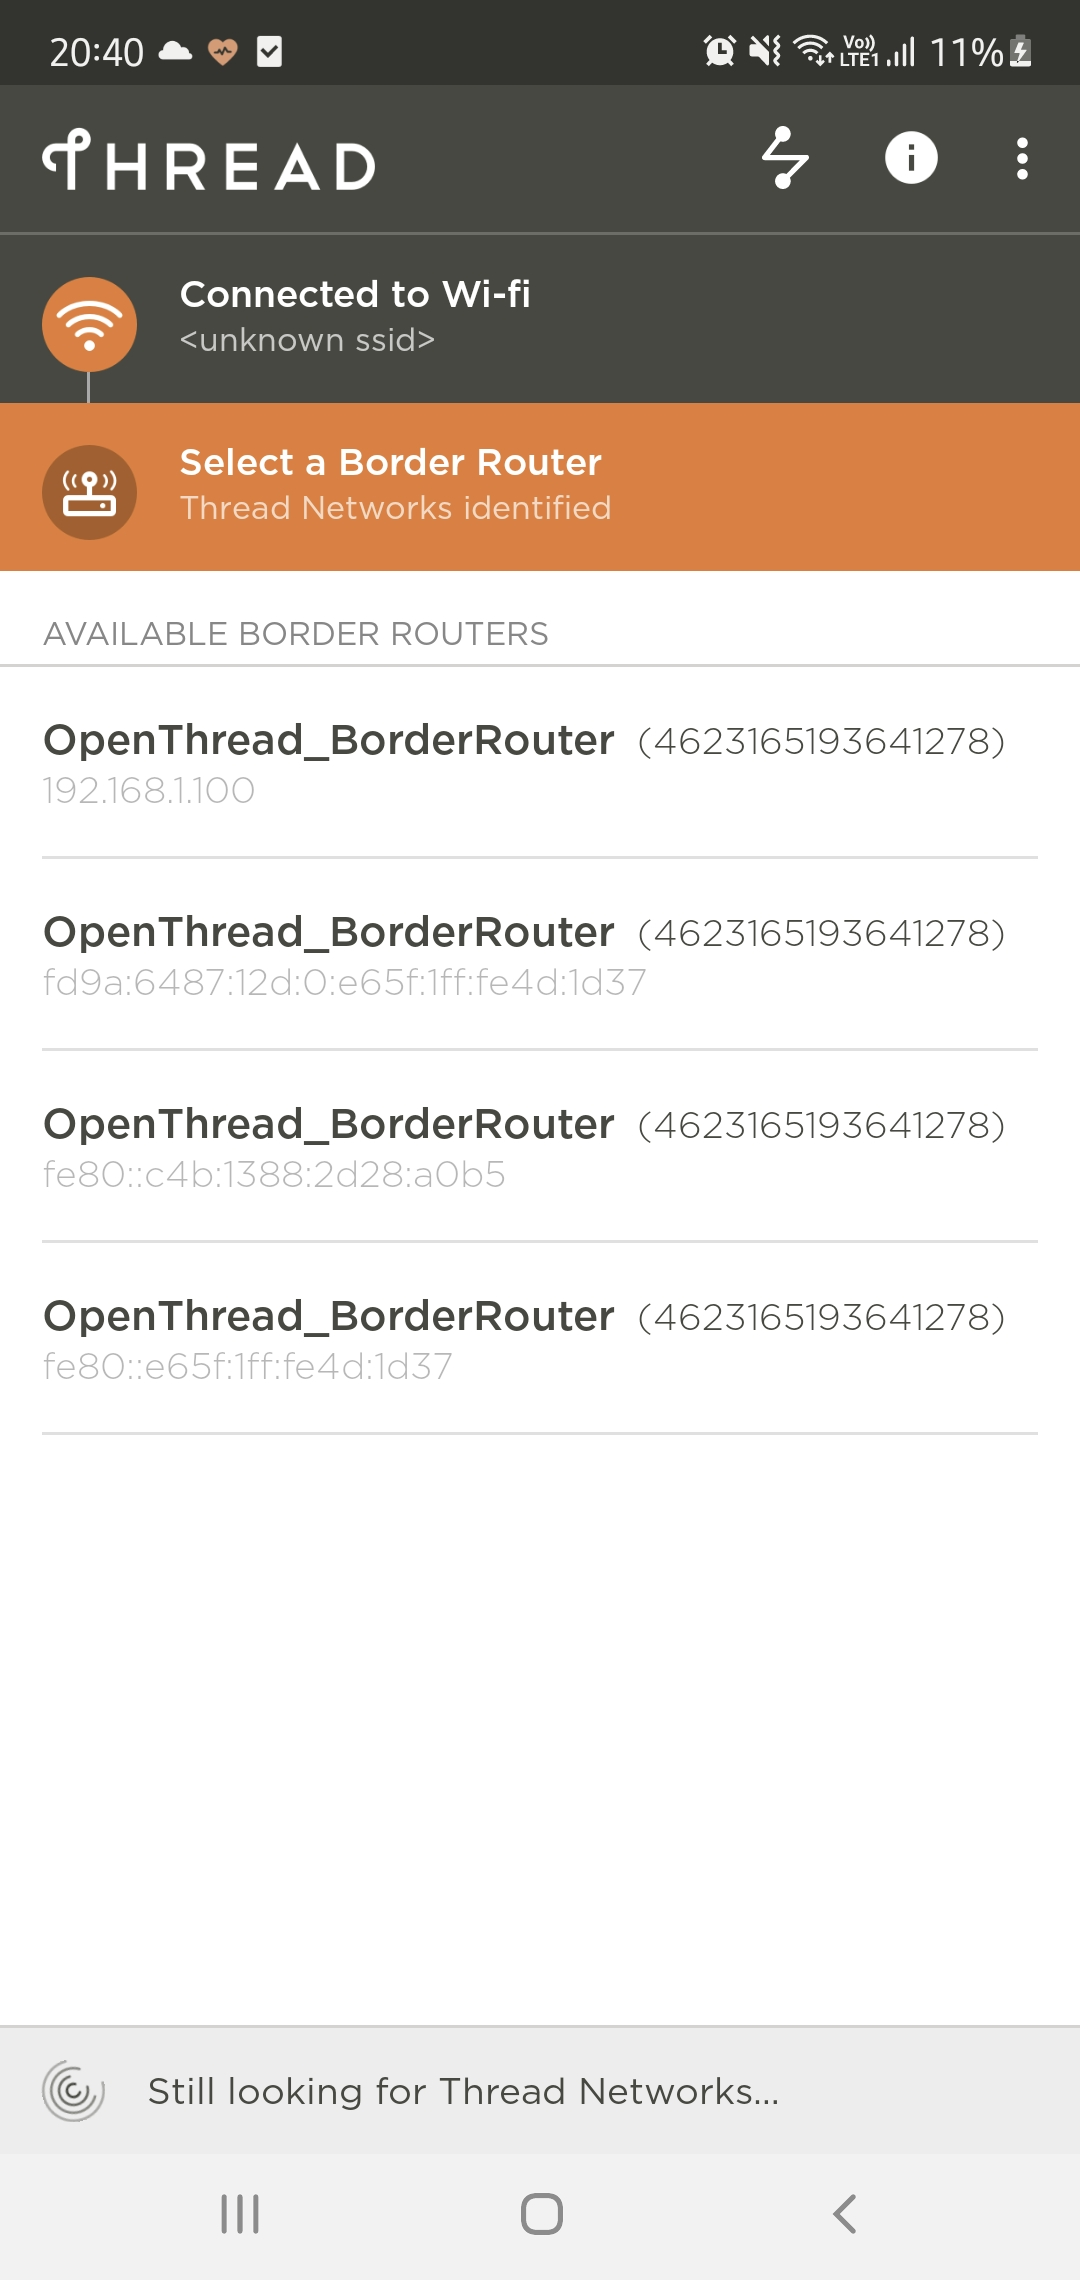
\includegraphics[width=0.3\textwidth]{img/borderouterek.jpg}}
    %\hfill
    \subfigure[Commissioned devices]{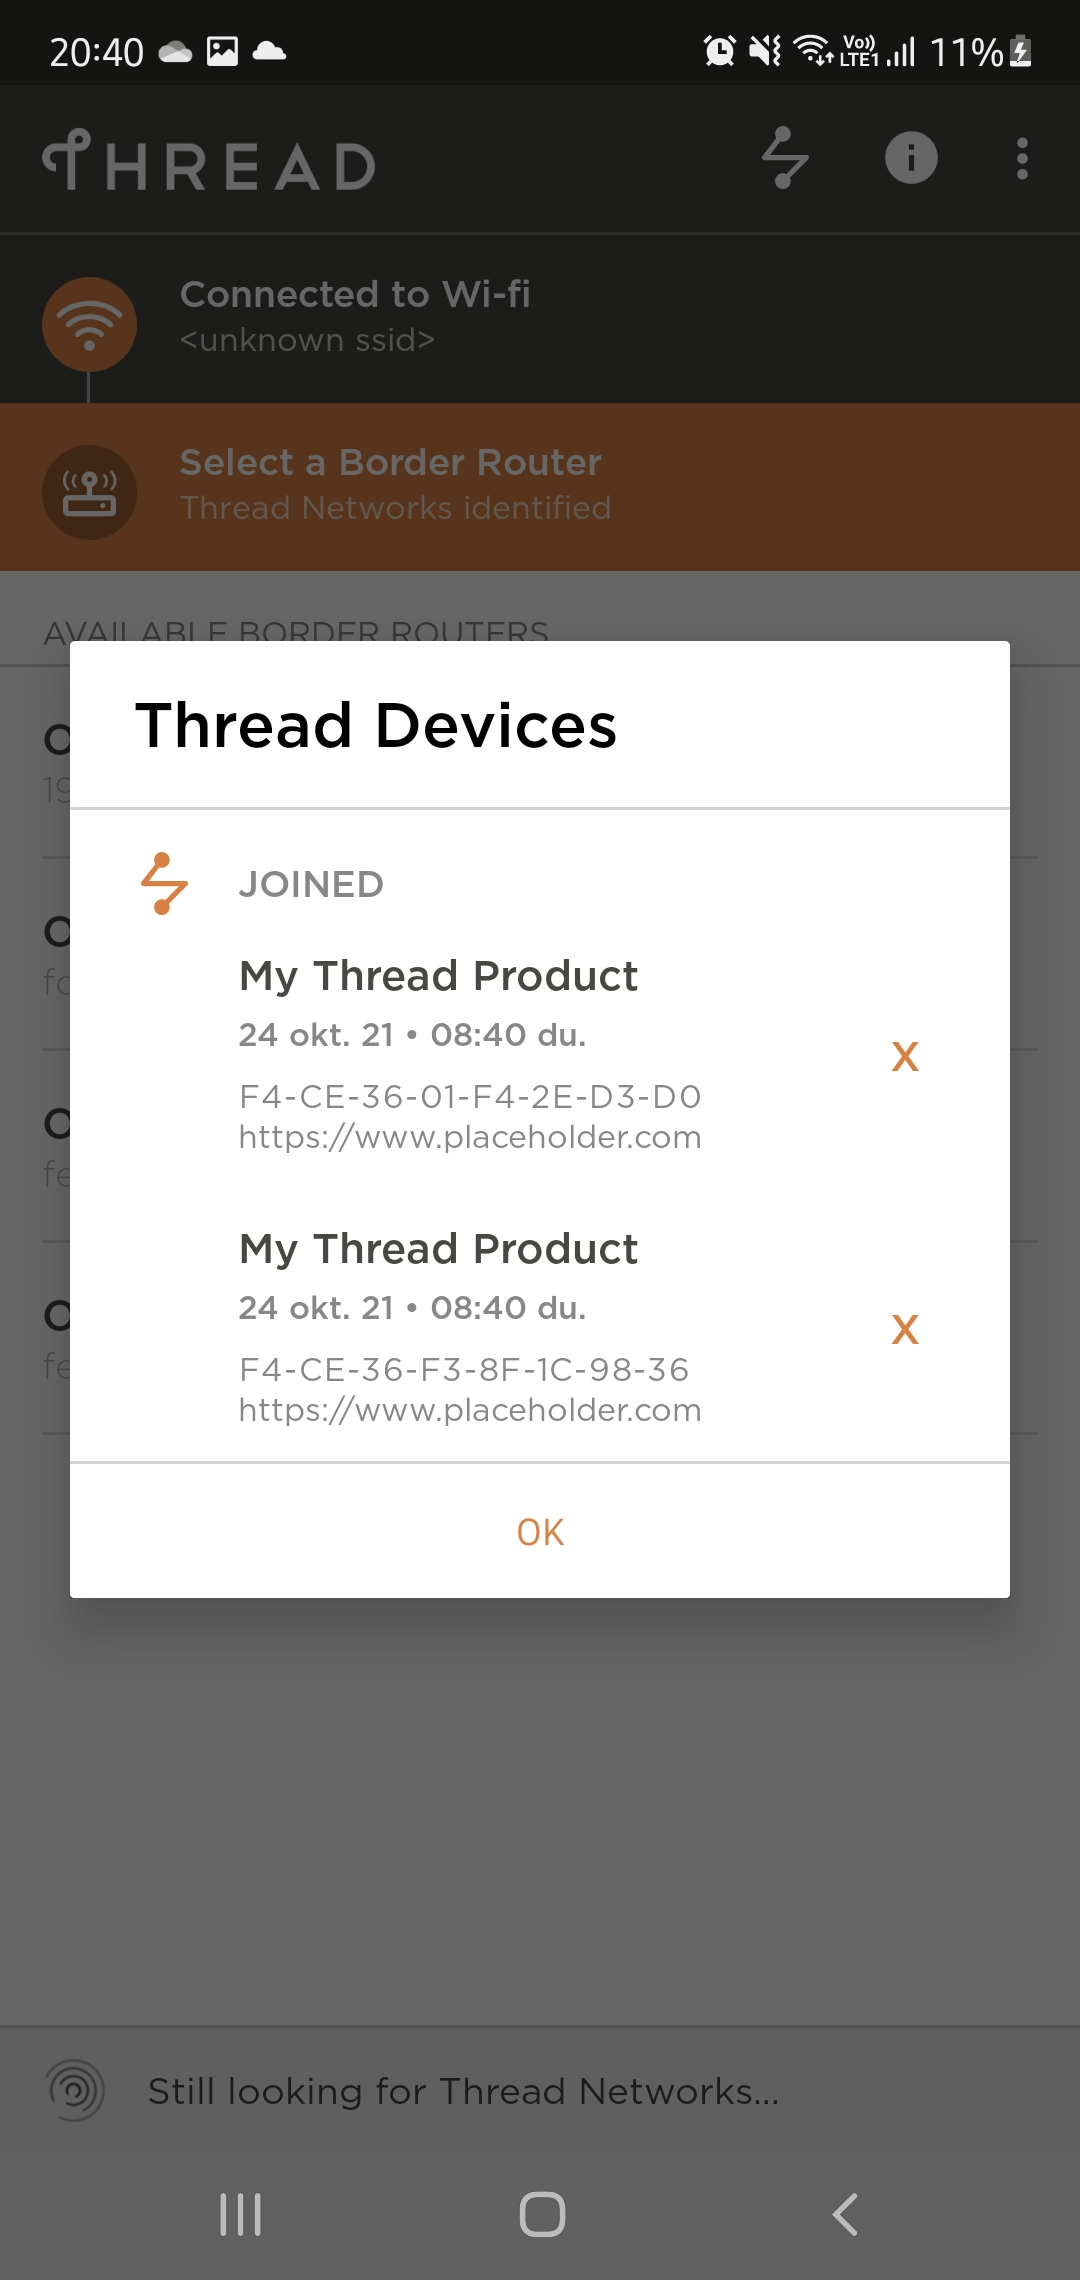
\includegraphics[width=0.3\textwidth]{img/threadeszkozok.jpg}}
    \caption{Thread Group application}
    \label{fig:application}
\end{figure}
Using the app is very simple. As soon as the users are connected to their home network with their Android smartphone, the search for the gateway starts. On the left side of the Figure \ref{fig:application}, can be seen that the one Border Router is available on the home network, which is located at IPv4 address 192.168.1.100. Also, the three other IPv6 addresses below this one belong to the same device. Once one of these is selected, a pop-up window will ask the user to enter the password used to create the Thread network. After the authentication, a QR code scanner will appear on the screen and if the user use it to scan the QR code for the device, which desired to connect, the Commissioner will start. After a few seconds, if the connection is successful, a tick will appear on the display. By clicking on the innermost element of the right navigation bar of the application (a zig-zag line connecting two points) a pop-up window will appear. It is similar to the one shown in the right of Figure \ref{fig:application} with a list of all the devices connected to the Thread network. The user can then remove devices from the network here.

\subsection{Summary of the user interface}
In this section I presented the GUI where the users can be informed the state of their own network and own devices via dynamically changeable cards. I introduced the database model and the Python backend. I also demonstrated a possible solution to the connection process in a Thread network with a smartphone.
\section{Blind Access Point}

\subsection{Introduction}
My goal was to make a universal lamp switcher and door opener that can fit into the 65\,\si{\milli\metre} circular junction box, which is often used by electricians. This device provides a universal solution for Thread routers to increase network coverage while remaining completely hidden from the user's view.


\subsection{Blind Access Point schematic diagram}
\begin{figure}[!htb]
    \centering
    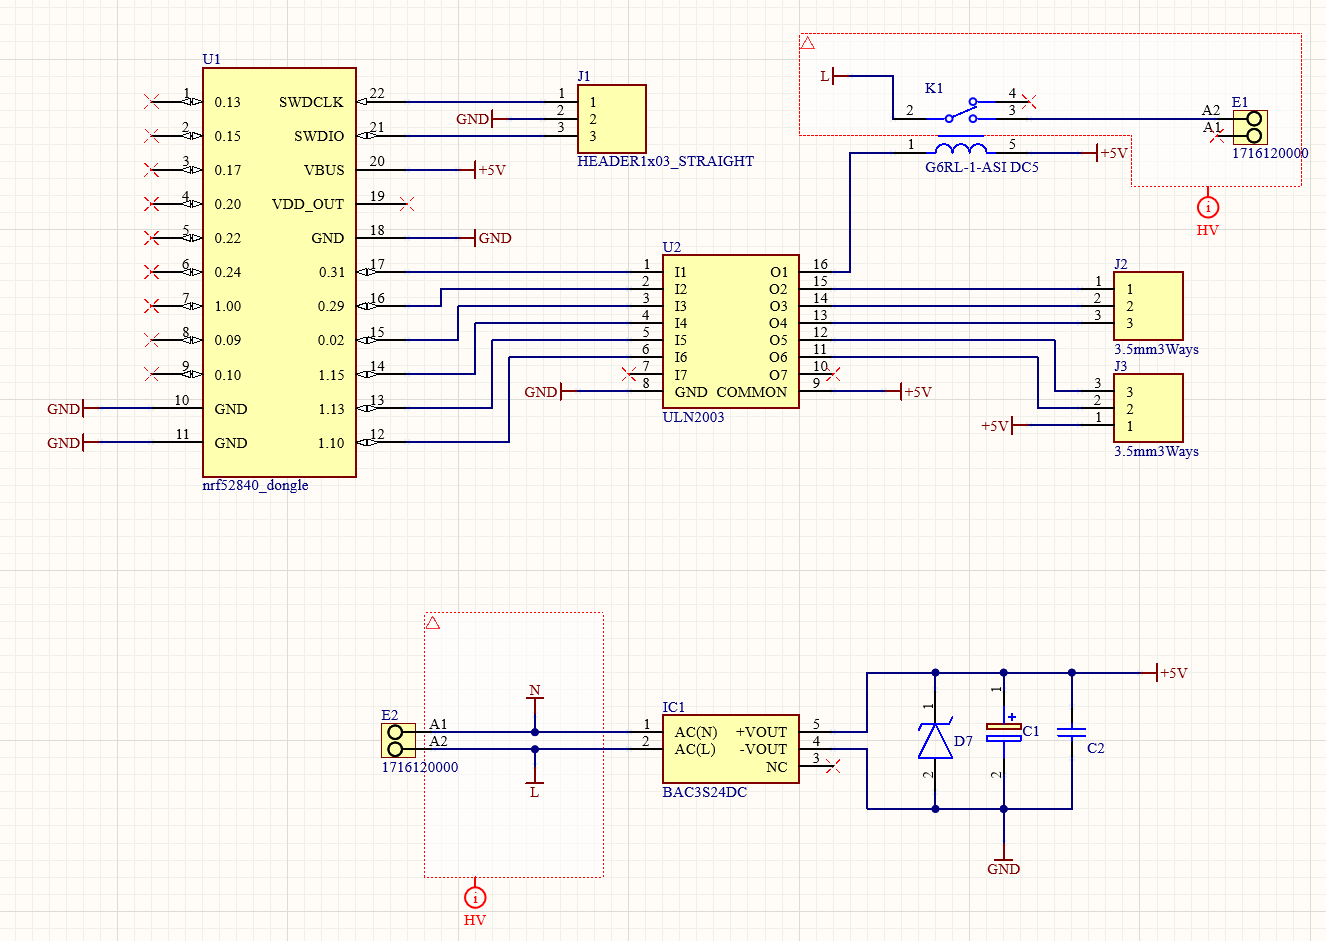
\includegraphics[width=\textwidth]{img/bapschematics.png}
    \caption{Blind Access Point schematic diagram}
    \label{fig:bapschematics}
\end{figure}
\noindent
I equip this device with one of the smallest AC/DC converter power supply (muRata BAC3S05DC) available on the market, which converts 230\,\si{\volt} mains voltage to 5\,\si{\volt} DC. With a 1x1 inch size and a maximum power rating of 3\,\si{\watt}, it is ideal for powering small devices. This module is shown in the lower half of Figure \ref{fig:bapschematics}. To the 5\,\si{\volt} output of the module I design a 7\,\si{\volt} suppressor diode (transient voltage protection), a 220\,\si{\micro\farad} tantalum capacitor (smoothing capacitor) and a 100\,\si{\nano\farad} filter capacitor, but these are also included in the power supply so they are optional.
I solve the switching of the lamp with a 5\,\si{\volt} relay, which connects the phase wire of the module to the lamp. This is important because, if wired correctly, the user's life is not at risk if he accidentally touches the phase point when changing a bulb with the lamp off. The wiring diagram shows the two blocks marked with HV, which is significant as there should be a minimum distance of 1.3\,\si{\milli\metre} between the phase and zero conductor, thus forming an Altium rule.


\subsection{Test panel assembly and software development}
\begin{figure}[!htb]
    \centering
    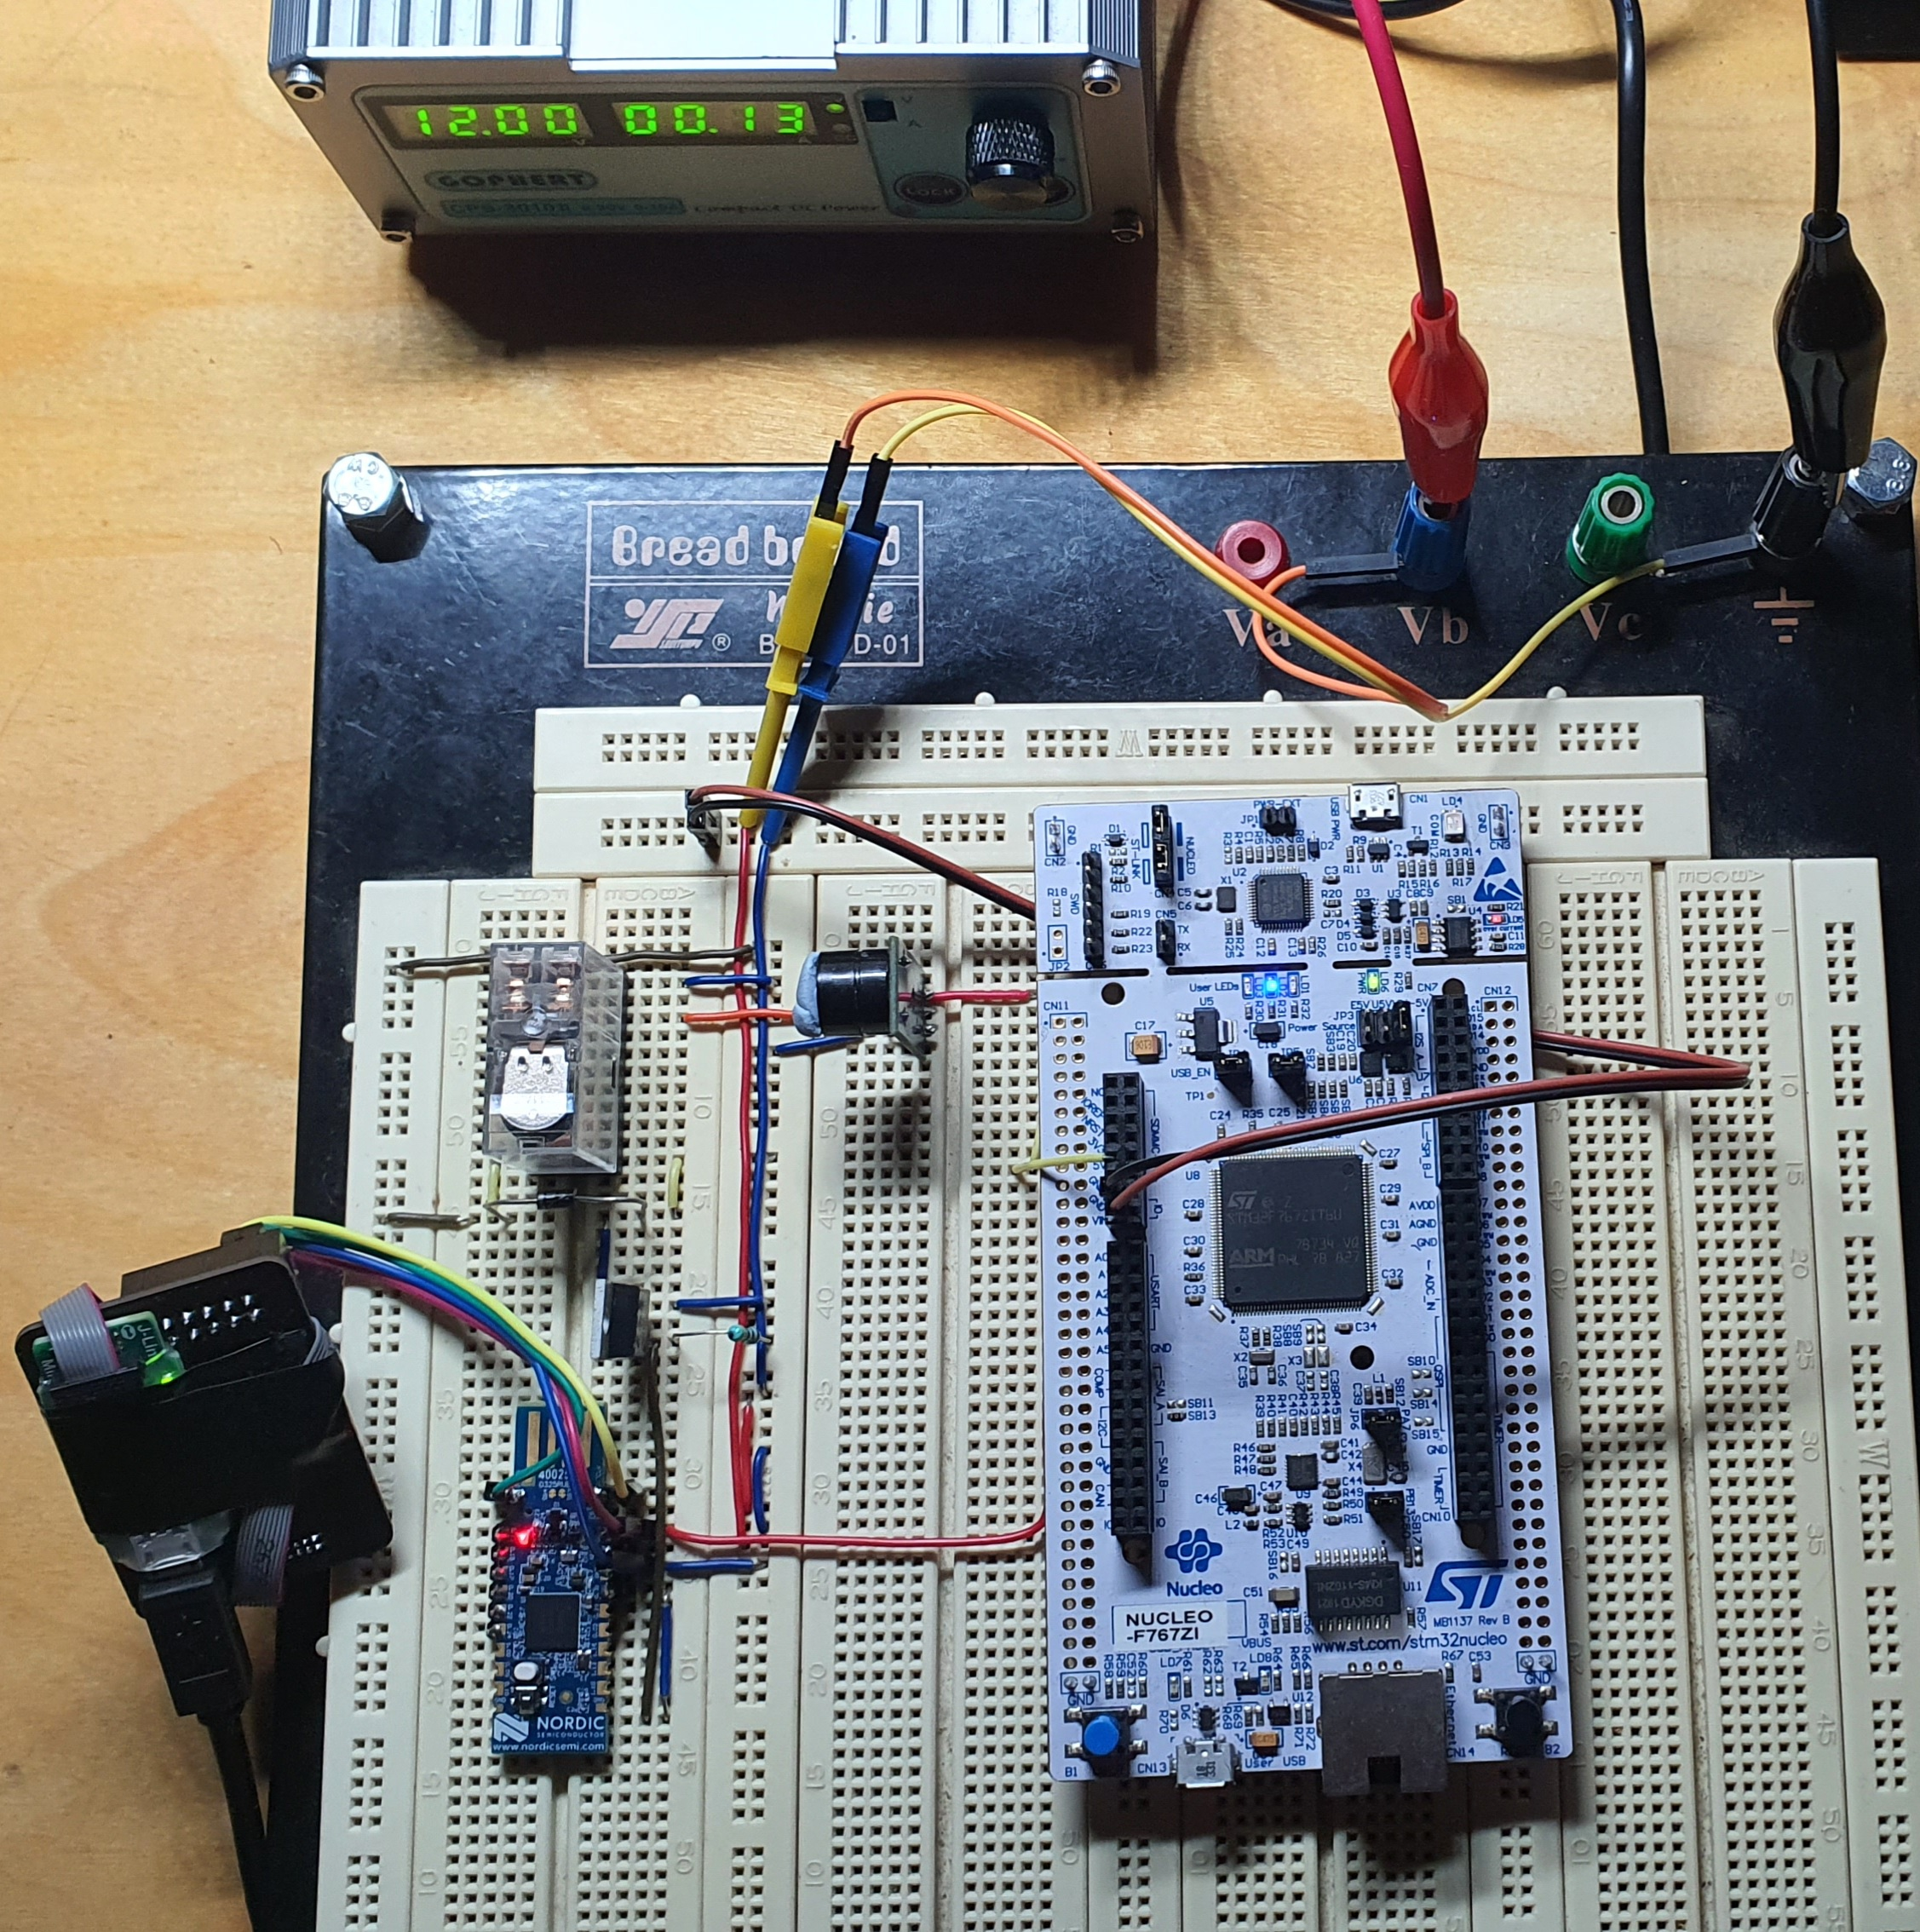
\includegraphics[width=\textwidth]{img/breadboard.jpg}
    \caption{Blind Access Point test panel assembly}
    \label{fig:breadboard}
\end{figure}
\noindent
Before designing the PCB, I created a breadboard concept, which is shown in Figure \ref{fig:breadboard}. I did not have the necessary components for the concept, so I substituted them with my tools at home and made the software accordingly. I wrote the software in the already familiar Zephyr, where two threads perform the device tasks. One thread handles the OpenThread and the Border Router address query, connection initiation and management functions and the special cases, what the programmer needs to handle. One such case is the \textit{callback} function that is called automatically after the device is connected, which gives information about the role of the device in the network. The other thread is responsible for checking the status of the lamp and switching the lamp. I implement this by having the device query the Border Router every half a second, then read the state of the lamp from the comment column of the device table from the database stored on the device, based on the device's eui64 ID if it is connected. In response, it sends a text to the device, which can be either "true" or "false". This is processed by the device and thus influences the state of the lamp.


\subsection{Blind Access Point PCB design}
In the PCB plan (shown in Figure \ref{fig:bap3D}) I tried to place the line voltage as far from the 5\,\si{\volt} line as possible. I designed a cut-out between the phase and zero conductor strips at the 230\,\si{\volt} part, so that I could create a sufficiently large spacing, since in dry air the breakdown voltage is approximately 1.3\,\si{\kilo\volt} per 1\,\si{\milli\metre}. In humid air, it can drop to 600\,\si{\volt}\cite{airbreakdownvoltage}, but this is still almost twice the maximum amplitude of the 230\,\si{\volt} mains voltage. I removed the solder mask from the high voltage section to ensure that solder mask would not absorb moisture, thus reduce the breakdown voltage.
In case one lamp is not enough, five outputs of 5\,\si{\volt} are available for a relay module. The control of the relays is solved by an IC (ULN2003) with six independent Darlington switches, which has flyback diodes on each output, thus ensuring a longer lifetime.

\begin{figure}[!htb]
    \centering
    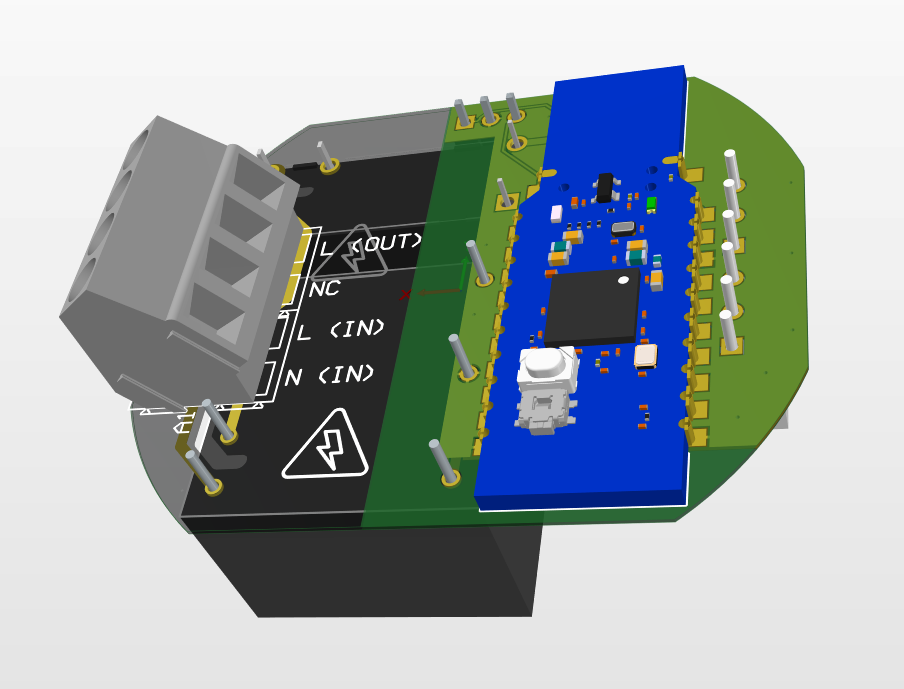
\includegraphics[width=\textwidth]{img/bap3d.png}
    \caption{Blind Access Point in 3D viewer}
    \label{fig:bap3D}
\end{figure}


\section{Minimal Sensor Node}

\subsection{Introduction}
As a third device, I created a circuit that can collect environmental data with minimal energy consumption. These include brightness, temperature, humidity and depending on the sensor, a barometric pressure sensing function. A further consideration was to be lightweight and small so that it could be placed or attached anywhere to collect data.

\subsection{Minimal Sensor Node schematic diagram}
\begin{figure}[!htb]
    \centering
    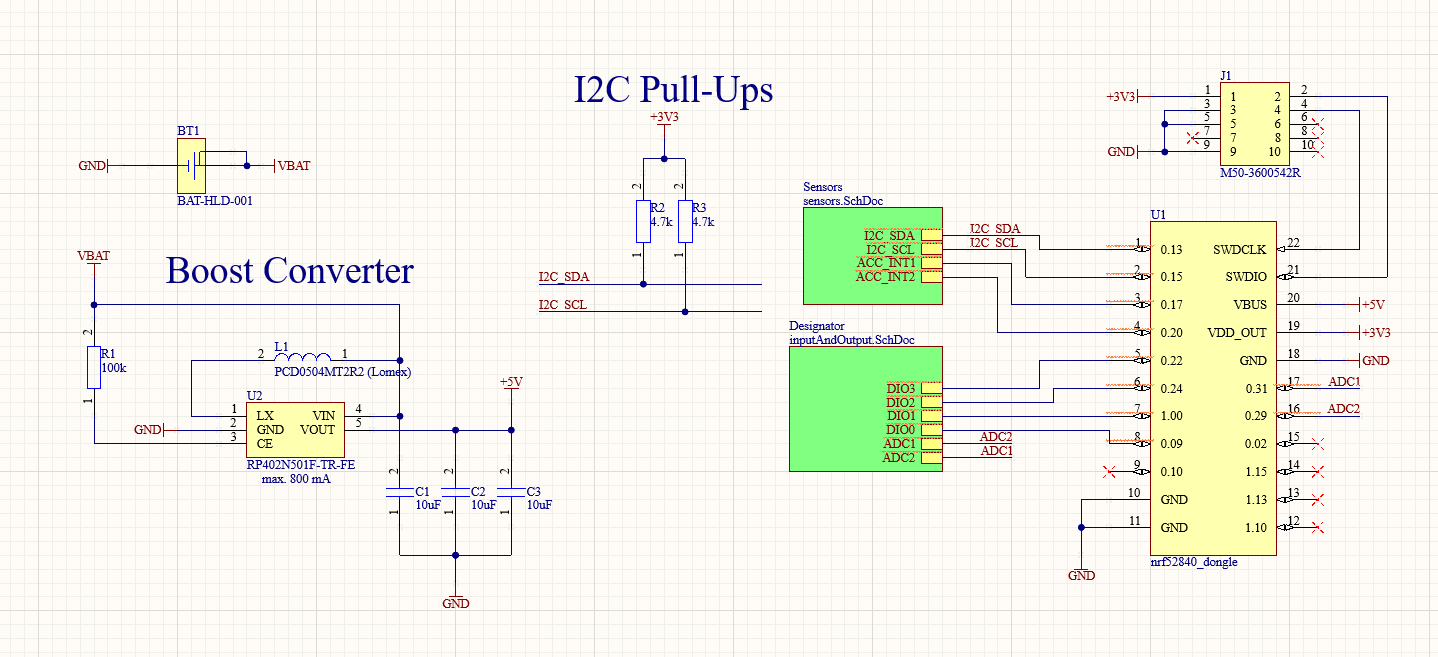
\includegraphics[width=\textwidth]{img/minimalsensornodeschematics.png}
    \caption{Minimal Sensor Node schematic}
    \label{fig:minimalsensornodeschematic}
\end{figure}

\begin{figure}[!htb]
    \centering
    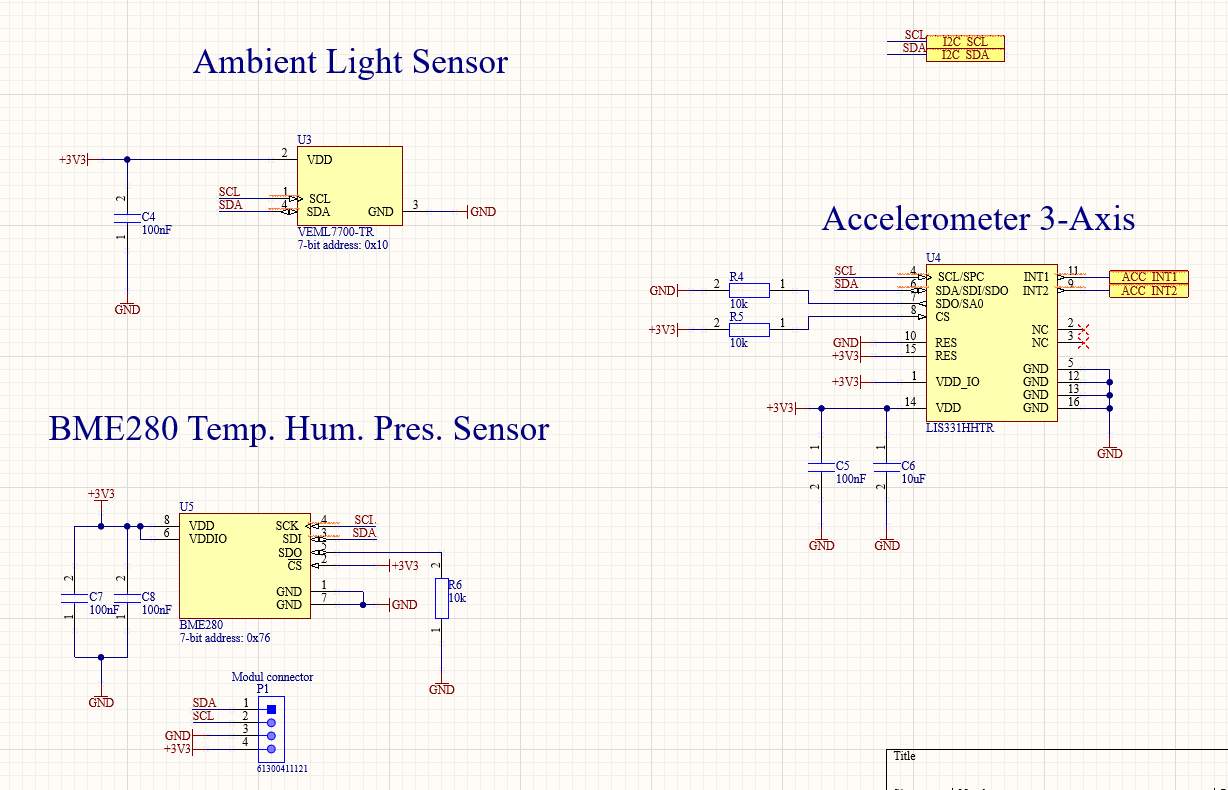
\includegraphics[width=\textwidth]{img/minimalsensornodeschematicssensors.png}
    \caption{Minimal Sensor Node schematic}
    \label{fig:minimalsensornodeschematicssensor}
\end{figure}
\noindent
Figure \ref{fig:minimalsensornodeschematic} shows the schematic of the Minimal Sensor Node. On the left side of the picture is a button coin cell battery holder, into which a CR2032 type 3V Lithium battery can be inserted. The dongle is designed for 5V power supply, so to avoid non-factory modifications to these modules, I saw fit to use a 5V boost converter using an IC with serial number RP402. This IC requires few elements (a couple of capacitors and an inductor) and has high efficiency. The right side of Figure \ref{fig:minimalsensornodeschematic} shows the nrf52840 dongle itself, connected to the outputs, inputs and sensors. Figure \ref{fig:minimalsensornodeschematicssensor} shows the sensor part of this node. I design 3 sensors for this device, one is a BME280 temperature, humidity and barometric pressure sensor, another is a VEML7700 light sensor and the third is a LIS331 3-axis accelerometer sensor.

\subsection{Minimal Sensor Node PCB design}
\begin{figure}[!htb]
    \centering
    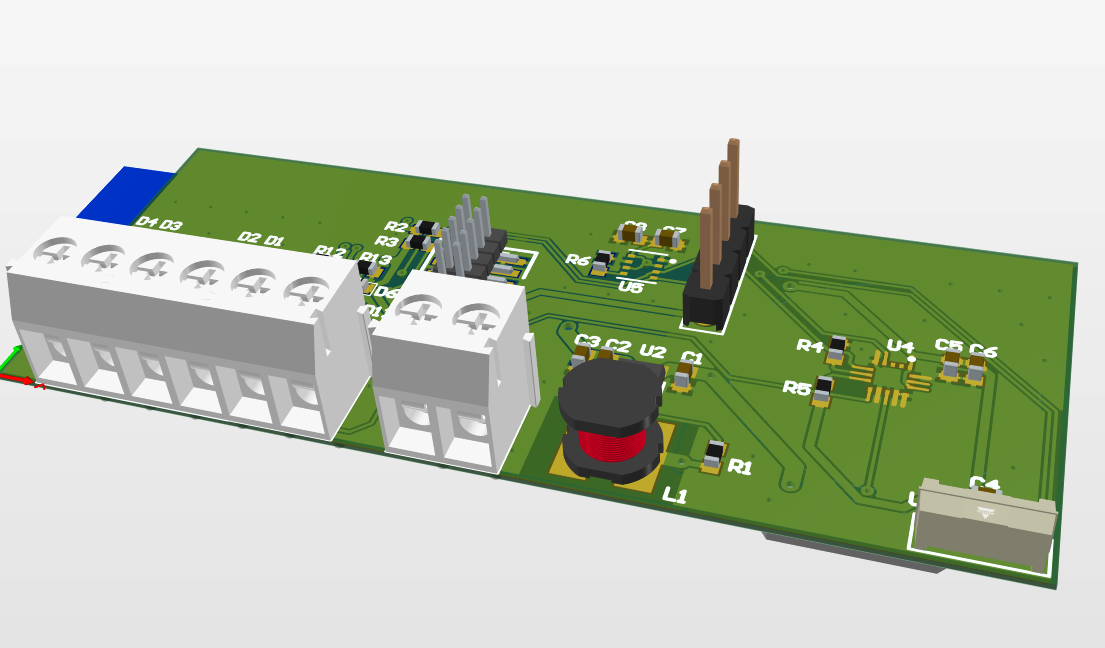
\includegraphics[width=\textwidth]{img/minimalsensornodepcb3dupper.png}
    \caption{Minimal Sensor Node - Upper side of PCB}
    \label{fig:powernodepcbup}
\end{figure}
\noindent
The PCB plan shows the top side where the sensors are located. The BME280 sensor is an LGA package, so I use a breakout board for it instead, which already has the pull-up resistors and filter capacitors for the unused pins of the chip. On the right side is the accelerometer and the VEML7700 light meter. In the Figure \ref{fig:powernodepcbup} the down side of this PCB is not shown, but there is the dongle module and the coin-cell battery holder.

\subsection{Webpage}
\begin{figure}[!htb]
    \centering
    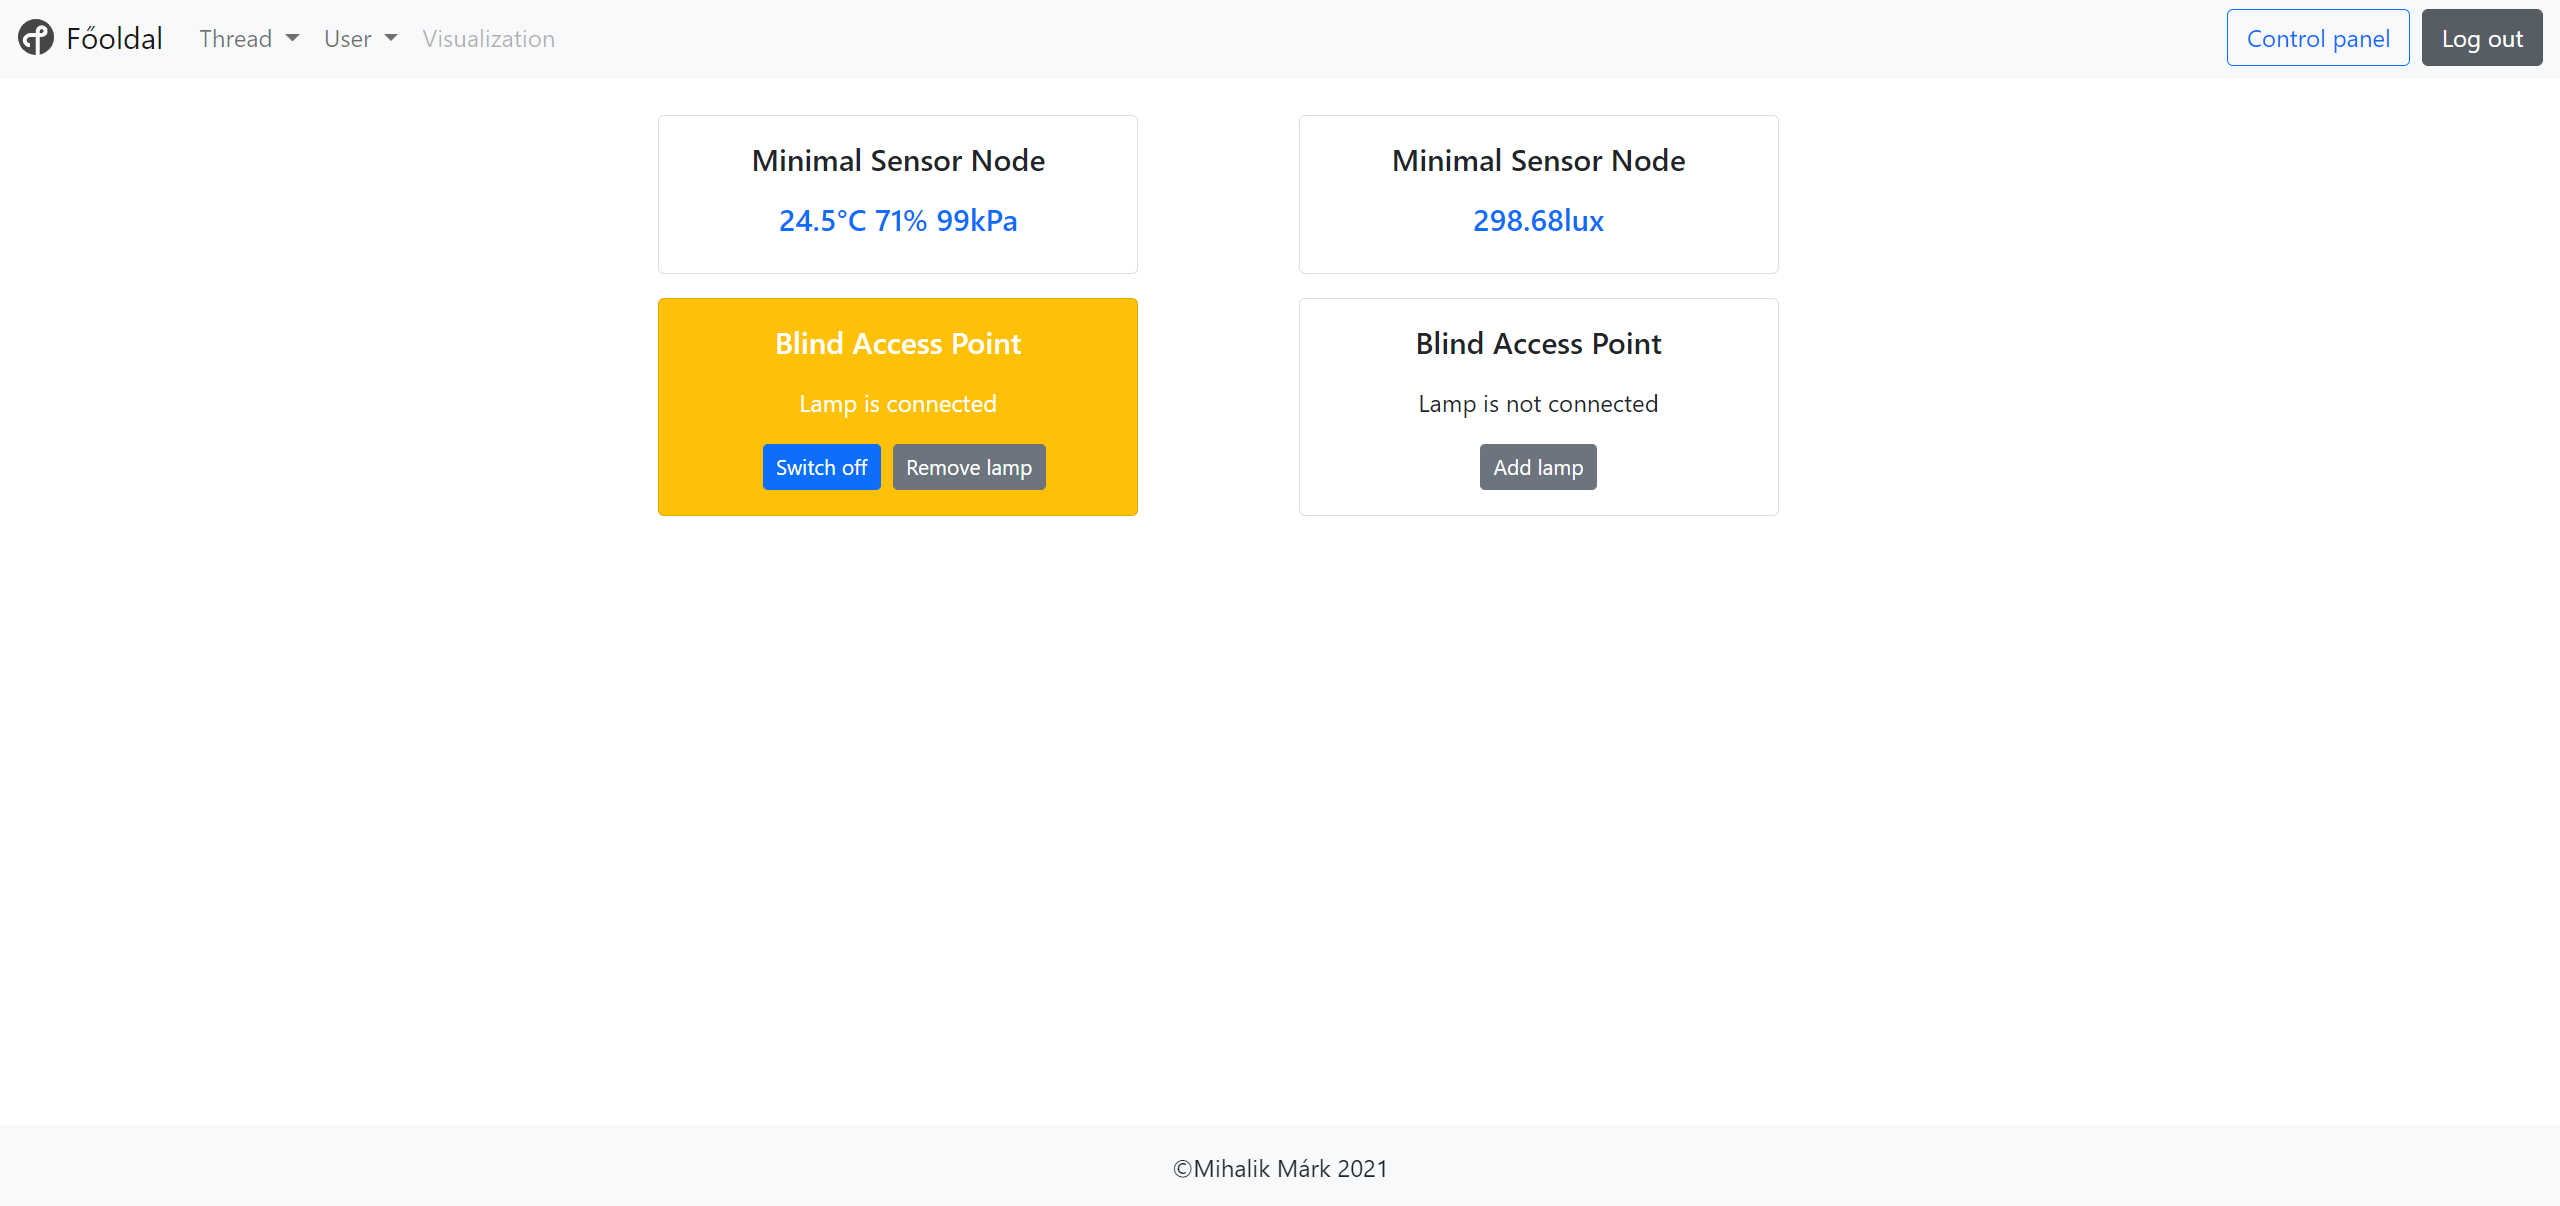
\includegraphics[width=\textwidth]{img/minimalsensornodeWebpage.png}
    \caption{Power Node PCB}
    \label{fig:powernodewebpage}
\end{figure}
\noindent
On the webpage there is the \textit{Minimal Sensor Node} on two different cards. In this moment this node can be used only with the BME280 or with the VEML7700. This is because Zephyr requires a specific driver, because its drivers split into parent and child. For example the parent is the I2C\_0 peripheral and the child consists of the sensors on the bus. I made the VEML7700 driver with the I2C\_0 peripheral, so I am not able to use the Zephyr BME280 driver, as I can not use the parent and child drivers together.


\section{Power Node}
\subsection{Introduction}
My goal was to design an MTD device that could be powered by a larger capacity Lithium-Polymer battery cell and integrate on one circuit five different target devices, which could be
\begin{itemize}
    \item PIR (Pyroelectric Infrared Sensor) node, i.e. a motion detection node,
    \item a motor driver with a higher power output 5\,\si{\volt} (e.g. a low power irrigation pump),
    \item an environmental monitoring node (temperature, humidity, air pressure and brightness),
    \item node for connecting higher power devices with external power requirements,
    \item motion sensor, door opening sensor node. 
\end{itemize}
All of these are available on a PCB and depending on the end use, one or more functions are available depending on the soldering of the different parts.


\subsection{Power Node schematic}
\begin{figure}[!htb]
    \centering
    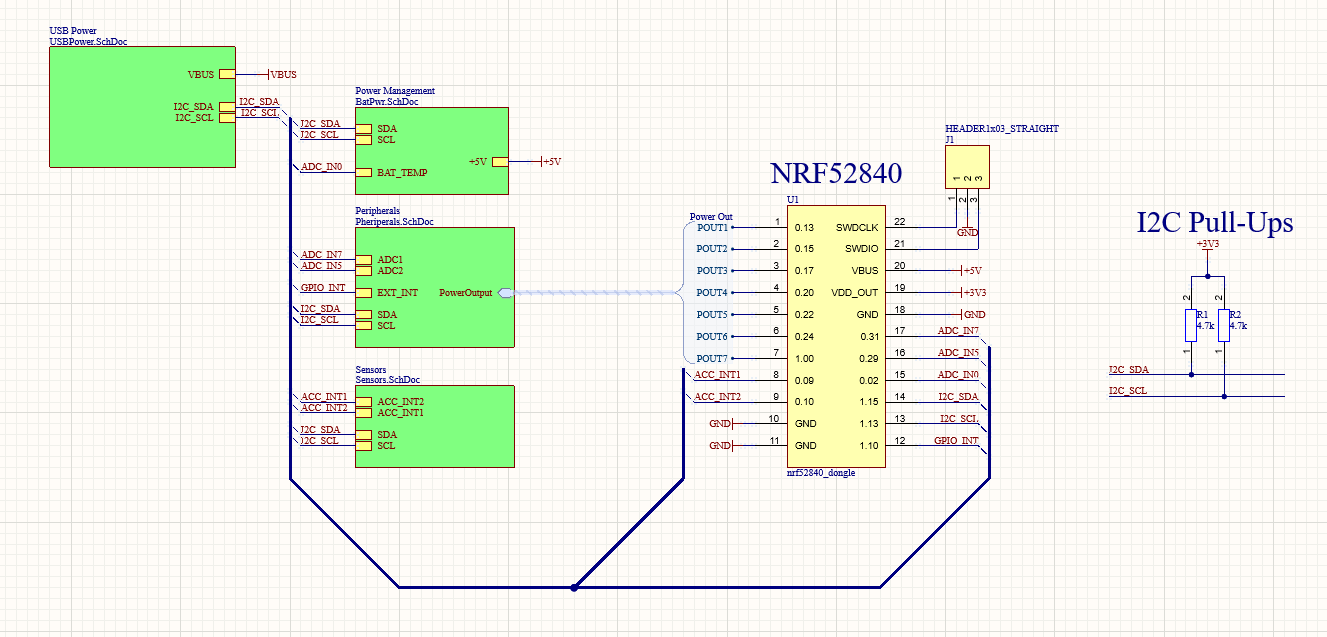
\includegraphics[width=\textwidth]{img/powernode.png}
    \caption{Power Node schematic}
    \label{fig:powernodeschematics}
\end{figure}
\noindent
Figure \ref{fig:powernodeschematics} shows the schematic of this device. From top left down, the first box indicates the USB Type-C charging connector, which allows the device to be operated from an external 5\,\si{\volt} power supply. The I2C bus is used to read the power meter IC. To the right of this block is the charger and the \textit{Battery Protection} (short \textbf{BPS}) circuit to protect the Li-Po battery. The I2C bus is used to access the measured data of another power meter IC, as this is used to provide the microcontroller with information about the status of the voltage source, which can later be used to signal the user when the device needs charging. On the other hand, it is a way to protect against the user drawing too much current from the system, which would lead to the device's failure. This block also contains a 5\,\si{\volt} boost (step-up) converter, which converts the source voltage from 3 to 4.2\,\si{\volt} at 80-90\,\% efficiency. The peripherals section contains three outputs with a load capacity of 200\,\si{\milli\ampere} (protected by 200\,\si{\milli\ampere} polyfuses) and two pulse relays for switching external power up to 48\,\si{\volt}. I extend the digital inputs and outputs with a GPIO expander (GPIO-Expander), as there are not enough inputs and outputs available on the Dongle. Furthermore, they operate at a logic level of 5\,\si{\volt}, because the IC (TCA6408) I use. It requires a separate power supply for the microcontroller communication and the GPIOs, so it also functions as a level shifter. In the event of a change in input, an interrupt is generated to the microcontroller. There are two analog inputs connected to the wired pins of the nRF52840 ADC with overvoltage protection. In the sensor section, there is a VEML7700 I2C light sensor, a BME280 temperature, humidity and barometric pressure sensor (both IC and module on the panel due to the LGA encapsulation) and an accelerometer sensor.

\subsubsection{Power Node PCB}
\begin{figure}[!htb]
    \centering
    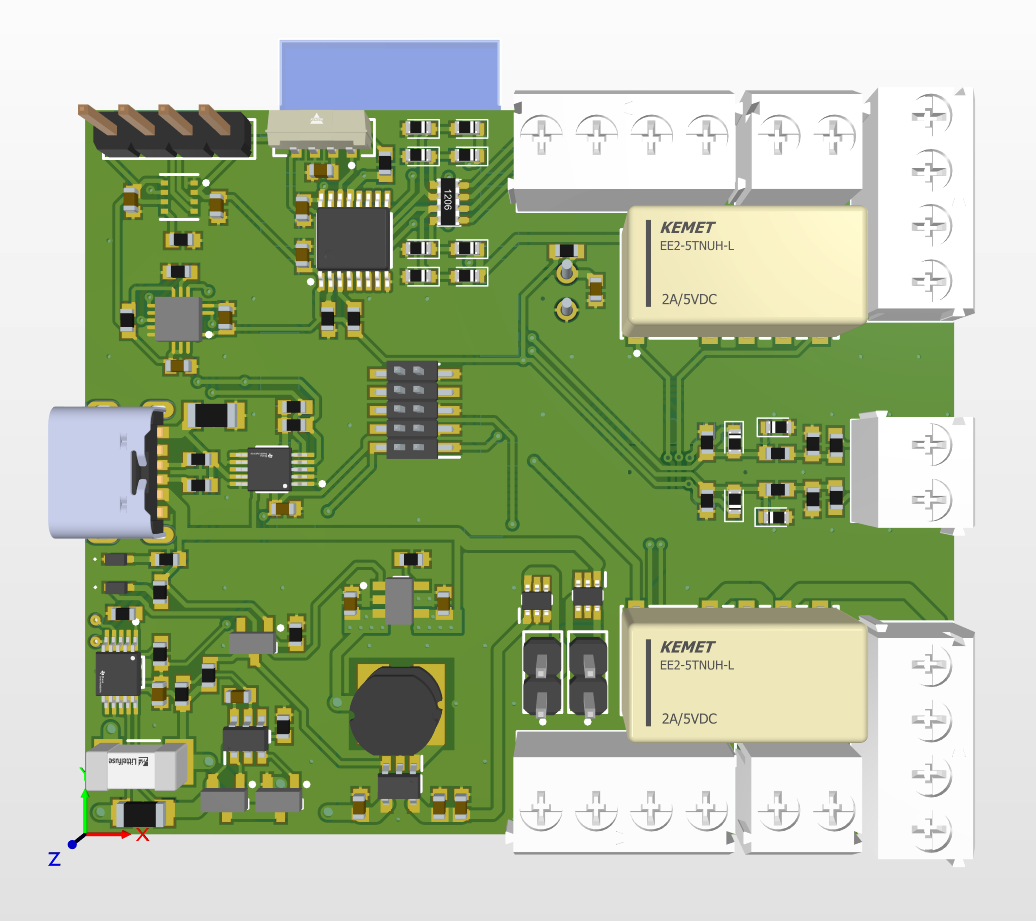
\includegraphics[width=\textwidth]{img/powerboardpcbkesz.png}
    \caption{Power Node PCB}
    \label{fig:powernodepcb}
\end{figure}
At the moment, the PCB plan is half-finished, as only the components have been installed on the 3D design so far. The panel size is going to be 50x60\,\si{\milli\metre\squared} as the chose Li-Po cell dimensions comply with it. The layout is shown in Figure \ref{fig:powernodepcb}. This plan is not realised as many of the necessary parts could not be ordered due shortages in the supply chain.
\clearpage
\section{Implemented Thread network}

\subsection{Thread network topology}
With the three Blind Access Points and the Border Router I have created a test of my own Thread network. I did this in an apartment with a floor space of 40\,\si{\metre\squared} and placed the four devices on four points in the house. After successfully connecting each device, the resulting topology was as shown in Figure \ref{fig:topology}. It can be clearly seen that three of the four devices were in the Router role and one was in the End Device (Child) role. This is observed because OpenThread tries to keep the number of routers participating in the whole Thread network between 16 and 23 devices. This topology has evolved because, at the time the image was taken, one of the FTD devices had not yet been able to designate itself as a router. During testing, the devices were in stable connection with each other and all devices were available in the network.
\begin{figure}[!htb]
    \centering
    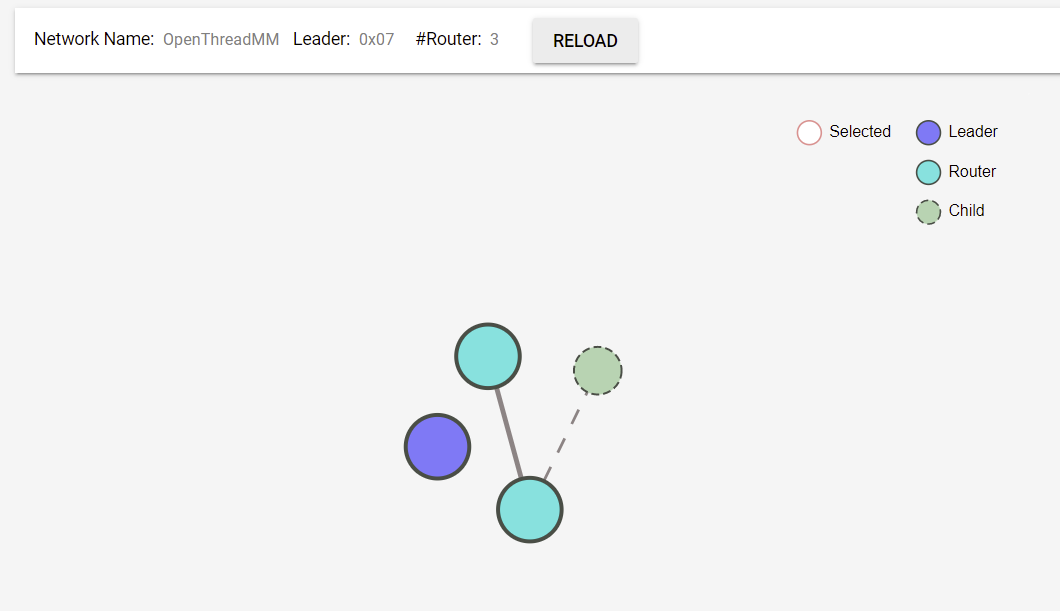
\includegraphics[width=\textwidth]{img/topologia.png}
    \caption{My Thread network topology}
    \label{fig:topology}
\end{figure}

\pagebreak
\subsection{Border Router in operation}
\begin{figure}[!htb]
    \centering
    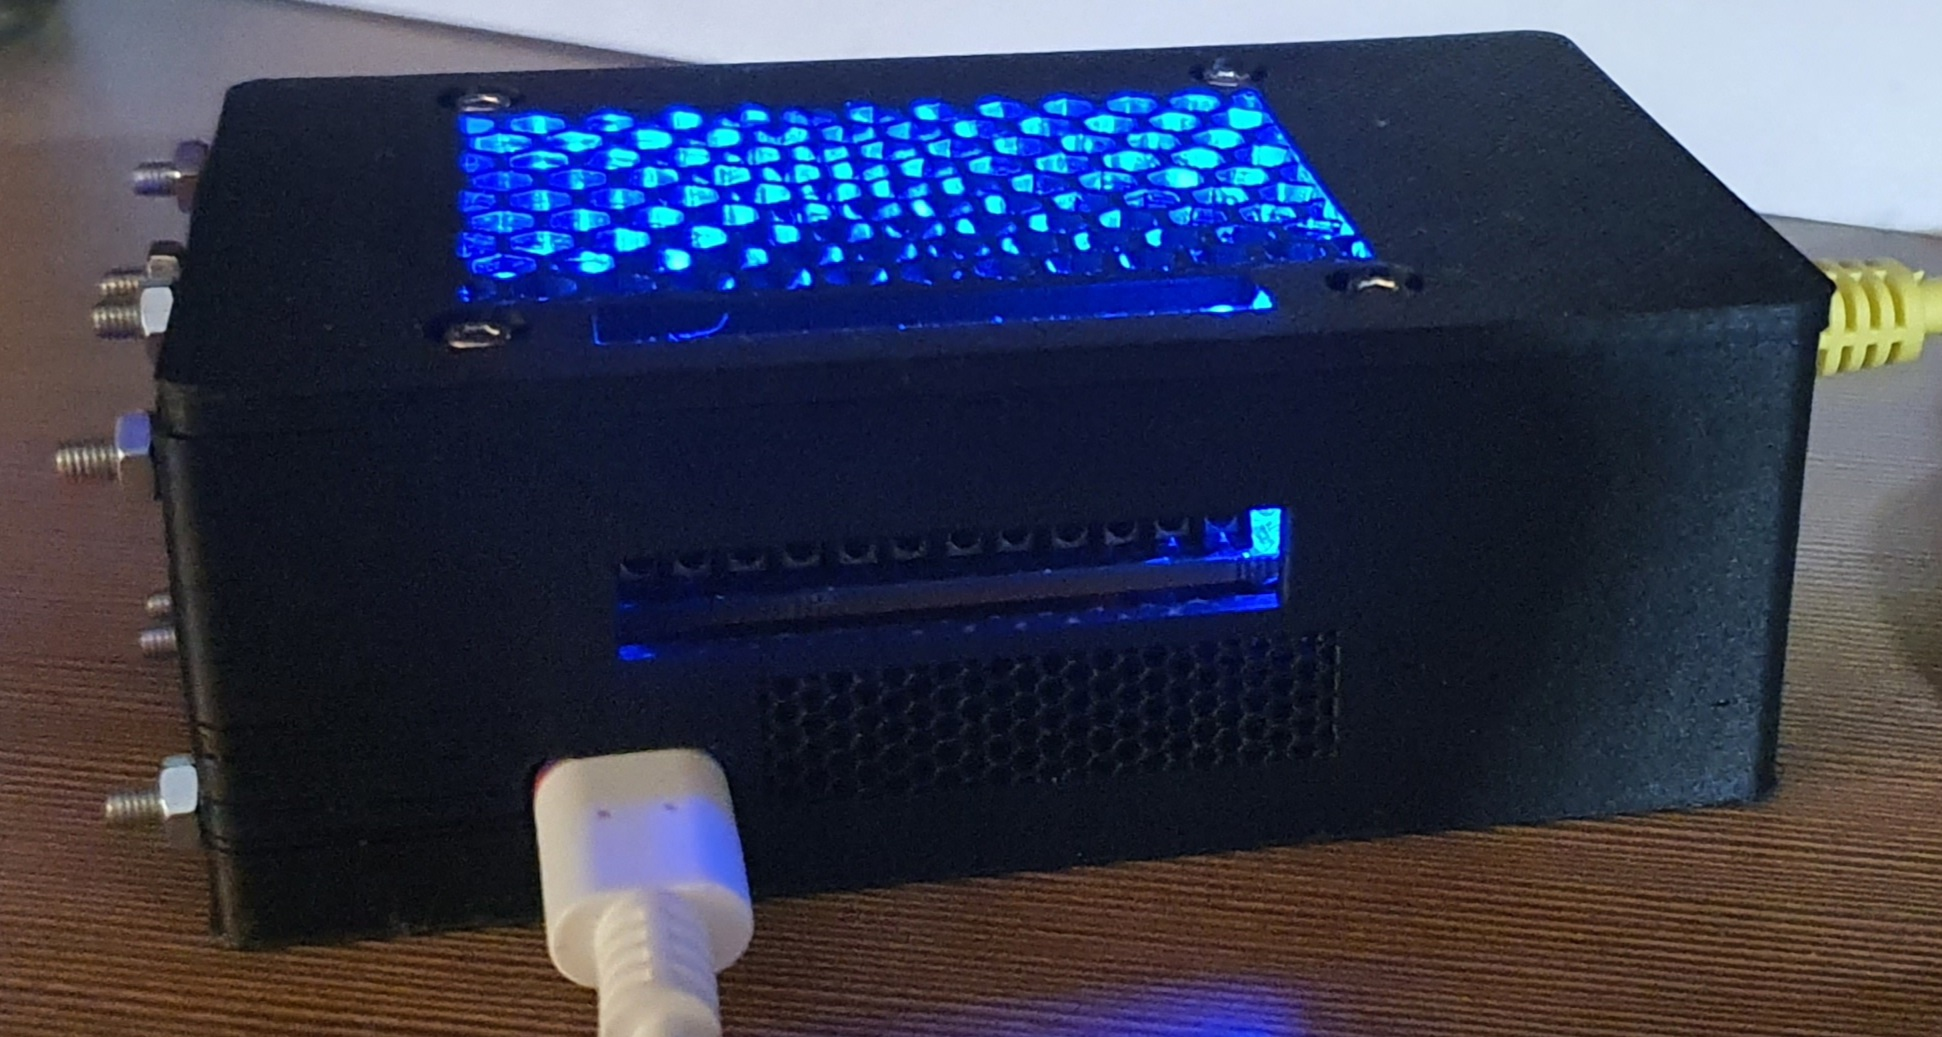
\includegraphics[width=\textwidth]{img/valosborderrouter.jpg}
    \caption{Assembled Border Router}
    \label{fig:realborderrouter}
\end{figure}

\subsection{The completed Blind Access Point}
\begin{figure}[!htb]
    \centering
    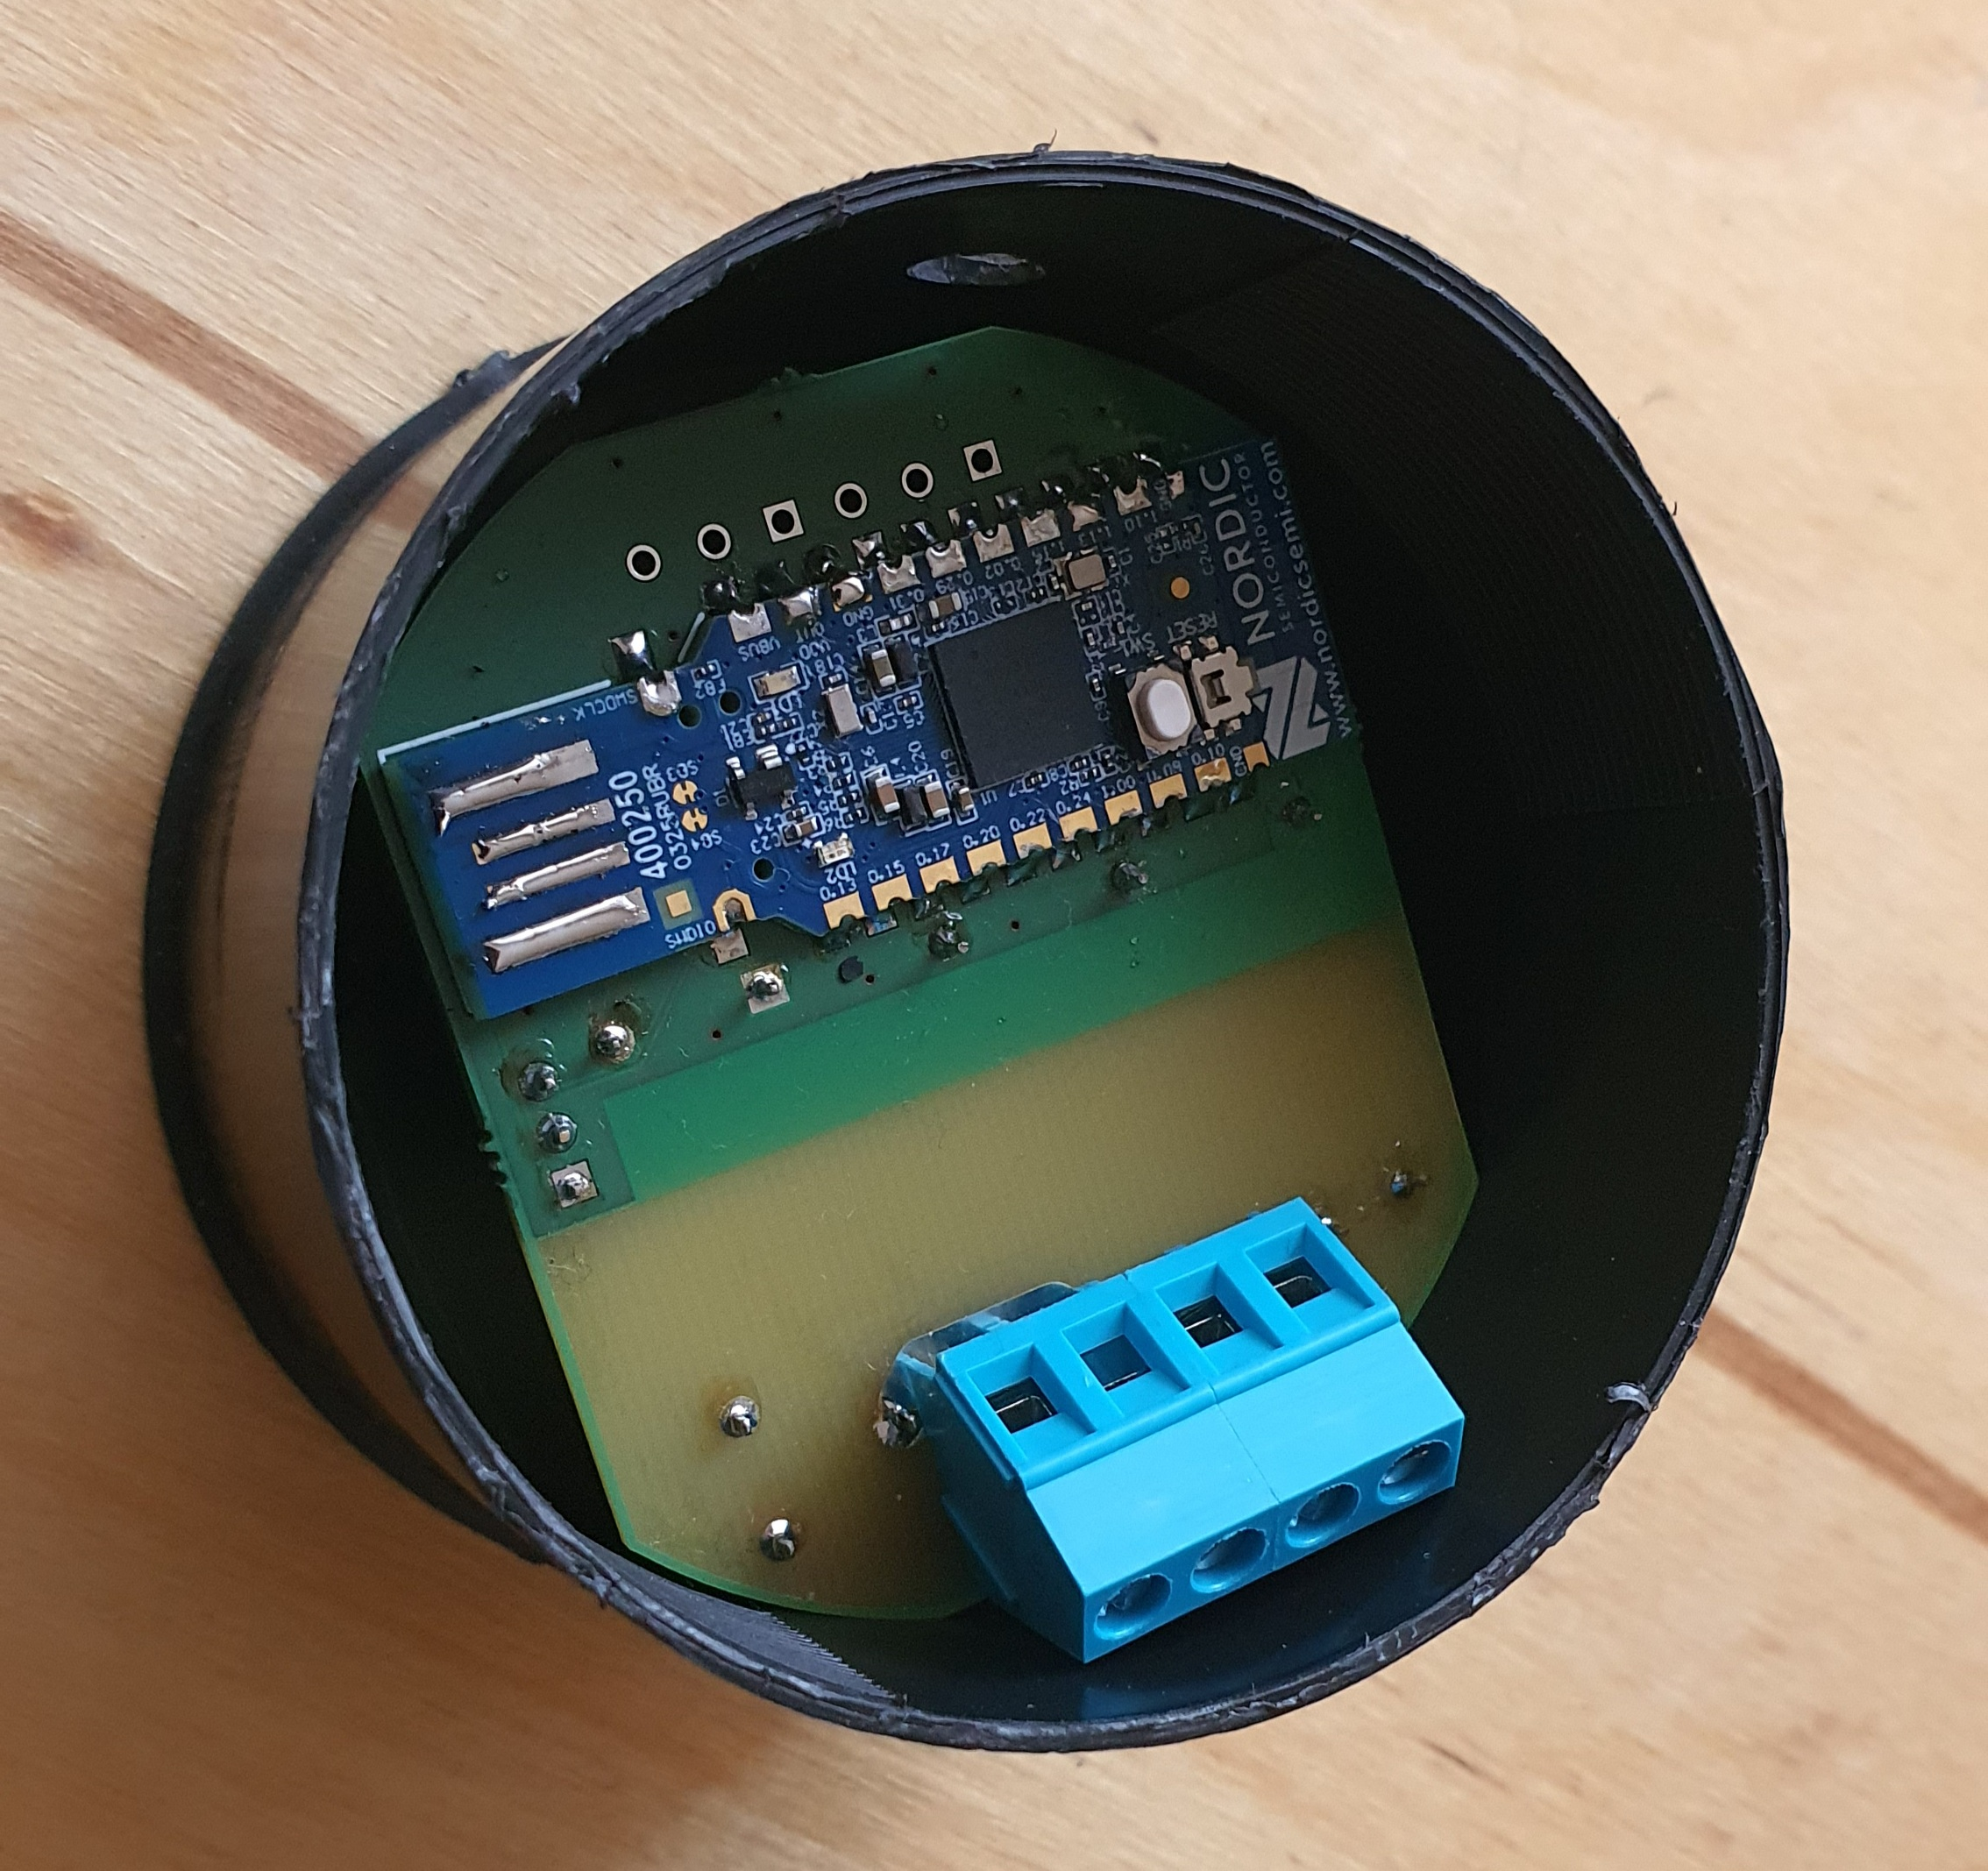
\includegraphics[scale=0.1]{img/realblindaccesspoint.jpg}
    \caption{Assembled Blind Access Point in the assembly box}
    \label{fig:realblindaccesspoint}
\end{figure}

\subsection{The completed Minimal Sensor Node}
\begin{figure}[!htb]
    \centering
    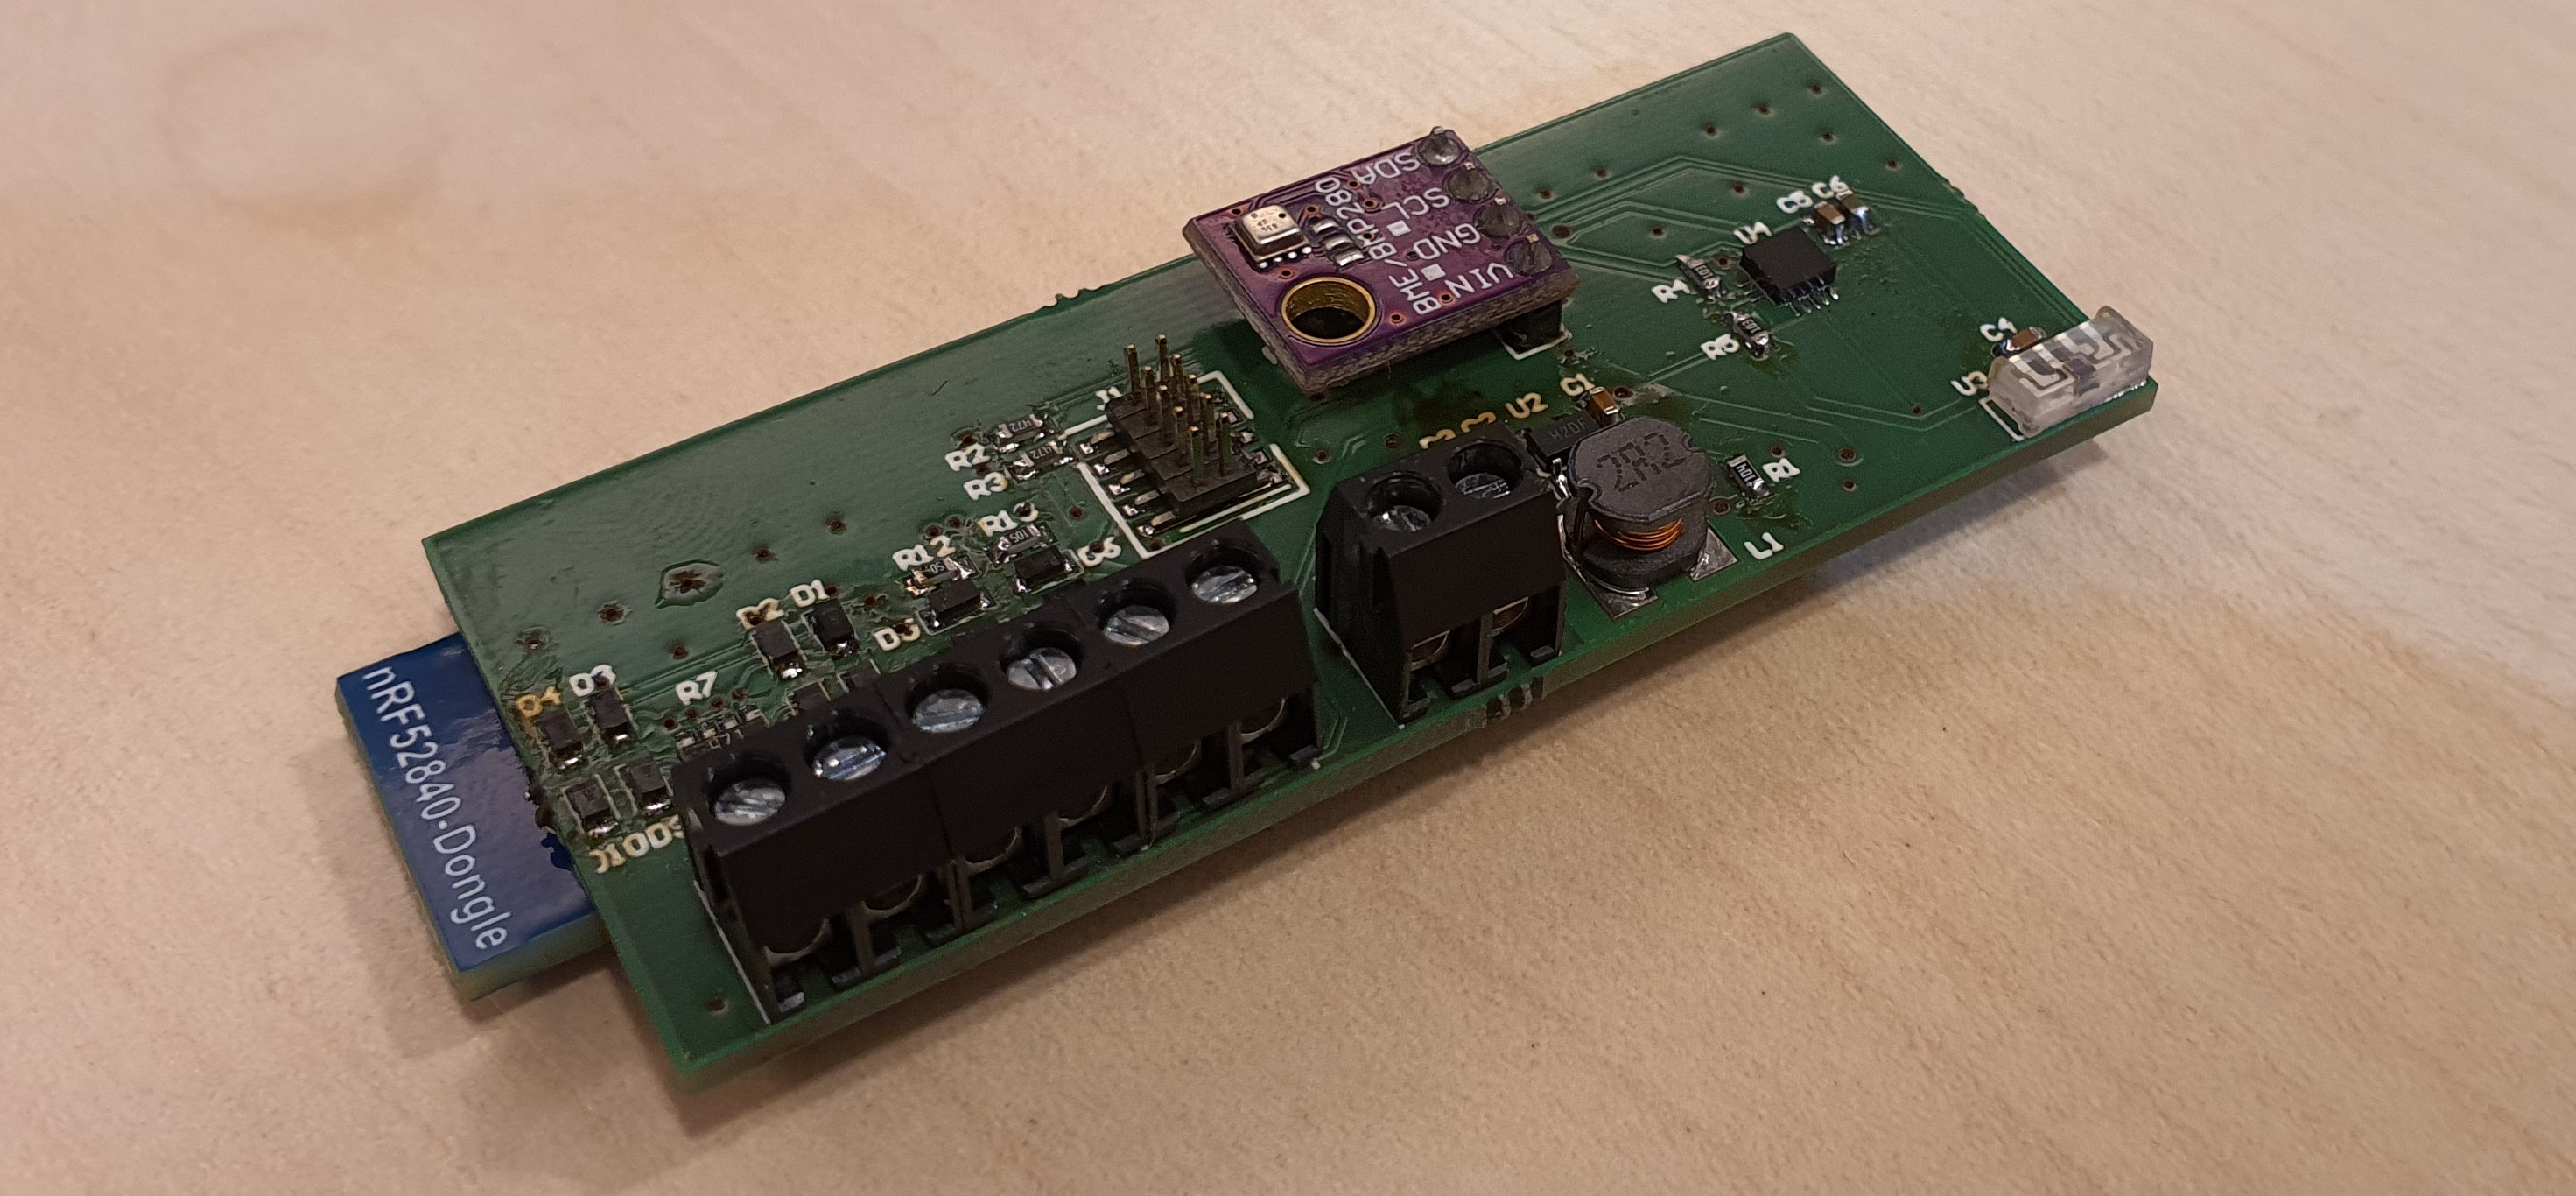
\includegraphics[width=\textwidth]{img/minimalupperside.jpg}
    \caption{Completed Minimal Sensor Node upper side}
    \label{fig:realminimalup}
\end{figure}
\begin{figure}[!htb]
    \centering
    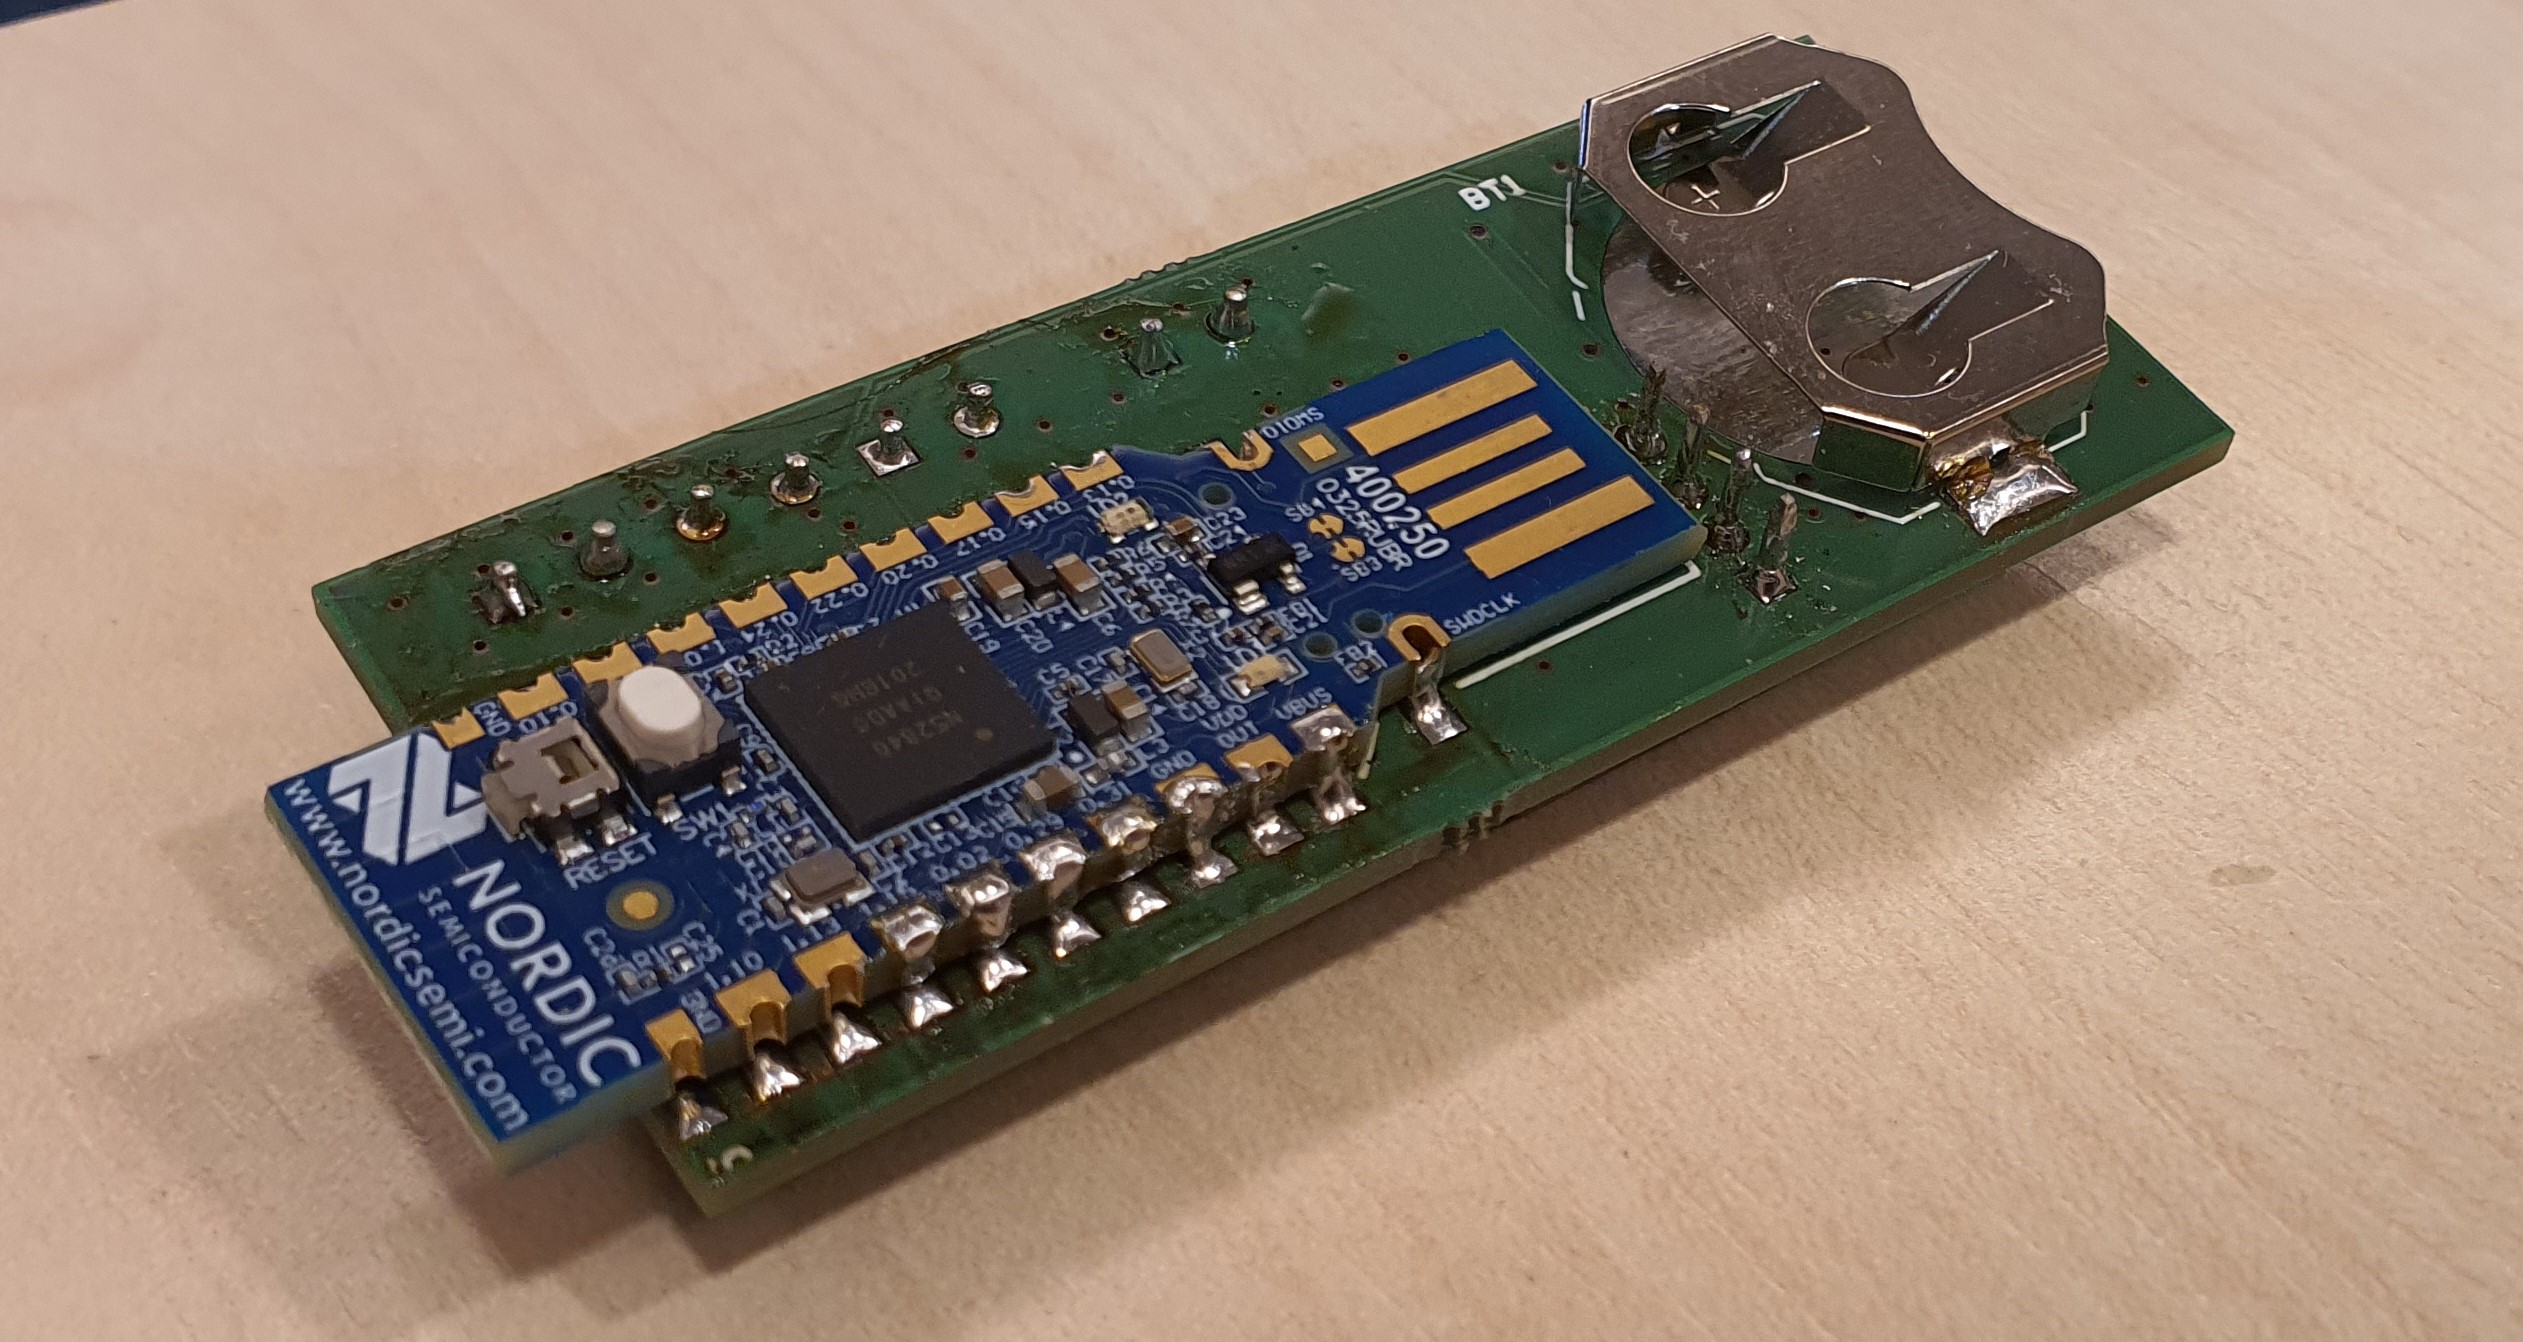
\includegraphics[width=\textwidth]{img/minimaldownside.jpg}
    \caption{Completed Minimal Sensor Node lower side}
    \label{fig:realminimaldown}
\end{figure}


\subsection{Insight}
The use cases I have presented, represent only a small part of the feasible devices. Large US companies like Apple and Google have also released several devices that support the Thread protocol. Such devices include the Apple HomePod mini and the Google Nest Hub Max. For those interested, a detailed list of Thread-certified devices is available at \href{https://www.threadgroup.org/What-is-Thread/Thread-Benefits}{Thread Group}\cite{devices}. 
\clearpage
\section{Summary}
In this bachelor's thesis, I presented the potential of Thread networks for application in smart homes as part of my research. I have described and presented in detail the Thread protocol implemented by Google, OpenThread and the roles of the tools involved. I also introduced a server-client protocol that can be implemented in embedded environments, in devices with fewer resources, with little overhead. I also introduced the Zephyr Project's revolutionary solution for processors of different architectures, which makes it easy, fast and platform-independent to implement our ideas in software form in practice and to create programs for different hardware with the same capabilities without modifying the code. It currently supports more than 350 development boards and includes different layers and protocols to easily build IoT devices. And as part of my own work, I've created a concept to make the capabilities of Thread available to consumers. This concept includes a database model and an easy-to-use GUI that anyone can use to manage their own network from anywhere. The concept also includes a ready-to-use, out-of-the-box gateway that allows users to create their own network and connect it to their home network and the Internet. I designed a device that can be hidden invisibly in the wall at the point of use, providing the backbone of the network and controlling the lighting in a room. I built 3 devices and used three of these devices in an apartment to create my own Thread network, proving the concept works. I also designed a very small device to collect environmental data of my room, which only requires a single coin-cell battery and is able to operate for years on it. 
\clearpage
\tableofcontents
\clearpage
\listoffigures
\clearpage

% \printbibliography[title={Irodalomjegyzék és hivatkozások}]
\printbibliography

\clearpage
\end{document}
